\section{Improving the pairing efficiency with SPANet} \label{section: improving}

In Section \ref{section: HH4b} the $D_{HH}$-method used for jet pairing in the Run2 $HH \to 4b$ analysis is presented. For the Run 3 analysis, in order to outperform this method, the use of the SPANet network, introduced in Section \ref{section: spanet architecture} is proposed. In this section, the different training configurations that were tested to optimize the pairing efficiency are described.


%(4 sub sections: Number of jets for the pairing, architecture, input features and results)

\subsection{Choice of the optimal inputs for the training} \label{subsection: choice of inputs}

As mentioned in Section \ref{section: spanet architecture} we can give SPANet global and sequential inputs for the training. The sequential inputs are the the ones that can have an arbitrary number of vectors per event, hence they will correspond to the information of the jets used for the pairing. The global inputs are the ones that will have a single vector per event, therefore they correspond to event-level variables.

\subsubsection{Jet multiplicity for the SPANet training}

In order to find the training that maximizes the pairing efficiency, we started by testing different configurations. As mentioned in Section \ref{subsection: topology}, the $HH \to 4b$ signature consists of four jets in the final state. Nevertheless, even if there is a signal event, more than four jets can be reconstructed in the detector due for instance to QCD multi-jet processes.
Hence, the gain in signal efficiency is checked when considering additional jets in the final state with a lower b-tag score for the pairing (reported in Table \ref{table:signal_efficiency}). The first column reports the percentage of signal where the $k^{th}$ jet is matched, i.e. the $k^{th}$ jet is matched to one of the generator-level jets. The second column reports the percentage of signal of fully matched events, i.e. the events for which four jets are matched to the four generator-level jets. Out of the total number of events, 92.9\% are fully matched and the percentage of fully matched events when considering the first 4 leading jets is 90.2\%. According to Table \ref{table:signal_efficiency}, we can observe that most of the remaining signal efficiency is gained by considering a fifth jet for the paring (2.5\% gain out of 2.7\%). 

We conclude that the highest signal efficiency is obtained by considering either 4 or 5 jets for the pairing. Therefore, SPANet will be trained using 4 and 5 jets as sequential inputs. Further tests considering 6 jets as sequential inputs have been performed, nevertheless, such a test did not increase the SPANet pairing performance, hence the choice of stopping at 5 jets for the pairing.


\begin{table}[h!]
\centering
\begin{tabular}{|p{1cm}||p{6cm}||p{6cm}|}
 \hline
 k& Signal efficiency when the $k^{th}$ jet is matched& Signal efficiency for fully matched events when the $k^{th}$ jet is matched\\
 \hline
 4 &  94.4 & 90.2\\
 5 & 2.76 & 2.52 \\
 6 & 0.27 & 0.25 \\
 $\geq$7 &  $\approx$0.03 &  $\approx$0.02 \\
 \hline
\end{tabular}
\caption{Signal efficiency when the $k^{th}$ jet is matched to a generator-level quark when considering fully and partially matched events (first column) or for only fully matched events (second column). }
\label{table:signal_efficiency}
\end{table}

To test the number of jets that will be used in the training, the performance using either 4 or 5 jets as sequential inputs is compared. As a first figure of merit for the SPANet pairing performance we employ the inclusive pairing efficiency and the inclusive total pairing efficiency. The pairing efficiency is defined as follows:

\begin{equation*}
    \text{Pairing efficiency}=\frac{\text{Correctly fully matched events}}{\text{Total number of fully matched events}}
\end{equation*}

However, as previously mentioned, the number of fully matched events is larger when considering a fifth jet for the pairing, hence to account for this difference, the total pairing efficiency is introduced as:
\vspace{-0.2cm}
\begin{eqnarray*}
\text{Total efficiency} & = & \text{Pairing efficiency} \times \text{Fraction of fully matched events} \\
% & = & \frac{\text{Correctly fully matched events}}{\text{Total number of fully matched events}} \times \frac{\text{Total number of fully matched events}}{\text{Total number of events}} \\
& = &\frac{\text{Correctly fully matched events}}{\text{Total number of events}}     
\end{eqnarray*}

Table \ref{table: First comparison} summarizes these results by showing the configuration of the training as well as the pairing efficiency and the total pairing efficiency. The variables used in the various configurations are defined in Section \ref{subsection: kinematic vars}.

\begin{table}[h!]
\centering
\begin{tabular}{|M{2cm}|M{5cm}|M{2cm}|M{2cm}|M{2cm}|}
 \hline
 Training  & Configuration &  Pairing efficiency & Fraction of fully matched events & Total pairing efficiency \\
 \hline
 4 jets &  
4 jets for the pairing 
 \begin{itemize}[itemsep=0.01em]
    \item \pt
    \item $\eta$
    \item $\phi$
    \item b-tag
 \end{itemize} 
 
  & 0.984 & 0.901 & 0.887 \\
 \hline
 4 jets 5 global & 
4 jets for the pairing and 5$^{th}$ global
 \begin{itemize}[itemsep=0.01em]
    \item \pt
    \item $\eta$
    \item $\phi$
    \item b-tag
 \end{itemize} 
 & 0.984 & 0.901 & 0.887\\
 \hline
  5 jets & 

5 jets for the pairing 
 \begin{itemize}[itemsep=0.01em]
    \item \pt
    \item $\eta$
    \item $\phi$
    \item b-tag
 \end{itemize} 

  &  0.942 & 0.926 &  0.872 \\
 \hline
\end{tabular}
\caption{Comparison of the training configurations to determine the number of jets considered for the pairing.  The name of the trainings as well as the configuration, i.e. the input features the network uses are defined. The performance of these trainings is compared by showing the pairing efficiency and the total pairing efficiency.}
\label{table: First comparison}
\end{table}

As previously explained, the global variables only add event-level information, therefore in the training using 4 jets 5 global, the fifth jet adds information on the kinematics of the system but is not used for the pairing.

In order to compare the trainings presented in Table \ref{table: First comparison}, the total pairing efficiency is used as a figure of merit since it takes into consideration the fraction of fully matched events.
We conclude that using the training configurations described in Table \ref{table: First comparison}; using 4 jets and 5$^{\text{th}}$ global or 4 jets as inputs results in a better pairing performance. Nevertheless, by considering a 5$^{\text{th}}$ jet as either a global input or for the pairing can help the reconstruction performance by the SPANet network since it provides additional information about the event. Therefore, in Section \ref{subsubsection: input features and results} different configurations using 4 jets with a 5$^{\text{th}}$ global and 5 jets as inputs. In the new configurations we either vary the kinematical information of the jets or some of the hyperparameters of the model. 

\newpage

\subsubsection{SPANet architecture} \label{large vs lite model}
In the following, we will be comparing two different SPANet architectures. The so-called "Large model" that employs the default SPANet hyperparameters and the so-called "Lite Model", which uses the values of some of the hyperparameters shown in \cite{ATLASparam}. Some features of these models are shown in Table \ref{table:comparison_models}. The main difference between these models is given by the trainable parameters that make the Large model, as the name suggests, significantly larger than the Lite model.

\begin{table}[h!]
    \centering
     \begin{tabular}{|c||c|c|}
      \hline
         & Large model &  Lite model\\ 
      \hline
      Hidden dimensions & 64 &  32\\ 
      \hline
      Transformer dimension& 64 & 64 \\ 
      \hline
      Embedding layers & 10 & 8 \\ 
      \hline
      Encoder layers & 6 & 6 \\ 
      \hline
      Trainable parameters & \textbf{2.2 M} & \textbf{0.5M} \\ 
      \hline
      Learning rate & 0.0015 & 0.00659 \\ 
      \hline
      Batch size & 2048 & 2048 \\ 
      \hline
      Optimizer & AdamW & AdamW \\ 
      \hline
      Number of epochs & 50 & 50 \\
      \hline
    \end{tabular}
    \caption{Comparison of the hyperparameters used in the Large and Lite models. The definition of these hyperparameters was given in Section \ref{section: spanet architecture}.}
    \label{table:comparison_models}
\end{table}


\subsubsection{Input features and results} \label{subsubsection: input features and results}

Tables \ref{table:5 jets trainings} and \ref{table:4 jets trainings} present the different training configurations that are compared. For each training configuration, different input features are given to the network. We vary either the architecture or the kinematic information of the jets. Moreover, Tables \ref{table:5 jets trainings} and \ref{table:4 jets trainings} report the results for the inclusive pairing and total pairing efficiencies. For either 5 jets or 4 jets 5 global, the best performance is obtained by using \pt regressed and the Lite model. 

\begin{table}[h!]
\centering
\begin{tabular}{|M{2.5cm}|M{5.25cm}|M{1.75cm}|M{1.75cm}|M{1.75cm}|}
 \hline
 Training  & Configuration &  Pairing efficiency  & Fraction of fully matched events & Total pairing efficiency \\
 \hline
 5 jets & \raggedright \footnotesize \begin{itemize}[itemsep=0.001em]
    \item \pt
    \item $\eta$
    \item $\phi$
    \item b-tag
    \item Large model
 \end{itemize} & 0.942 & 0.926 & 0.872 \\
 \hline
 5 jets with b-tag preselection \pt regressed & \raggedright  \footnotesize \begin{itemize}[itemsep=0.001em]
    \item \pt
    \item $\eta$
    \item $\phi$
    \item b-tag
    \item Large model
    \item Fifth jet has a b-tag above the medium working point
 \end{itemize}  & 0.975 & 0.913 & 0.890 \\
 \hline
  5 jets \pt regressed and Lite model & \raggedright \footnotesize \begin{itemize}[itemsep=0.001em]
    \item \pt regressed
    \item $\eta$
    \item $\phi$
    \item b-tag
    \item Lite model
 \end{itemize} &  0.969 & 0.926 & 0.897\\
 \hline
 5 jets \pt regressed, Lite model and b-tag preselection & \raggedright \footnotesize \begin{itemize}[itemsep=0.001em]
    \item \pt
    \item $\eta$
    \item $\phi$
    \item b-tag
    \item Lite model
    \item Fifth jet has a b-tag above the medium working point
 \end{itemize} 
  & 0.977 & 0.913 & 0.892\\
 \hline
\end{tabular}
\caption{Different trainings configurations with 5 jets as sequential inputs.}
\label{table:5 jets trainings}
\end{table}

\begin{table}[h!]
\centering
\begin{tabular}{|M{2.5cm}|M{5.25cm}|M{1.75cm}|M{1.75cm}|M{1.75cm}|}
 \hline
 Training  & Configuration &  Pairing efficiency  & Fraction of fully matched events & Total pairing efficiency \\
 \hline
 4 jets 5 global & \raggedright \footnotesize \begin{itemize}[itemsep=0.001em]
    \item \pt
    \item $\eta$
    \item $\phi$
    \item b-tag
    \item Large model
 \end{itemize} & 0.984 & 0.901 & 0.887 \\
 \hline
 4 jets 5 global \pt regressed & \raggedright  \footnotesize \begin{itemize}[itemsep=0.001em]
    \item \pt regressed
    \item $\eta$
    \item $\phi$
    \item b-tag
    \item Large model
 \end{itemize}  & 0.985 & 0.901 & 0.887 \\
 \hline
  4 jets 5 global \pt regressed and Lite model & \raggedright \footnotesize \begin{itemize}[itemsep=0.001em]
    \item \pt regressed
    \item $\eta$
    \item $\phi$
    \item b-tag
    \item Lite model
 \end{itemize} &  0.986 & 0.901 & 0.888\\
 \hline
 4 jets 5 global Lite model & \raggedright \footnotesize \begin{itemize}[itemsep=0.001em]
    \item \pt
    \item $\eta$
    \item $\phi$
    \item b-tag
    \item Lite model
 \end{itemize}  & 0.983 & 0.901 & 0.886 \\
 \hline
 4 jets 5 global with b-tag preselection & \raggedright \footnotesize \begin{itemize}[itemsep=0.001em]
    \item \pt
    \item $\eta$
    \item $\phi$
    \item b-tag
    \item Large model
    \item Fifth jet given as global input has a b-tag above the medium working point
 \end{itemize} 
  & 0.984 & 0.901 & 0.886\\
 \hline
\end{tabular}
\caption{Different training configurations with 4 jets as sequential inputs.}
\label{table:4 jets trainings}
\end{table}

It is also possible to compare the total pairing efficiency as a function of $m_{HH}$, as shown in Figures \ref{fig: comp 4j5g} and \ref{fig: comp 5j}. Figure \ref{fig: comp 4j5g} shows the comparison of the different trainings presented in Table \ref{table:4 jets trainings}. We observe that varying the configurations with 4 jets and 5$^{th}$ global as inputs does not have a significant impact on the total pairing efficiency. Figure \ref{fig: comp 5j} presents the results of the trainings described in Table \ref{table:5 jets trainings}. Contrary to what was said for 4 jets and 5$^{th}$ global, we observe an important difference in the pairing efficiency when varying the configuration.

\begin{figure} [h!]
    \centering
    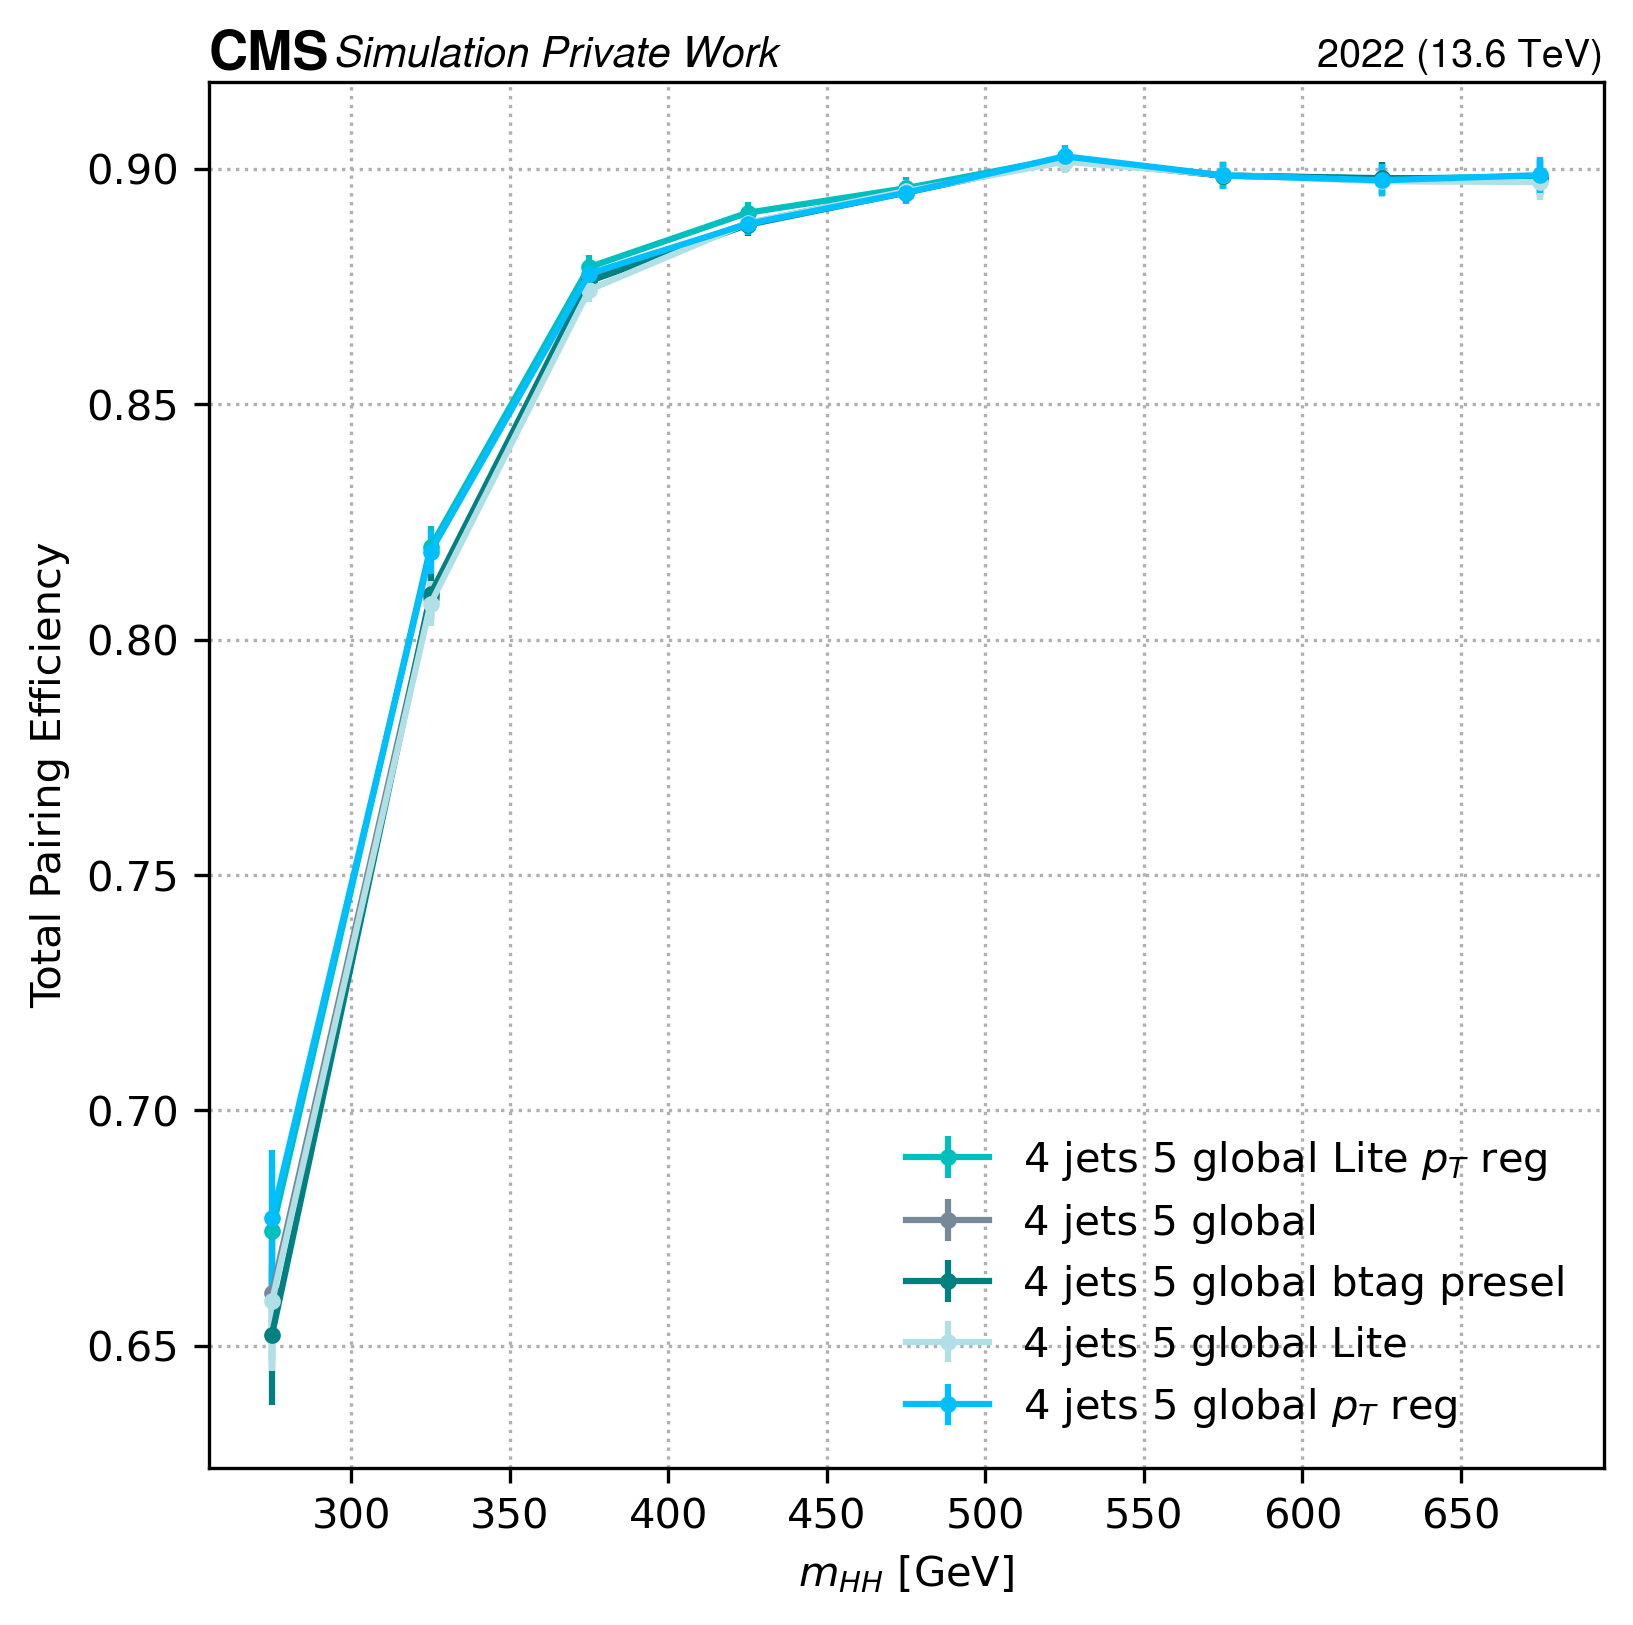
\includegraphics[width=0.6\linewidth]{Images/6.Improving/Imput Comparisons/4j5g training comp.png}
    \caption{Comparison of the total pairing efficiency as a function of $m_{HH}$ for the different trainings presented in Table \ref{table:4 jets trainings} using 4 jets and a 5$^\text{th}$ global as input.}
    \label{fig: comp 4j5g}
\end{figure}

\begin{figure}[h!]
    \centering
    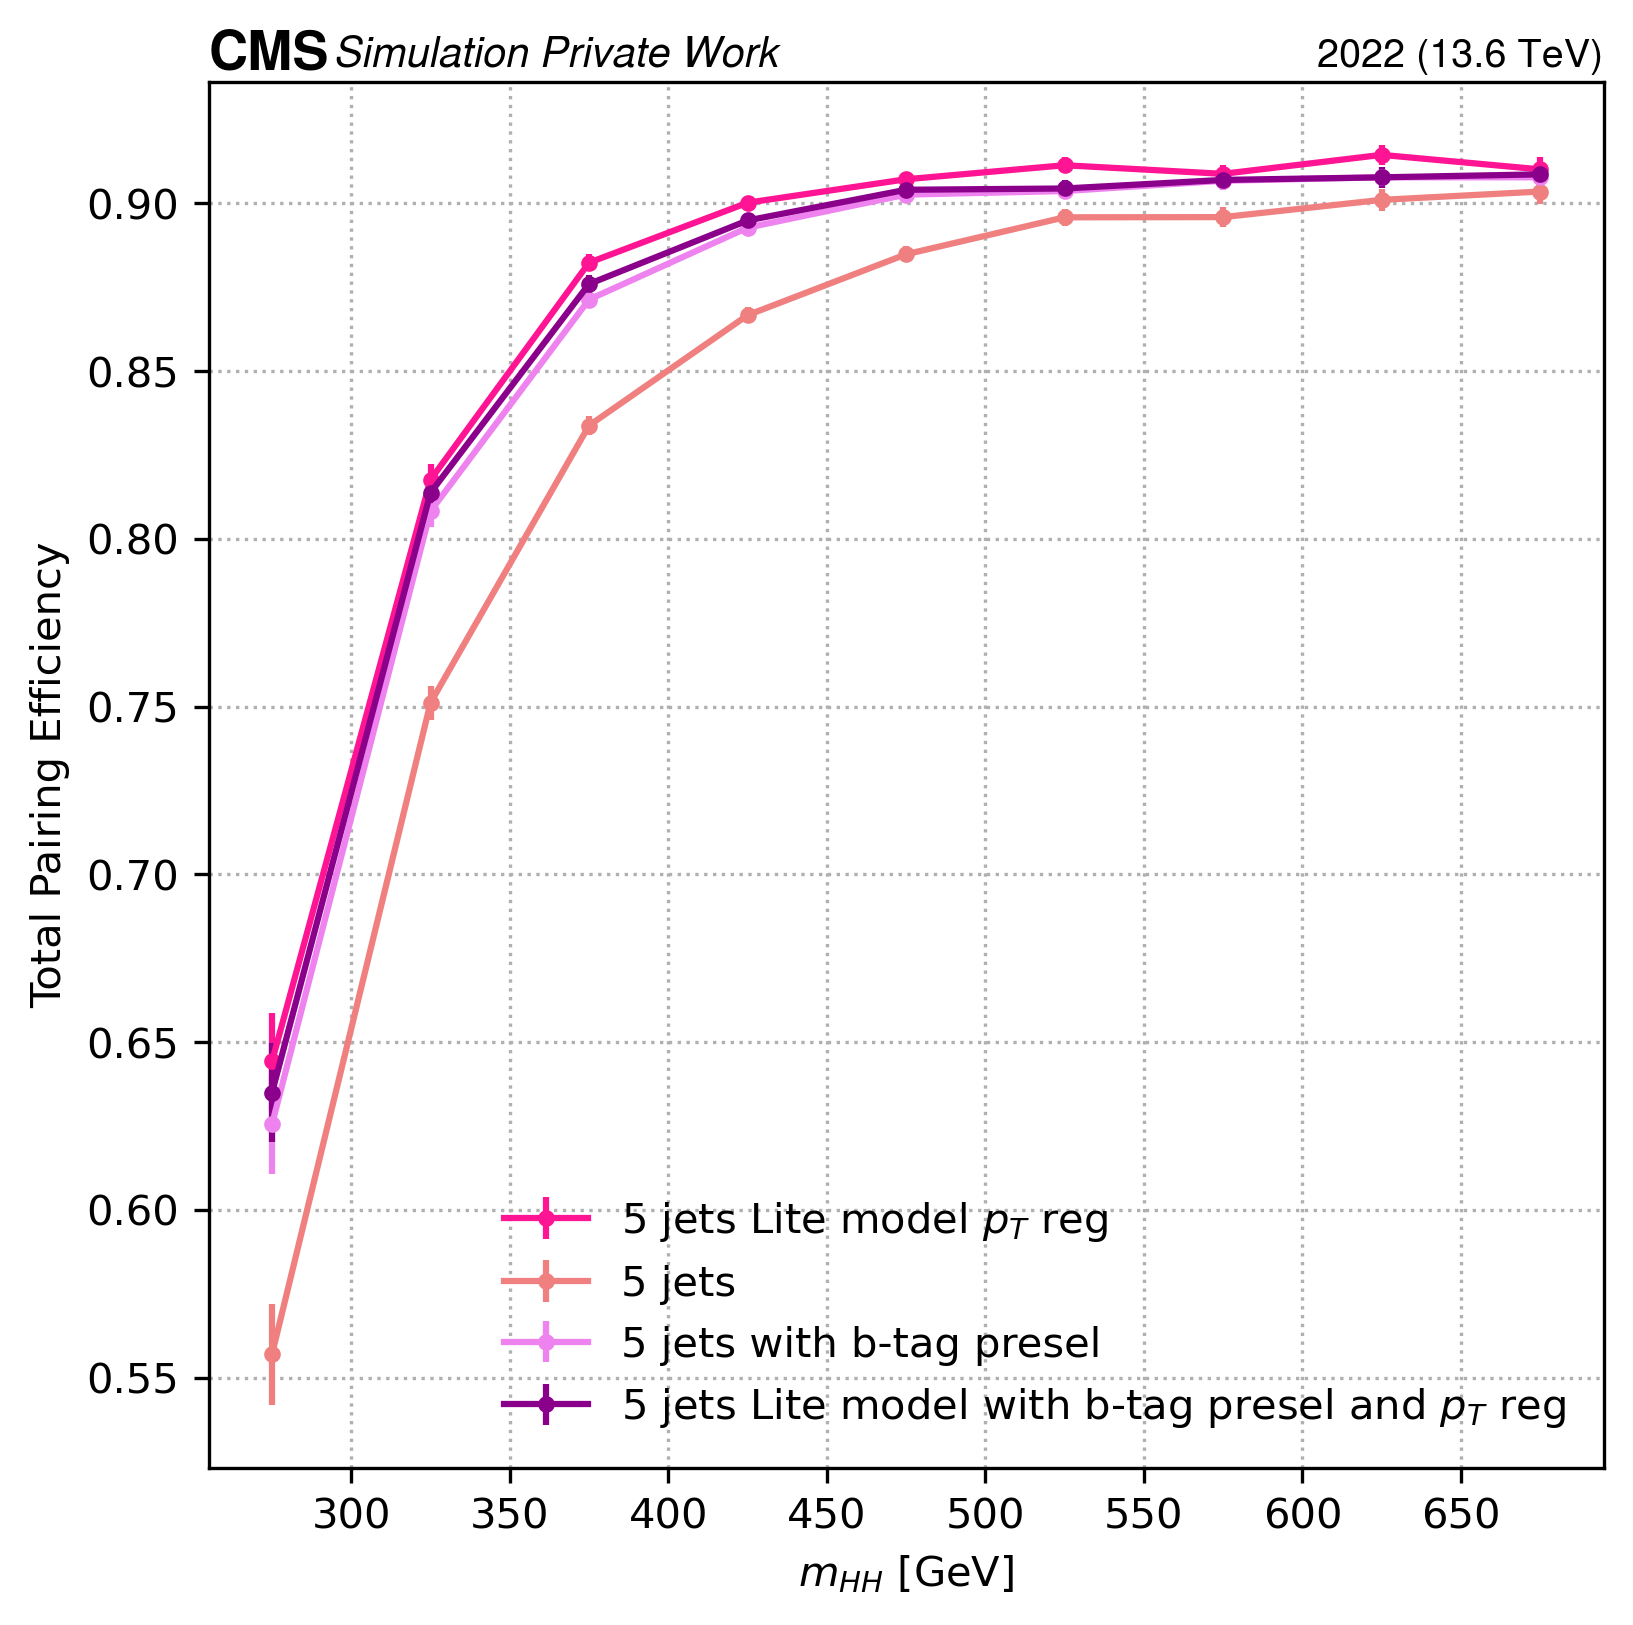
\includegraphics[width=0.6\linewidth]{Images/6.Improving/Imput Comparisons/5j training comp.png}
    \caption{Comparison of the total pairing efficiency as a function of $m_{HH}$ for the different trainings presented in Table \ref{table:5 jets trainings} using 5 jets as inputs.}
    \label{fig: comp 5j}
\end{figure}



The next step is to compare these two models to the performance of the previous $D_{HH}$-method presented in Section \ref{section: HH4b}. The comparison is performed for events for which we have $\Delta D_{HH} > 30$ GeV, as we only implemented this method for these events. In Figure \ref{fig: 2 best models comp} we show that the two SPANet models outperform the $D_{HH}$-method. 

\begin{figure}[h!]
    \centering
    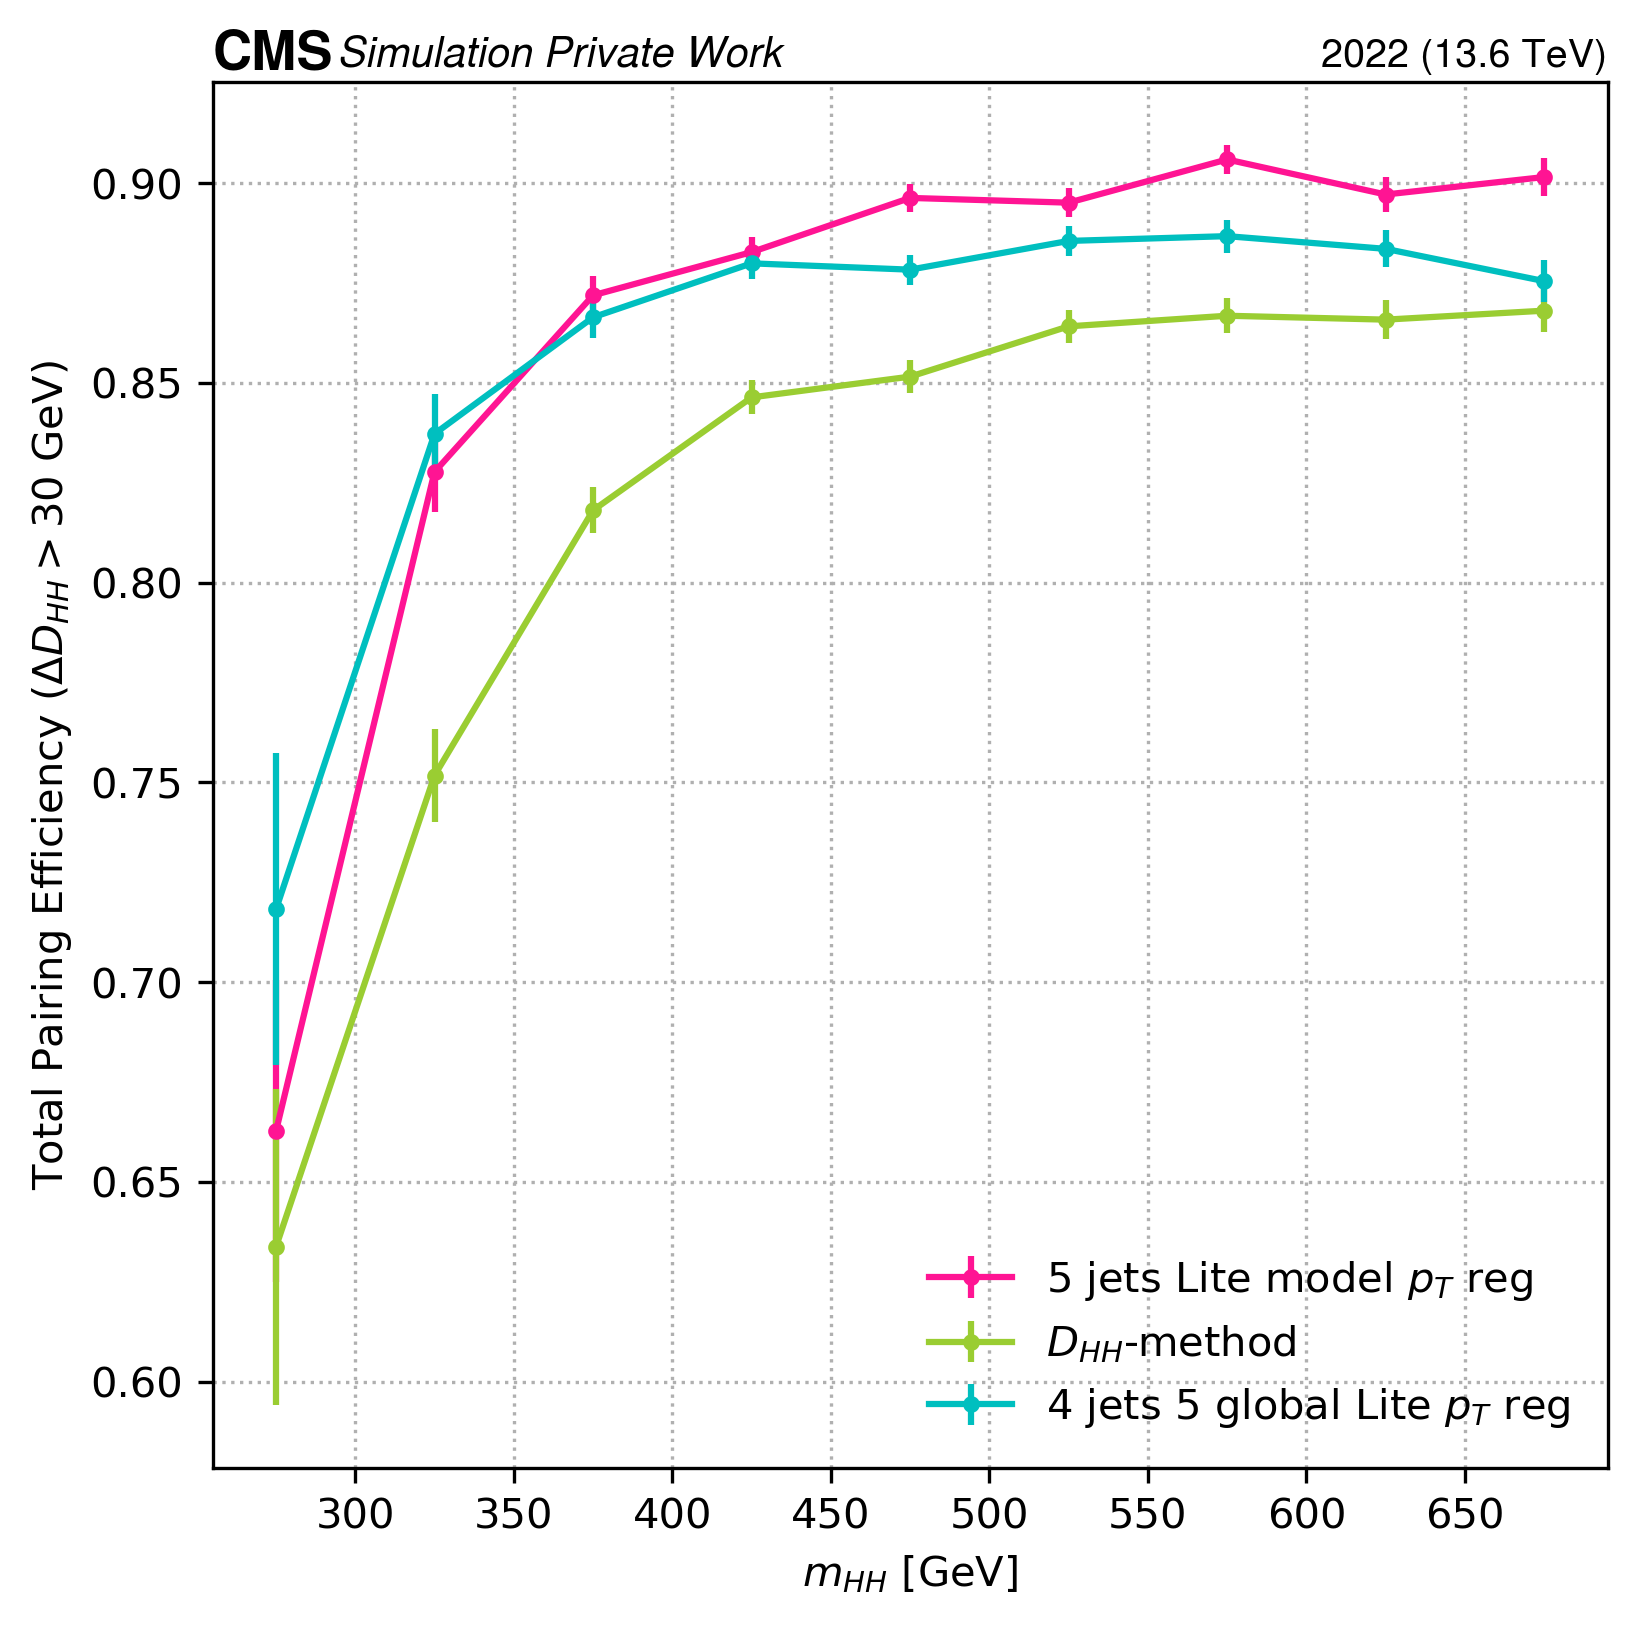
\includegraphics[width=0.6\linewidth]{Images/6.Improving/Imput Comparisons/2 best models comp run2 .png}
    \caption{Comparison of the total pairing efficiency for events where $\Delta D_{HH} > 30$. The performance of the 5 jets Lite model (with \pt regressed) defined in Table \ref{table:5 jets trainings} and 4 jets 5 global Lite model (with \pt regressed) defined in  Table \ref{table:4 jets trainings} are compared. These are the two best performing models obtained using SPANet and their performance is also compared to the performance of the $D_{HH}$-method described in Section \ref{section: HH4b} that was used for the pairing in Run 2. }
    \label{fig: 2 best models comp}
\end{figure}


\clearpage

\noindent In conclusion, we converged on two optimized pairing models:

\begin{itemize} [itemsep=0.1em]
    \item 4 jets as sequential inputs with a 5th global jet using the \pt regressed $\eta, \phi$ and btag of the jets employing the Lite model
    \item 5 jets as sequential inputs using the \pt regressed $\eta, \phi$ and btag of the jets employing the Lite model
\end{itemize}

\noindent which have the highest total efficiency and outperform the pairing efficiency used in the $D_{HH}$-method.

The performance of these two trainings evaluated on datasets with only 4 jets in the final state is also assessed. However,  it is not a completely fair comparison because of the difference in phase space, i.e. the jet multiplicity and all observables correlated to it, between the train and the test files.  

Lastly, one training without the b-tag of the jet is performed because this observable is already used in the HH $\to$ 4b analysis in the DNN for the 2b to 4b morphing for the QCD background estimation (described in Section \ref{section: HH4b}). Therefore, there could be correlations since this variable is used for both networks. The performance without b-tagging inputs was observed to be worse than by including it in the inputs. Comparing the validation accuracy (defined in section \ref{section: spanet architecture}) shows that the 5 jets Lite model \pt regressed model without b-tag (0.875) performs significantly worse than the same model using b-tag as input (0.968). We conclude that for the following section, b-tag will be used as input variable in the trainings where we use SPANet for the pairing.


\subsection{Background mass sculpting} \label{subsection: bckg mass sculpting}
In addition to the pairing efficiency, another figure of merit used in order to select the best model is the mass sculpting of the background.  A check should be done to verify that when evaluating these models on background events a fake peak of events around the SR (defined in Section \ref{section: HH4b}) is not observed. 

In order to check the potential background mass sculpting, the models presented in the last section are evaluated on a 2b data sample (defined in Section \ref{section: HH4b}). Moreover, as explained in Section \ref{subsection:cutflows} due to the requirements of the 2b region, we have mostly background events and the signal contribution due to the mistagging of the jets is negligible. Hence, if we evaluate our model on the 2b data sample, we should not observe a peak of events in the $m_{HH}$ plane around the signal region (defined in Section \ref{section: HH4b}). In Figure \ref{fig: 2D mass dist sig}, we show the 2D mass distribution of the evaluation of our model on signal events. We observe that most of the predicted events are in the signal region. On the contrary, in Figures \ref{fig: 2D mass sculpting for 4j5g} and \ref{fig: 2D mass sculpting for 5j}, we show the 2D mass distributions of the evaluation of the two best models described in Section \ref{subsection: choice of inputs} on 2b data.

%We observe that there is not a peak of events in the signal region, which shows that the SPANet pairing algorithm is not affected by the mass sculpting. 

\begin{figure}[hbt]
    \centering
    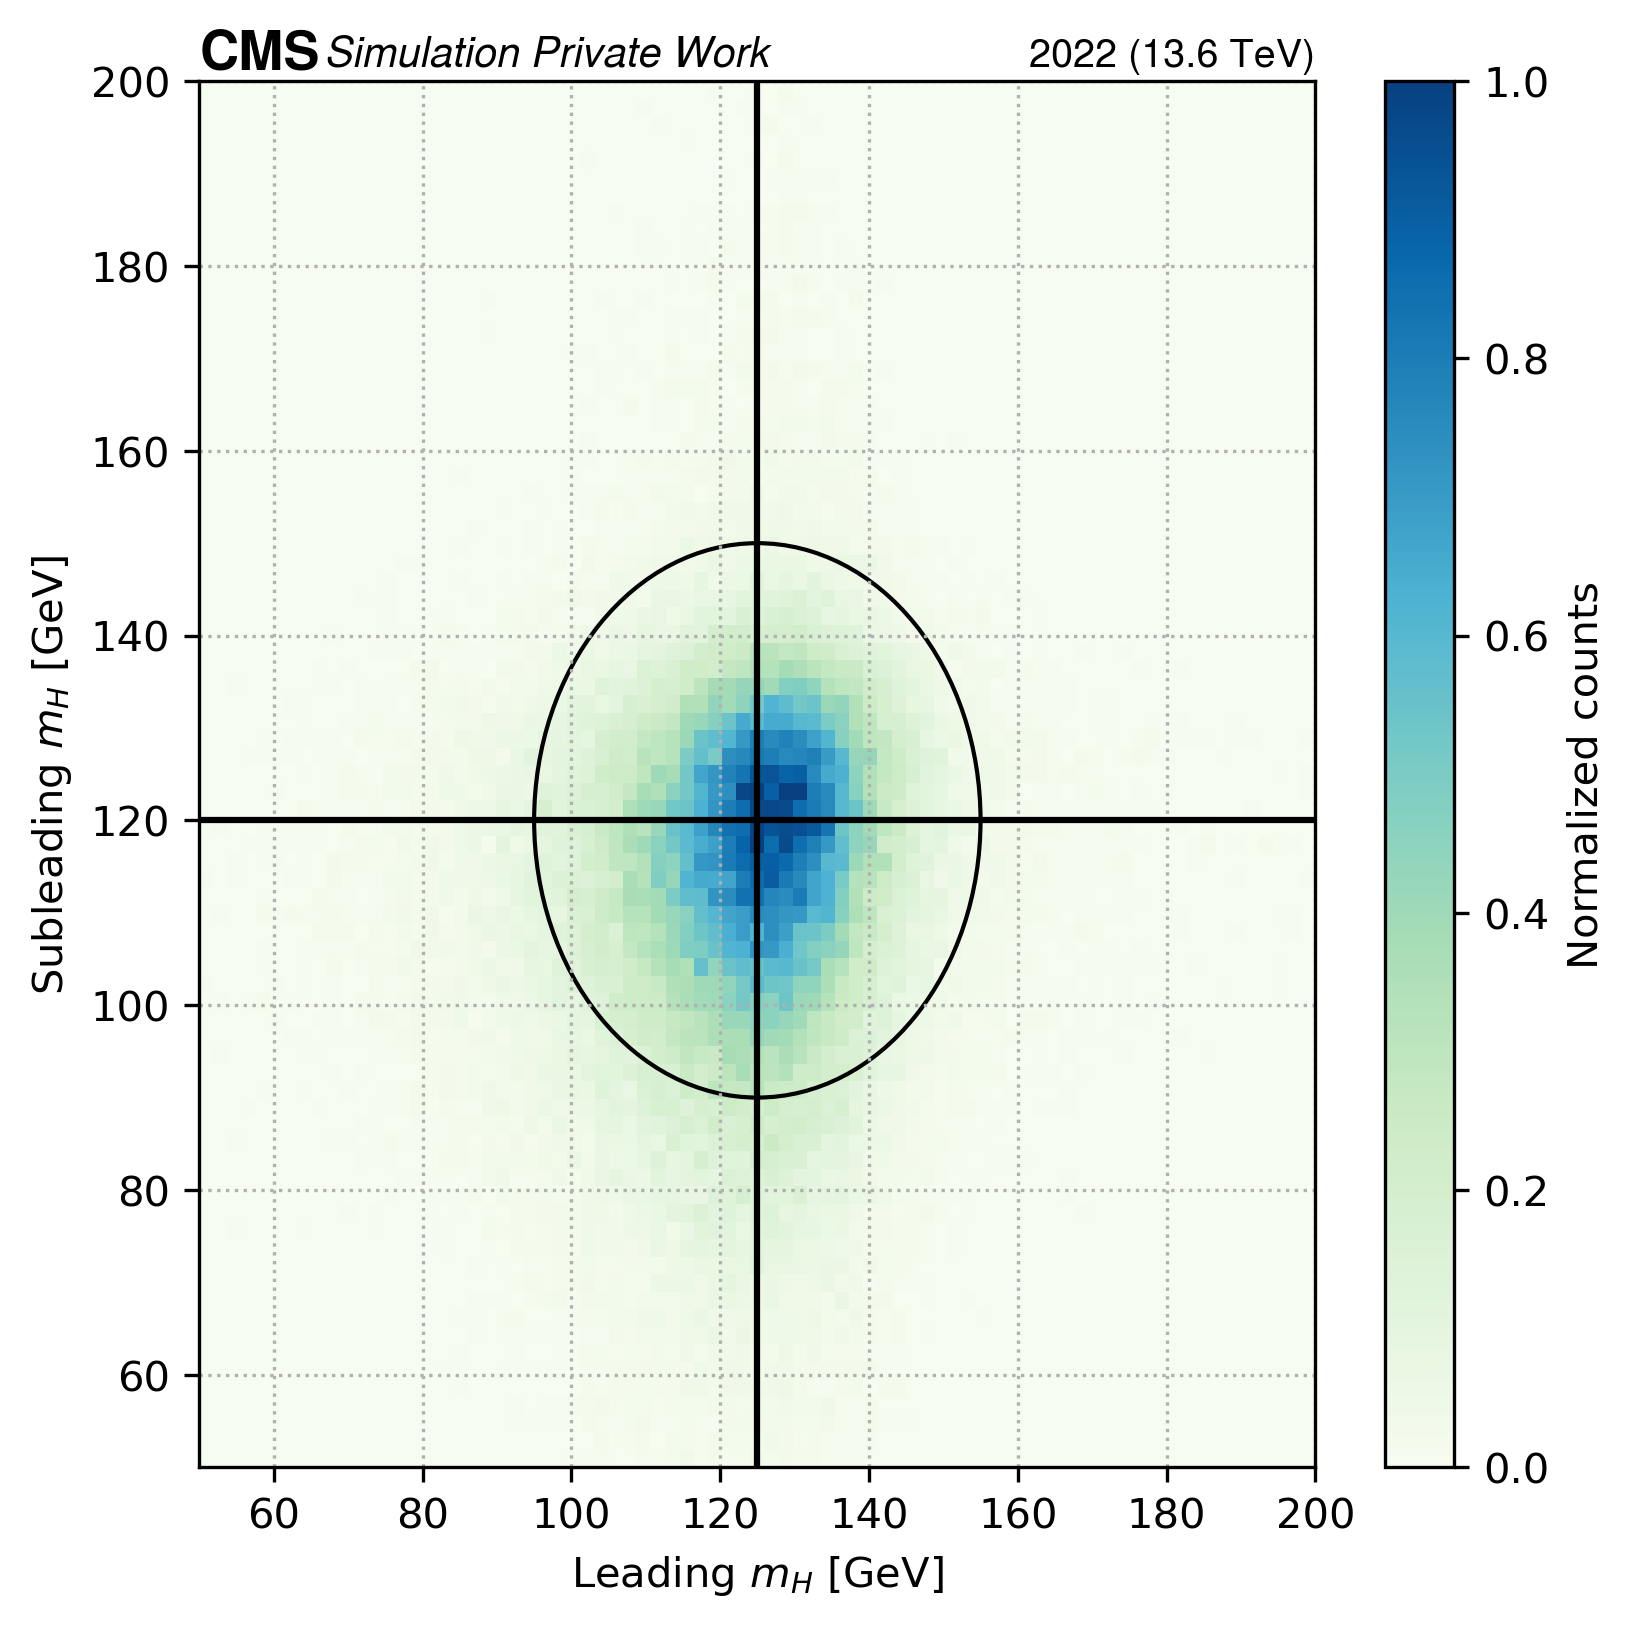
\includegraphics[width=0.6\linewidth]{Images/6.Improving/Mass sculpting/signal mhh.png}
    \caption{Higgs mass distribution of the leading Higgs and the subleading Higgs after the evaluation of the 4 jets 5$^{\text{th}}$ jet model on signal events. The vertical black line corresponds to the mass of the leading Higgs and the horizontal of the subleading Higgs. The black circle defines the SR area defined in Section \ref{section: HH4b}.}
    \label{fig: 2D mass dist sig}
\end{figure}


\begin{figure}[hbt]
    \centering
    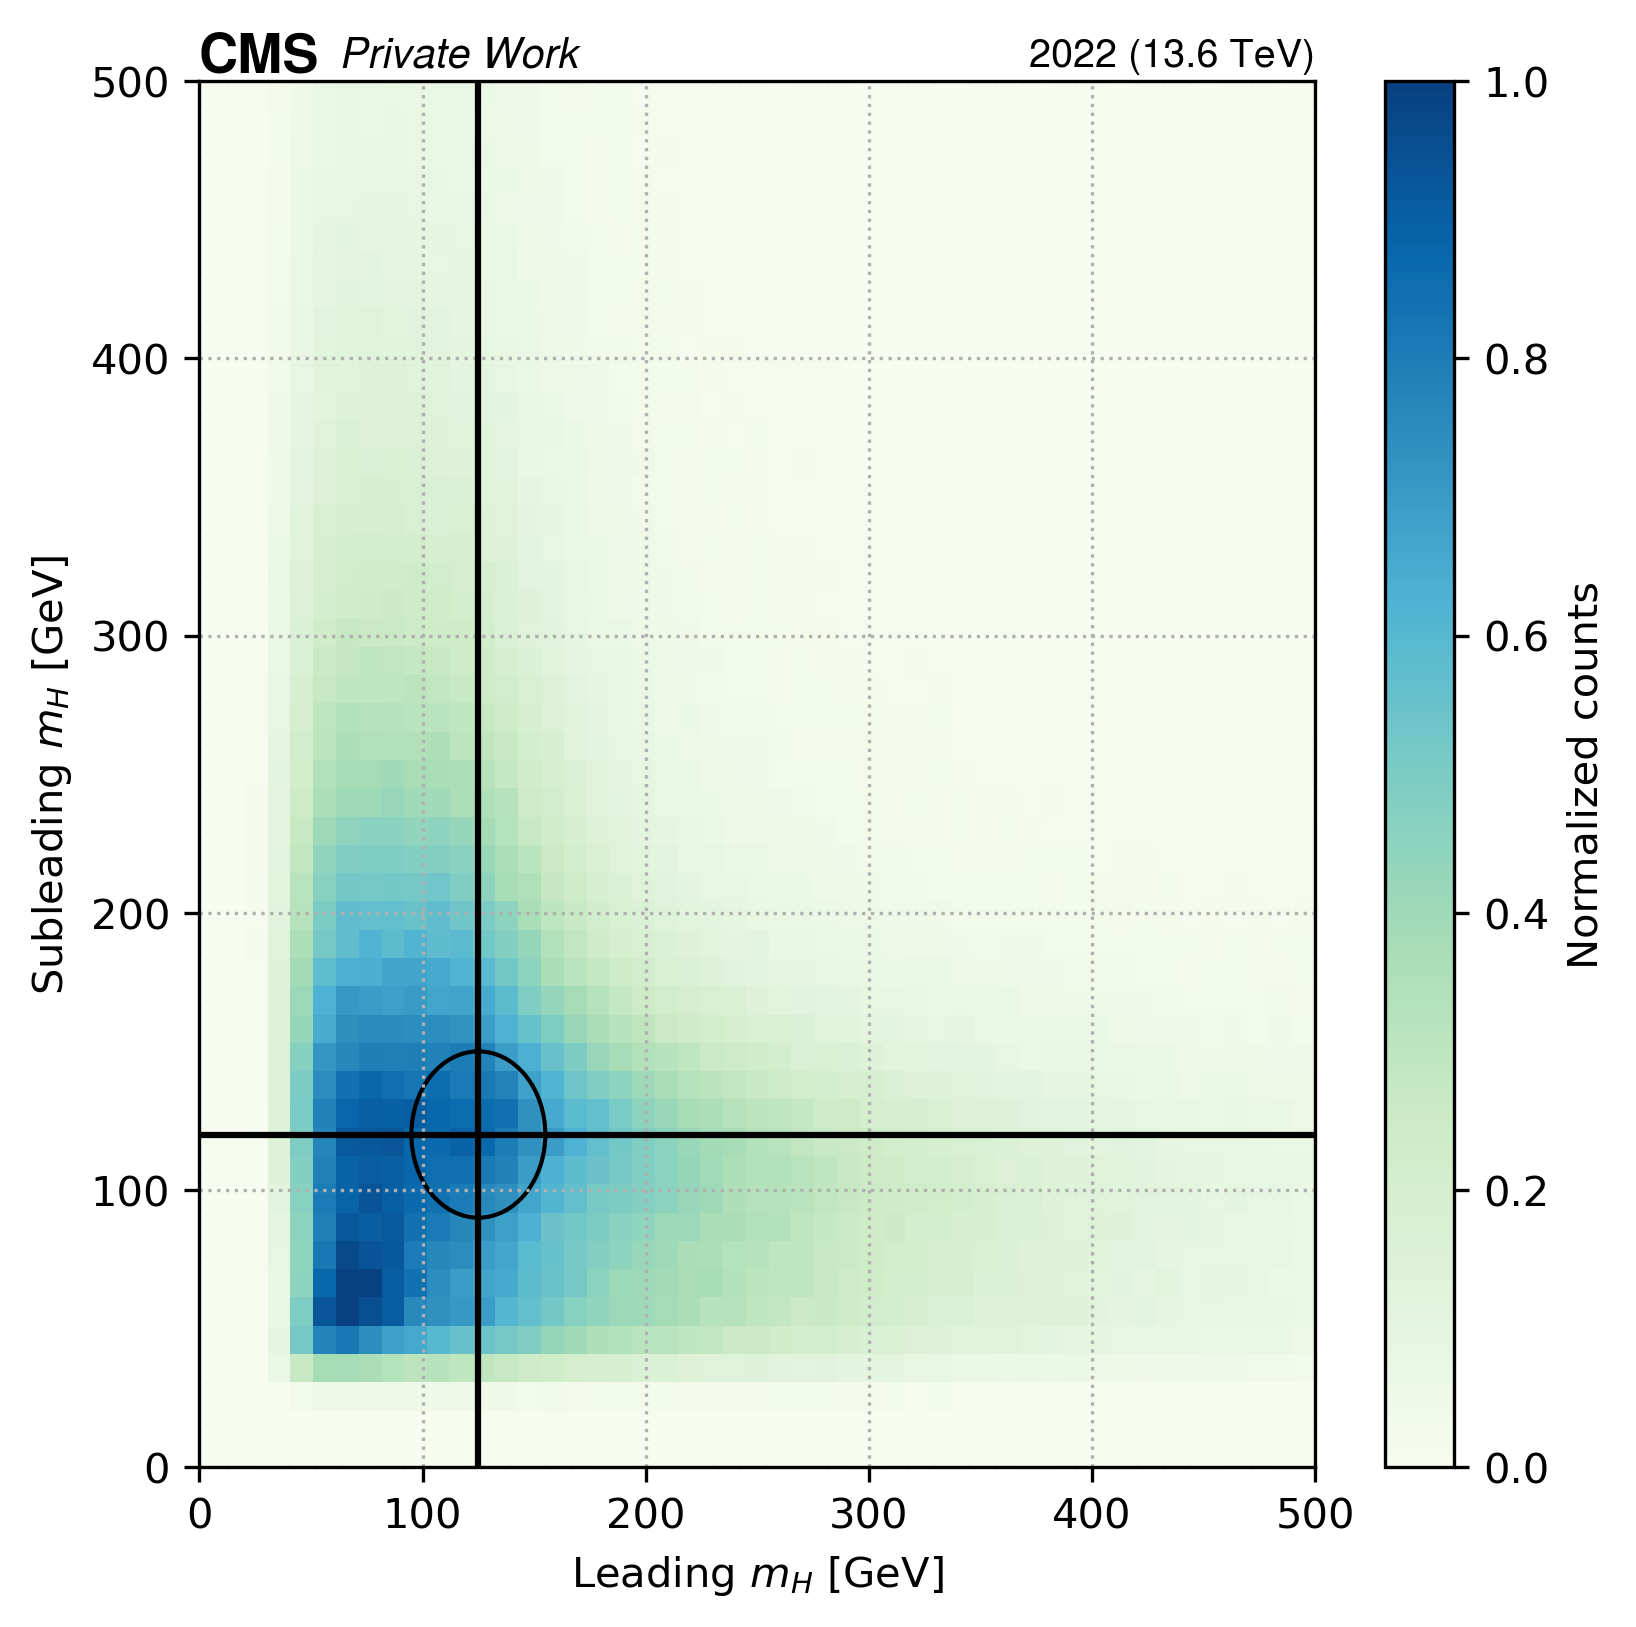
\includegraphics[width=0.6\linewidth]{Images/6.Improving/Mass sculpting/mass sculpting 4j5g.png}
    \caption{Higgs mass distribution of the leading Higgs and the subleading Higgs the evaluation of the 4 jets 5$^{\text{th}}$ jet model on 2b data. The vertical black line corresponds to the mass of the leading Higgs and the horizontal of the subleading Higgs. The black circle defines the SR area defined in Section \ref{section: HH4b}.}
    \label{fig: 2D mass sculpting for 4j5g}
\end{figure}



\begin{figure}[hbt]
    \centering
    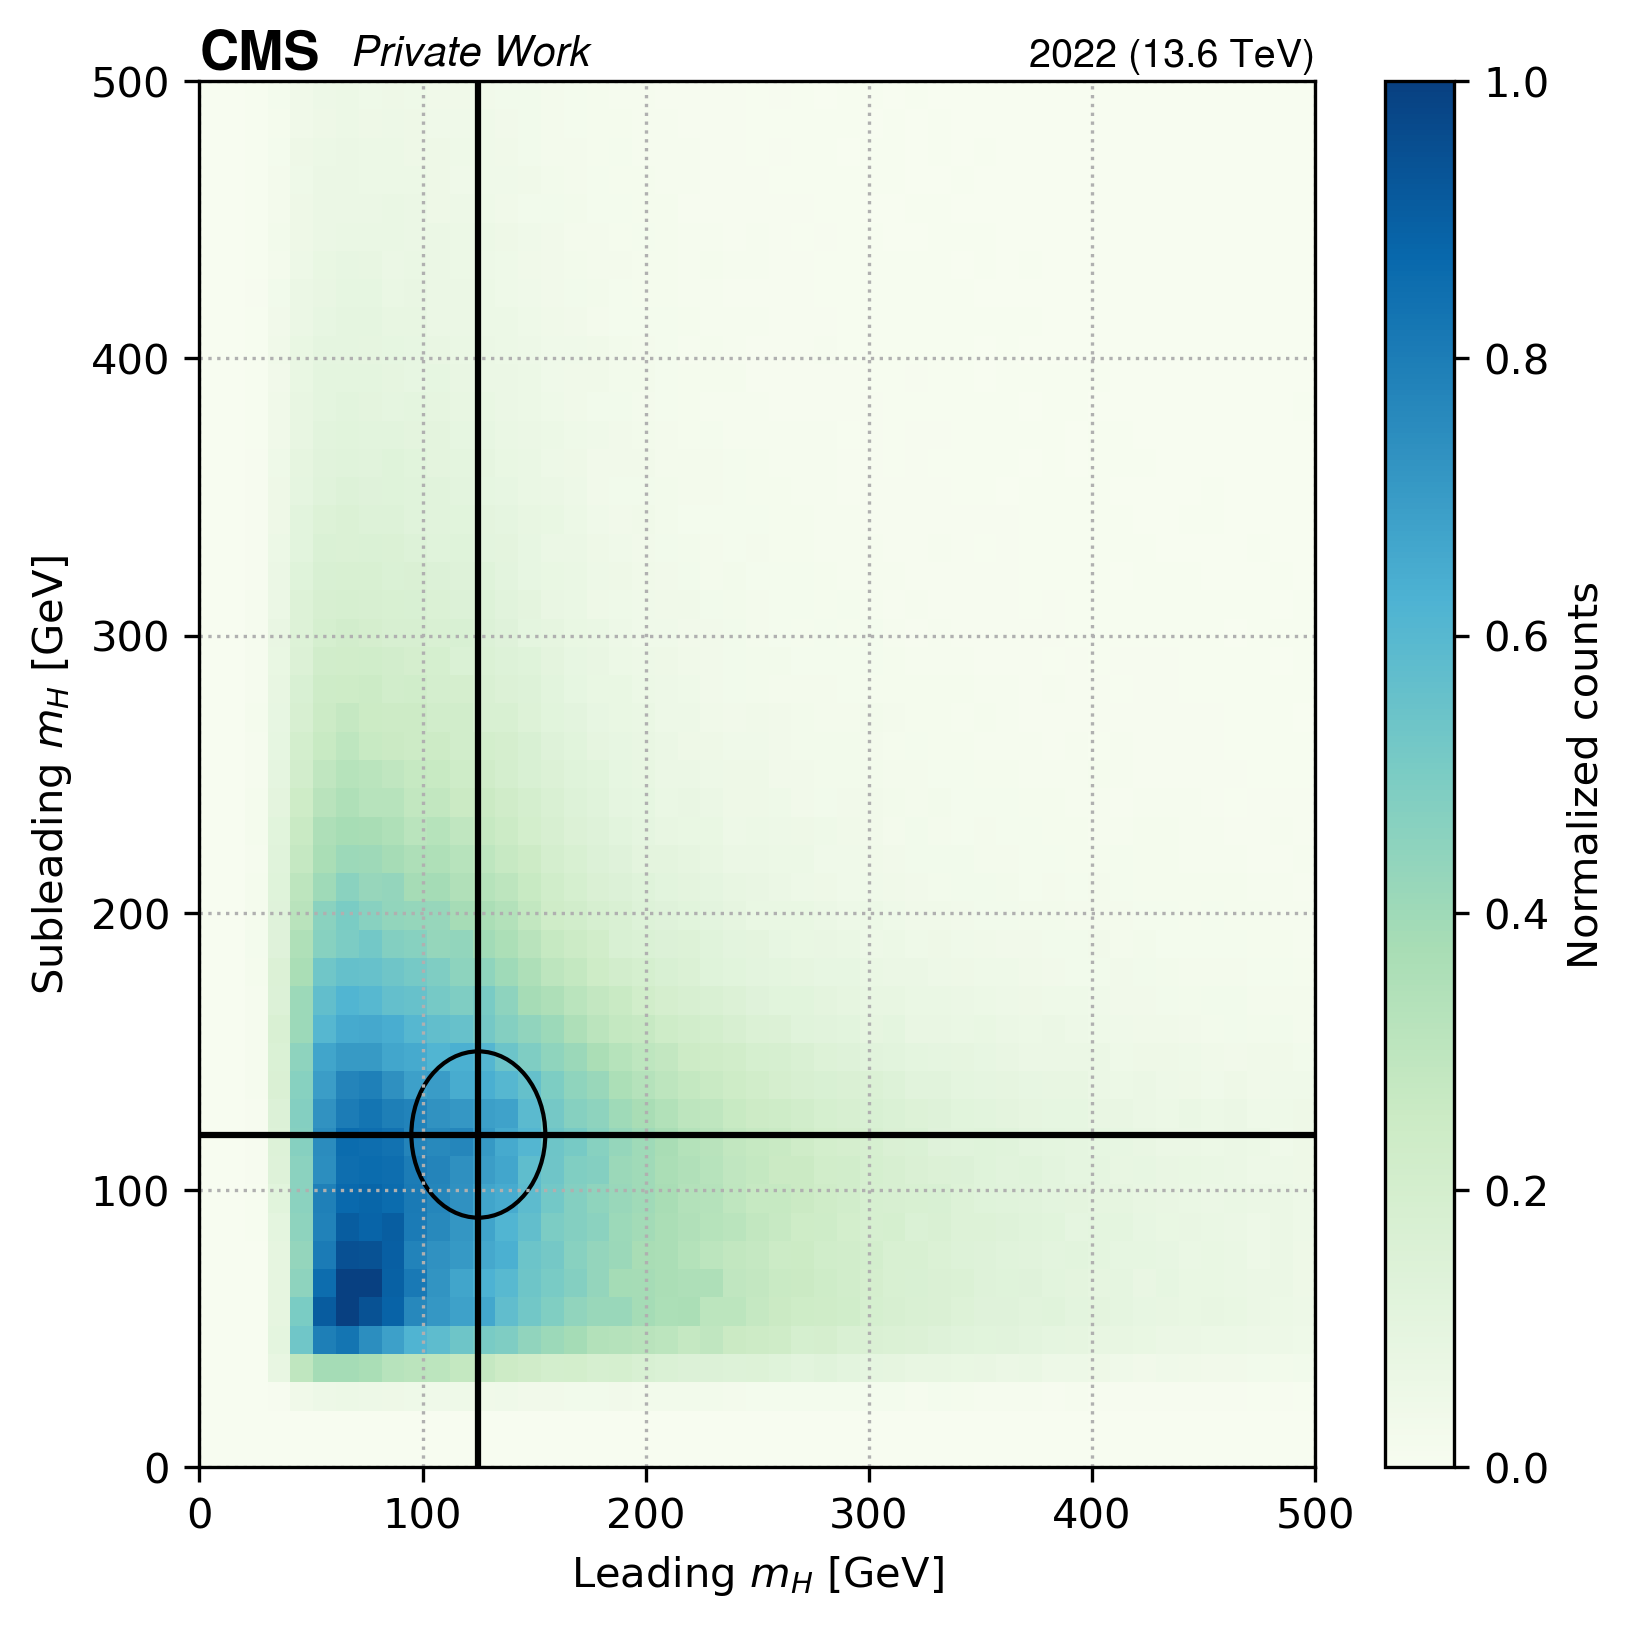
\includegraphics[width=0.6\linewidth]{Images/6.Improving/Mass sculpting/mass sculptimg 5j.png}
    \caption{Higgs mass distribution of the leading Higgs and the subleading Higgs after the evaluation of the 5 jet model on 2b data. The vertical black line corresponds to the mass of the leading Higgs and the horizontal of the subleading Higgs. The black circle defines the SR area defined in Section \ref{section: HH4b}}
    \label{fig: 2D mass sculpting for 5j}
\end{figure}


In Figures \ref{fig: 1D mass sculpting leading} and \ref{fig: 1D mass sculpting subleading} the comparison of the mass sculpting for the leading and subleading Higgs boson mass observables is shown. In conclusion, less sculpting is observed when considering the training with 5 jets, for both the leading and the subleading Higgs. Therefore, the model which uses 5 jets as inputs, with \pt regressed and using the Lite hyperparameters not only has the best pairing efficiency but also the mass sculpting is smaller than with the 4 jets model. Therefore, in the following sections, we will use this model.

\begin{figure}[hbt]
    \centering
    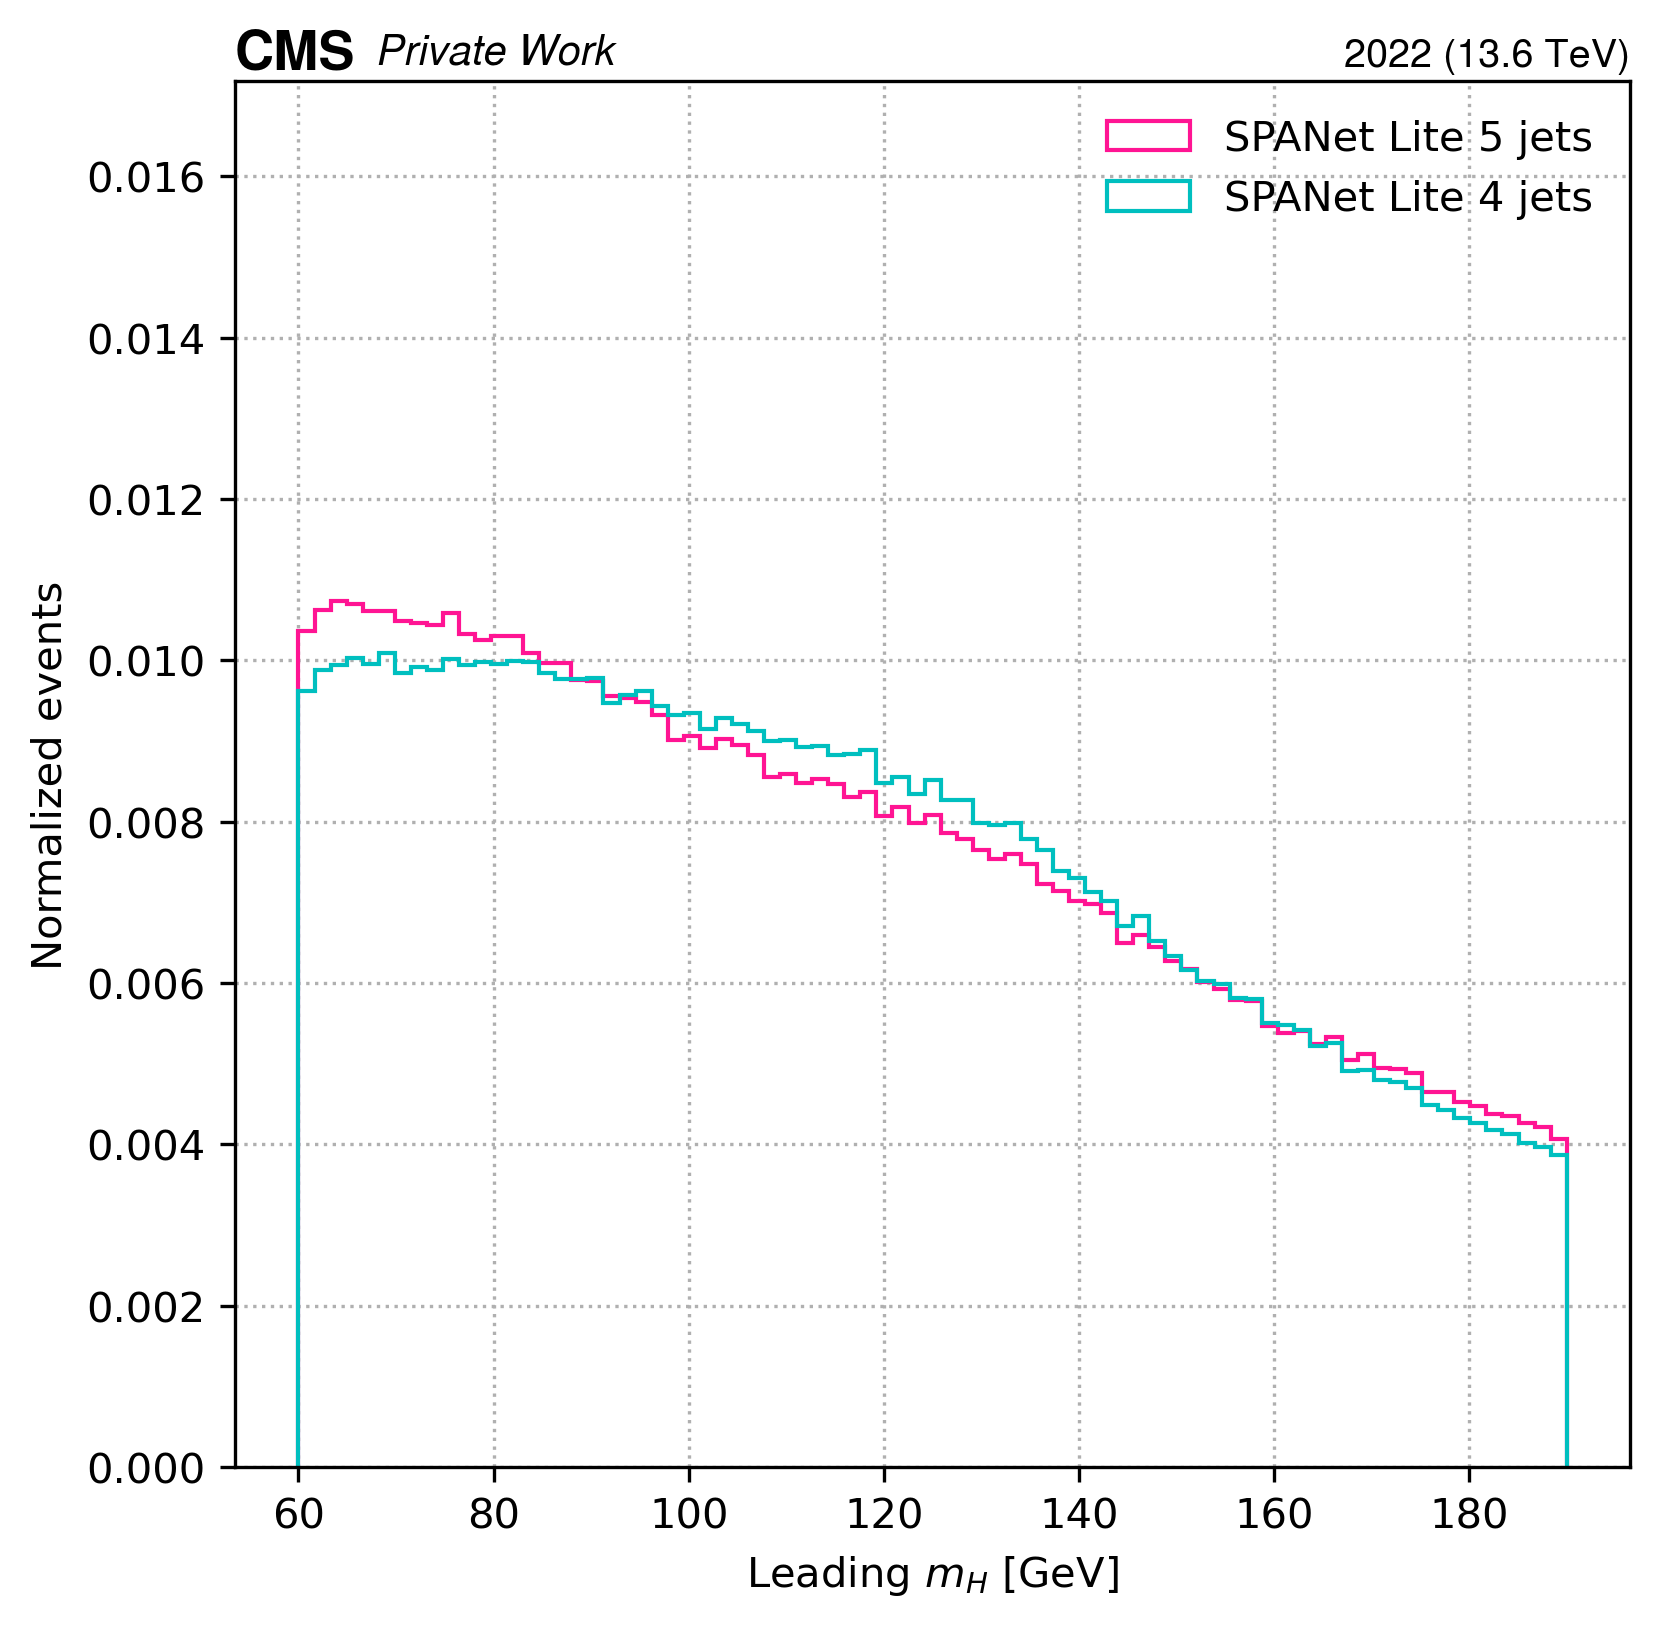
\includegraphics[width=0.6\linewidth]{Images/6.Improving/Mass sculpting/lead h sculpting.png}
    \caption{Distribution of the leading Higgs mass after the evaluation of the best performing models defined in Section \ref{subsection: results on the trainings} on 2b data.}
    \label{fig: 1D mass sculpting leading}
\end{figure}

\begin{figure}[hbt]
    \centering
    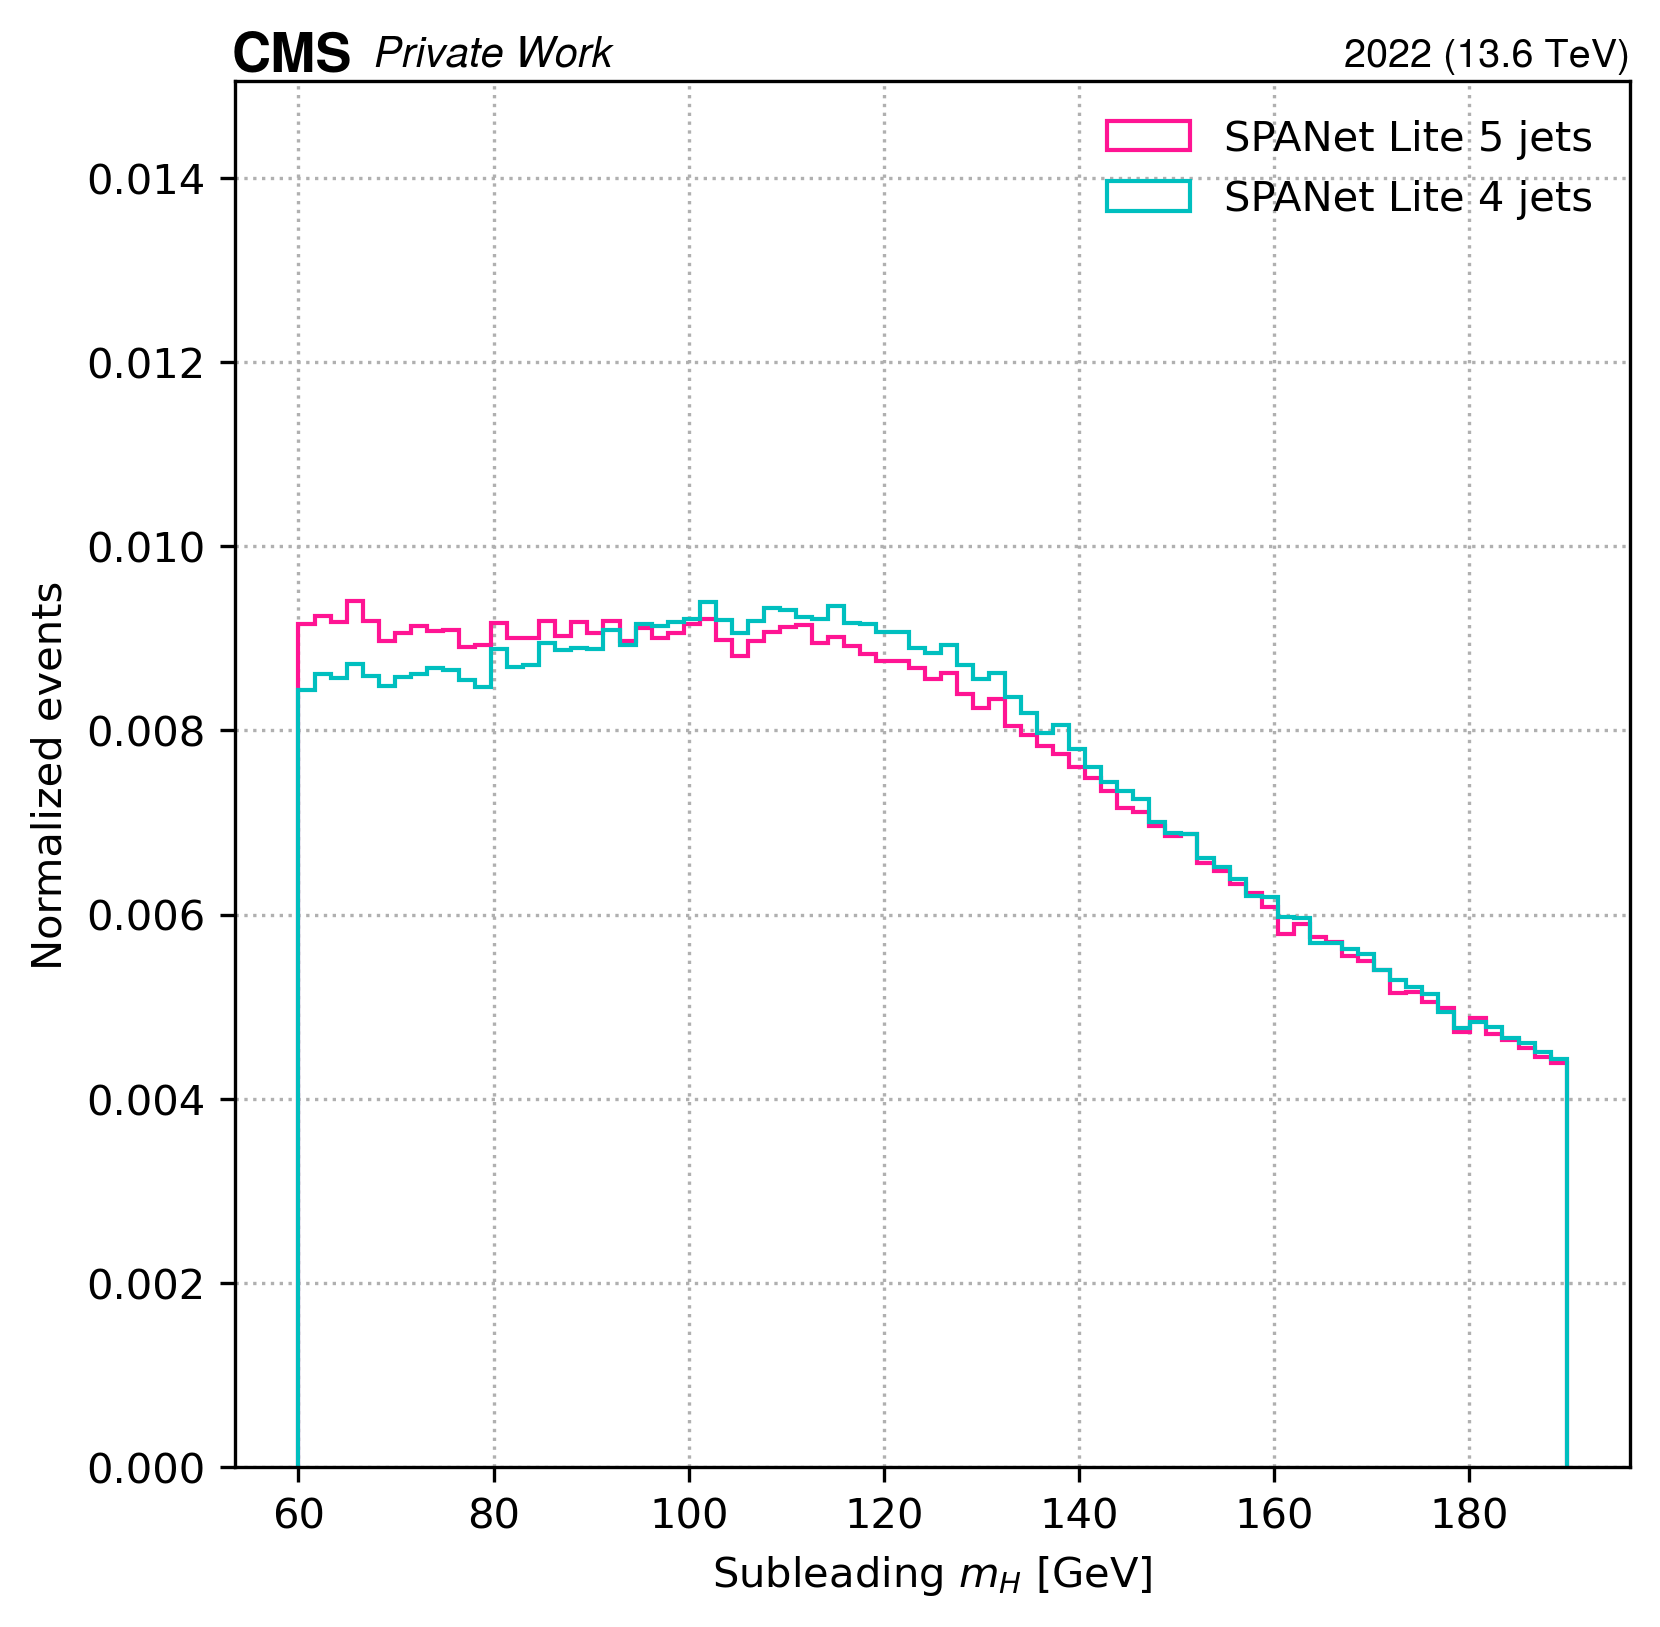
\includegraphics[width=0.6\linewidth]{Images/6.Improving/Mass sculpting/subleading h sculpting.png}
    \caption{Distribution of the subleading Higgs mass after the evaluation of the best performing models defined in Section \ref{subsection: results on the trainings} on 2b data.}
    \label{fig: 1D mass sculpting subleading}
\end{figure}

%The next question that arises when performing these tests, is that after performing several trainings with 5 jets, we observed a variability in the results, which is why, we decided to delve onto the variability of these trainings.

\clearpage

\subsection{Studies for the SPANet training variability} \label{subsection: pairing variability}

After performing several trainings with 5 jets, a variability is observed in the results, therefore a study regarding the model variability of the SPANet trainings is presented in this section. We define the model variability that will be tested in this section as the variability of our training with respect to the validation accuracy defined in Section \ref{section: spanet architecture}.

In order to assess the model variability, several trainings of the same model are performed fixing the seed to randomly initialize the weights. As a first test to address this variability issue, in addition to fixing the weights, we verify if the Pytorch version used for the training impacts the training variability. Three different trainings fixing the seeds to 0, 1, and 2 are performed for three different versions of Pytorch. We conclude that the variability is independent of the version we use when we fix the seed to initialize the weights. Therefore, for future trainings the latest version (2.2.2) is used. As a next step, 26 different trainings with 26 different seeds are performed to observe the variability. The results are shown in Figure \ref{fig: 5j variability}, where the validation accuracy for each training as a function of the batch size is shown. We observe that the validation accuracy clusters around two different values: 96.6\% and 94.5\%. Around each value, there is a spread of around 0.3\%. Therefore, a large variability of the model ($\sim$2\%) is observed. In order to assess this feature, the hyper-parameters of the training are modified to mitigate the intrinsic training variability assessed by checking the validation accuracy spread as a function of the batch size.

\begin{figure}[hbt]
    \centering
    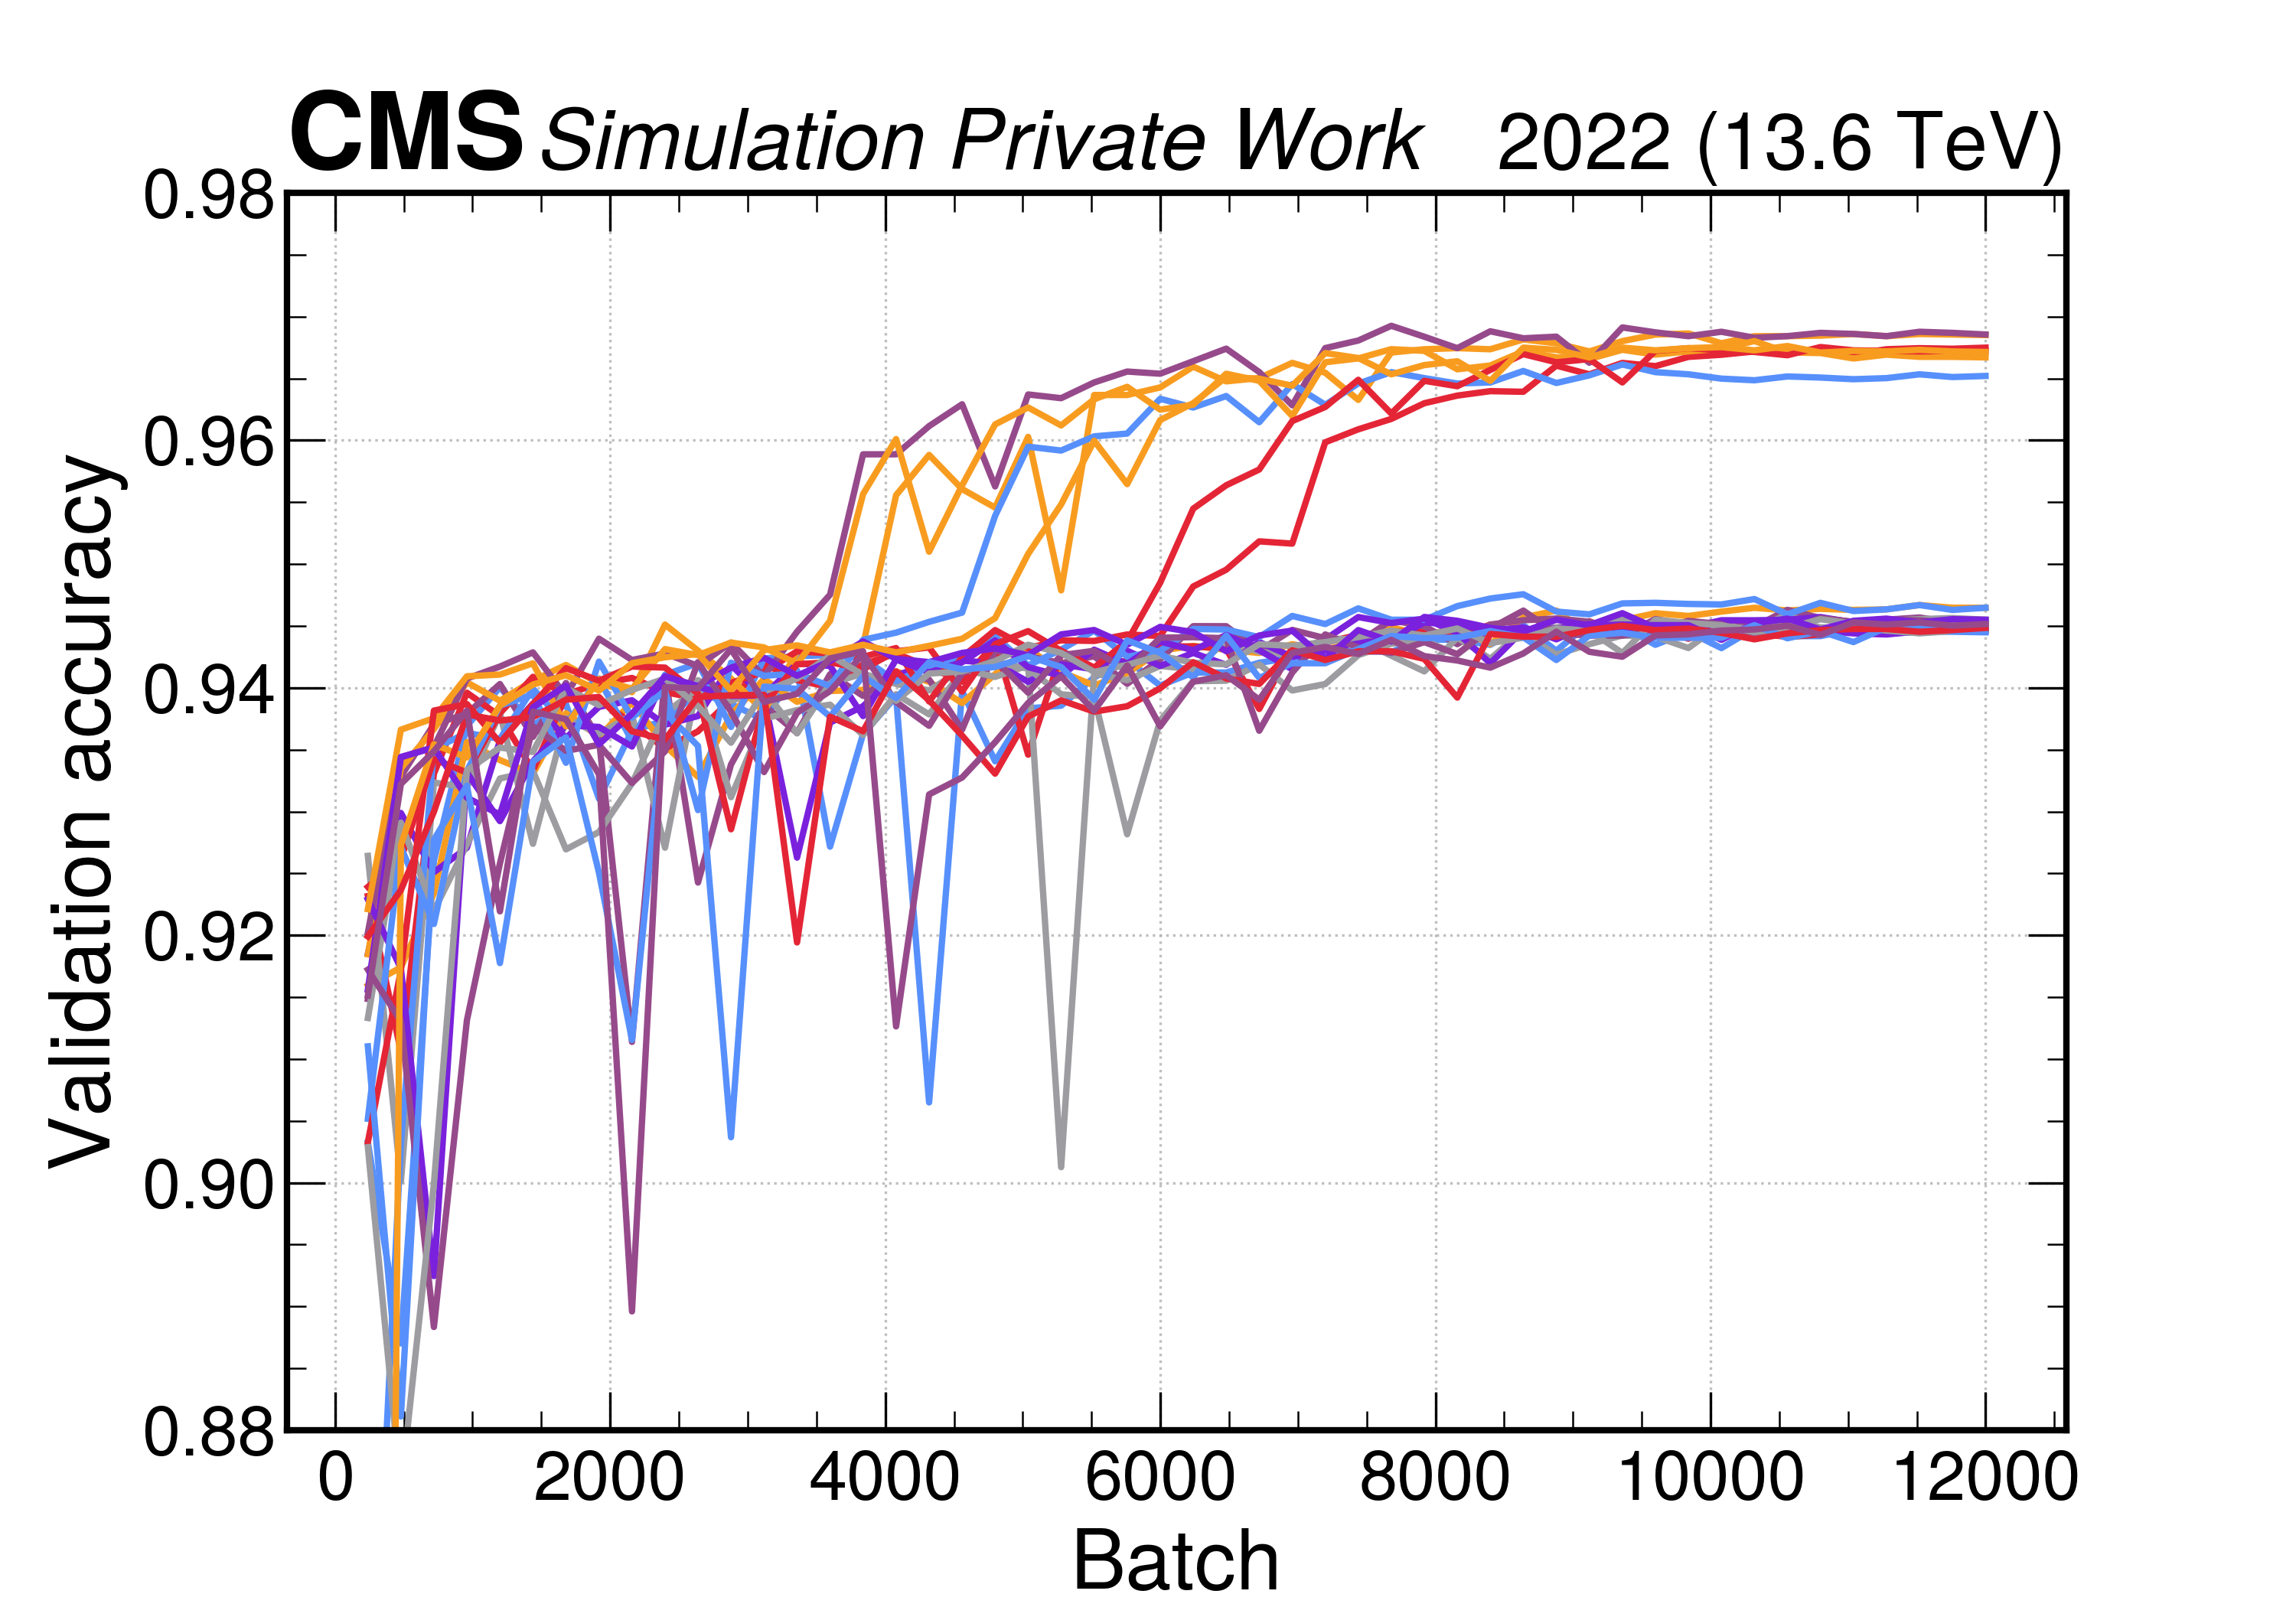
\includegraphics[scale=0.1]{Images/6.Improving/Variability Study/5 jets variability study.png}
    \caption{Variability of the validation accuracy as a function of the batch size of the training using 5 jets as inputs \pt regressed and Lite model parameters defined in Table \ref{table:5 jets trainings}.}
    \label{fig: 5j variability}
\end{figure}

In Table \ref{table:comparison_models}, the hyper-parameters of the Lite model are defined. Table \ref{table: variation hyperpaparm} shows the parameters of this model we aim to modify to mitigate the variability of our training. We will start by modifying the learning rate. The smaller the learning rate (LR), the more stable the model, therefore, the decrease in the value of the LR is tested. Moreover, by modifying the LR warm-up cycles and rate cycles, instead of reaching the highest values of the learning rate after a few batches as shown in Figure \ref{fig: lr comp}, the LR starts from the highest value and decays linearly. The highest values that have been tested are shown in Table \ref{table: variation hyperpaparm}.

\begin{table}[hbt]
\centering
\begin{tabular}{|p{5cm}|p{4cm}|p{5cm}|}
 \hline
 Hyper-parameters  & Lite model & Test for stabilization \\
 \hline
 Learning rate & 0.00659 & $5\times 10^{-3}$, $10^{-3}$, $5\times 10^{-4}$, $10^{-4}$ \\
 \hline
 Learning rate warmup cycles & 1 & 0\\
 \hline
  Learning rate cycles & 1 & 0\\
 \hline
 Batch size & 2048 / 1024 & 2048/1024 \\
 \hline
 Number of epochs & 50/300 & 50/300 \\
 \hline
\end{tabular}
\caption{Variations of the hyperparameters to stabilize the model.}
\label{table: variation hyperpaparm}
\end{table}

After performing several trainings, we concluded that the most stable configuration is given by the learning rate $10^{-4}$. As shown in Table \ref{table: variation hyperpaparm}, the impact on the variability and the SPANet pairing efficiency when modifying the batch size and the number of epochs are also tested.

Figure \ref{fig: stable test} shows that when using the new hyperparameters (LR=$10^{-4}$) with a batch size of 2048 and 50 epochs all trainings cluster around 95.9-96.4\%, which corresponds to an approximate spread in the validation accuracy of 0.5\%. This variability is considered to be acceptable. Figure \ref{fig: stable test 1024} shows the training when using a batch size of 1024 instead of 2048. In this case, the trainings cluster around the 96\% but with a spread of 0.3\%. However, using a a batch size of 2048 allows us to have faster trainings, therefore, since the difference in the spread is not very significant, it is chosen to keep a batch size of 2048. 

\begin{figure}[hbt]
    \centering
    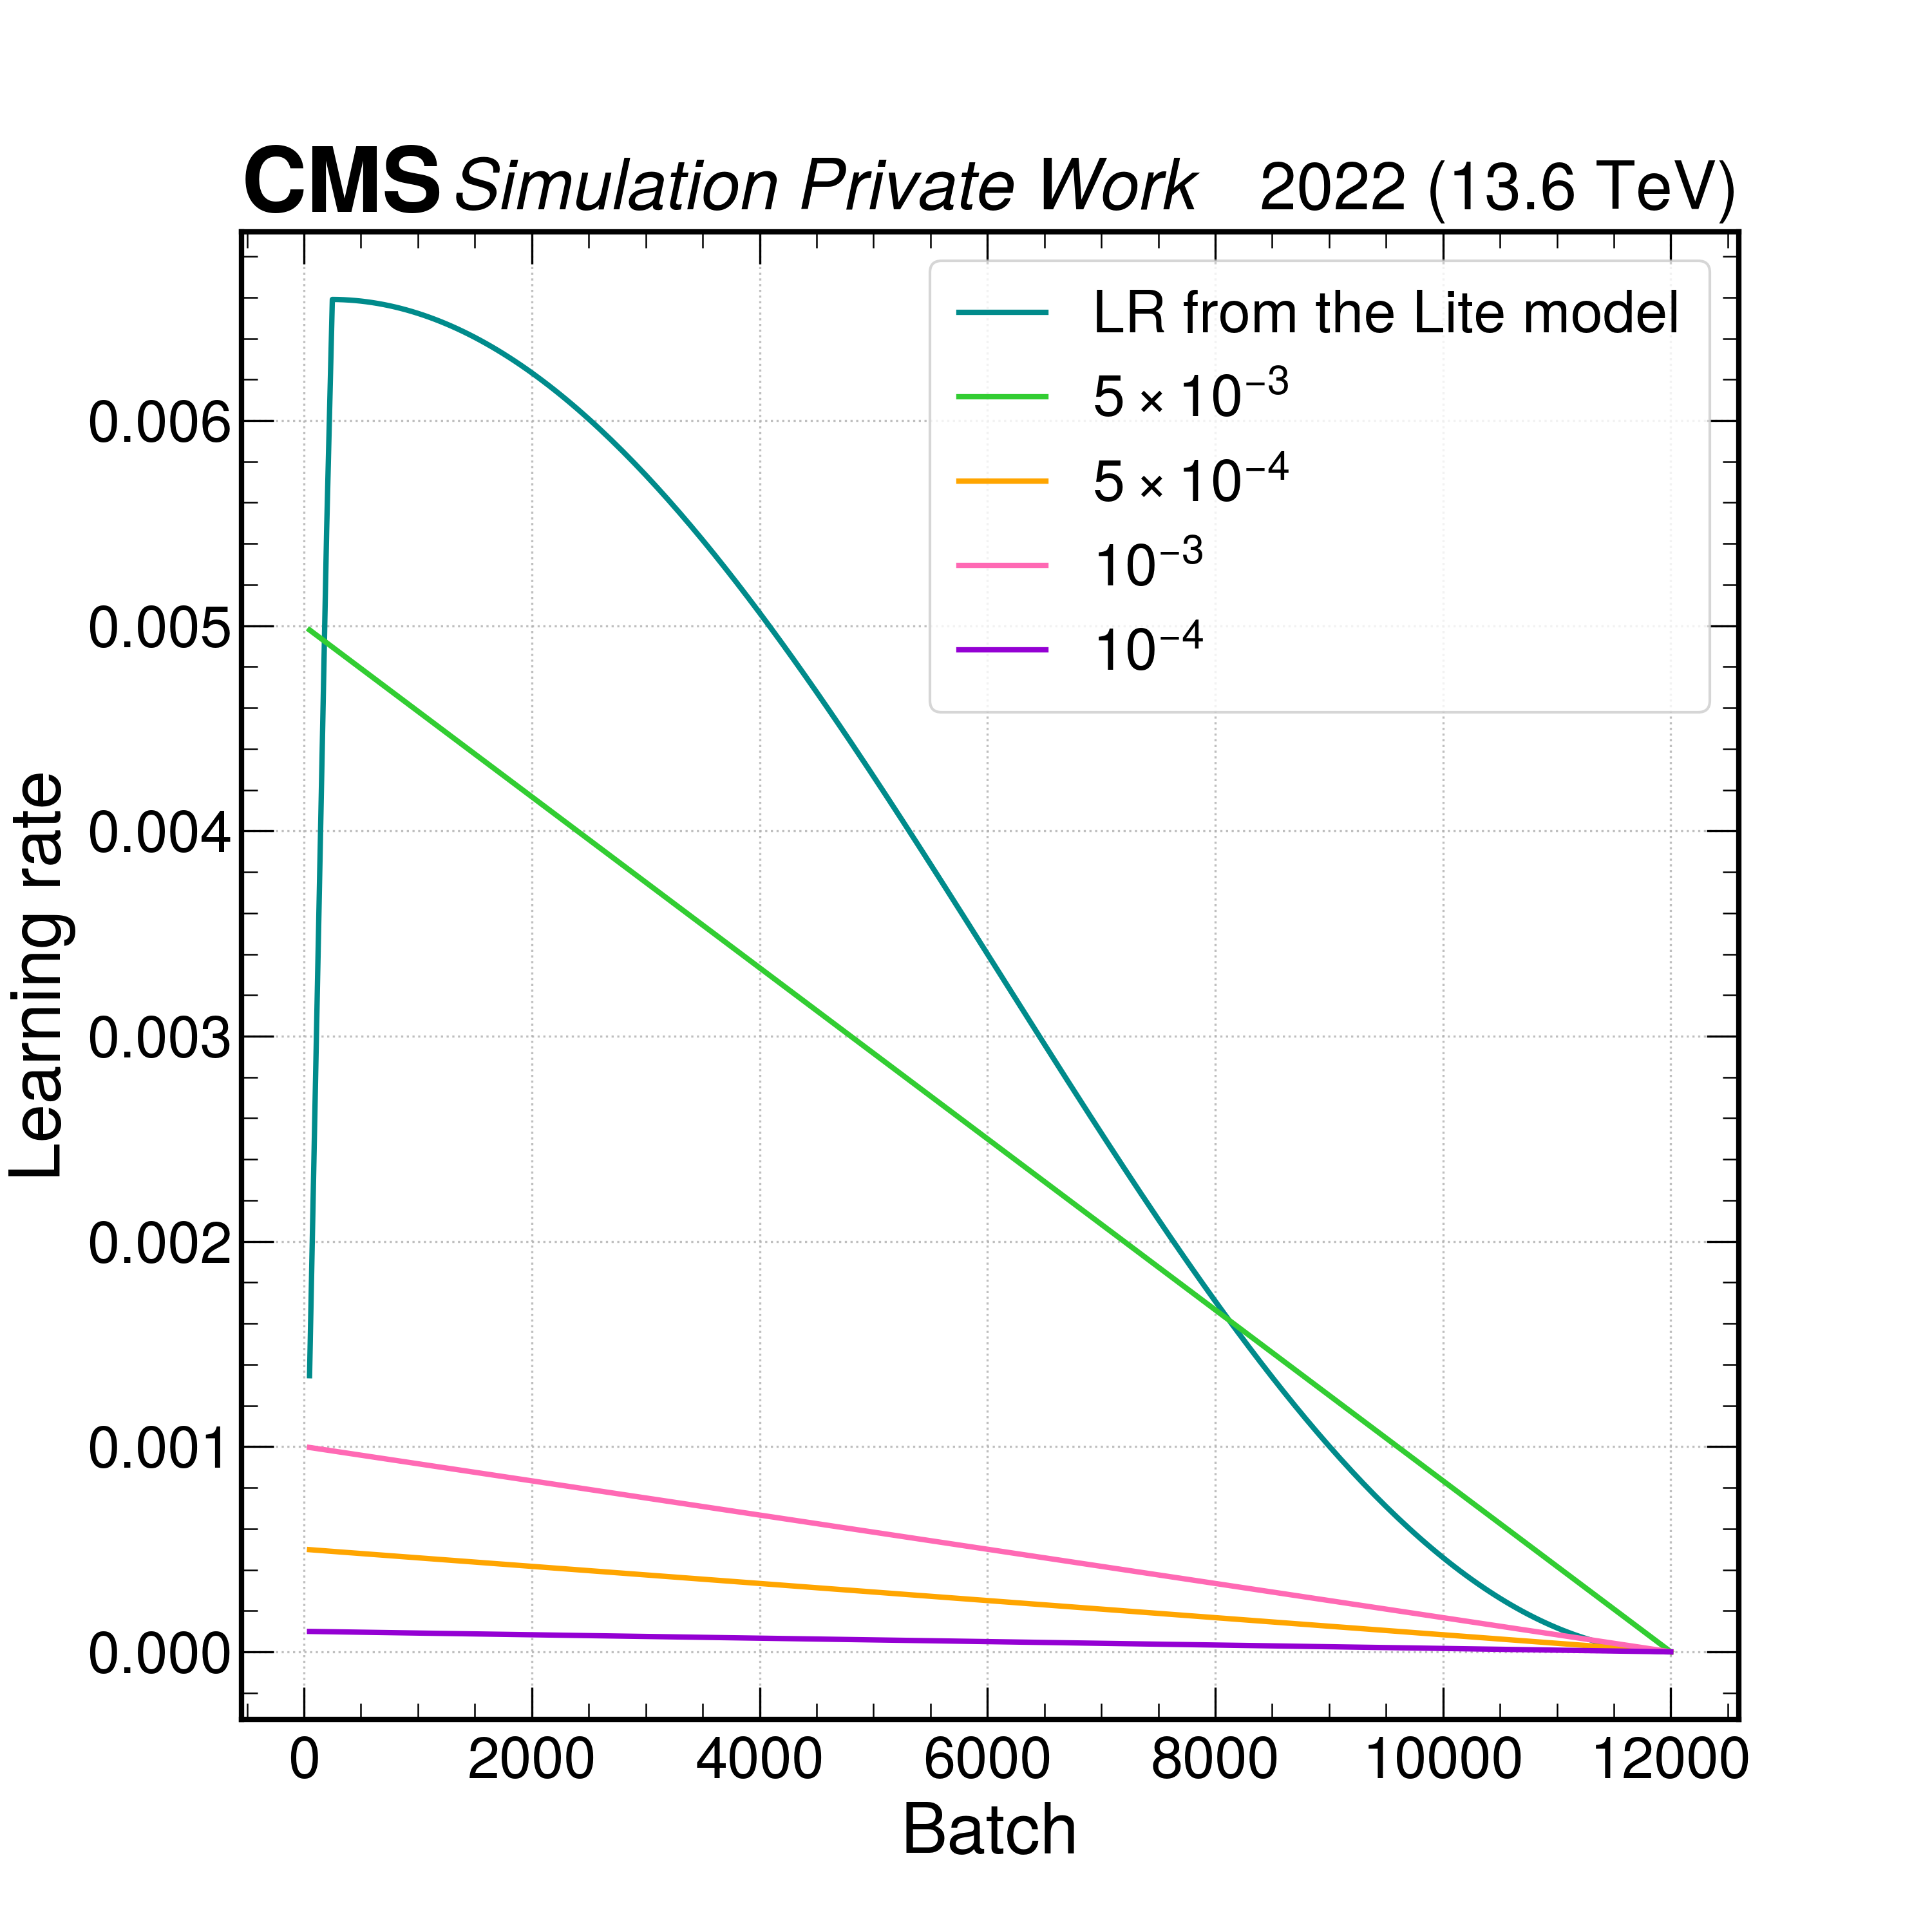
\includegraphics[width=0.6\linewidth]{Images/6.Improving/Variability Study/learning rate comp.png}
    \caption{Comparison of the learning rate (LR) used in the Lite model defined in Table \ref{table:comparison_models} (blue) to the learning rates presented in Table \ref{table: variation hyperpaparm}. The variations of the LR warm-up cycles as well as the cycles as described in Table \ref{table: variation hyperpaparm} explain the difference in the shape of the LR as a function of the batch size.}
    \label{fig: lr comp}
\end{figure}

\begin{figure}[hbt]
    \centering
    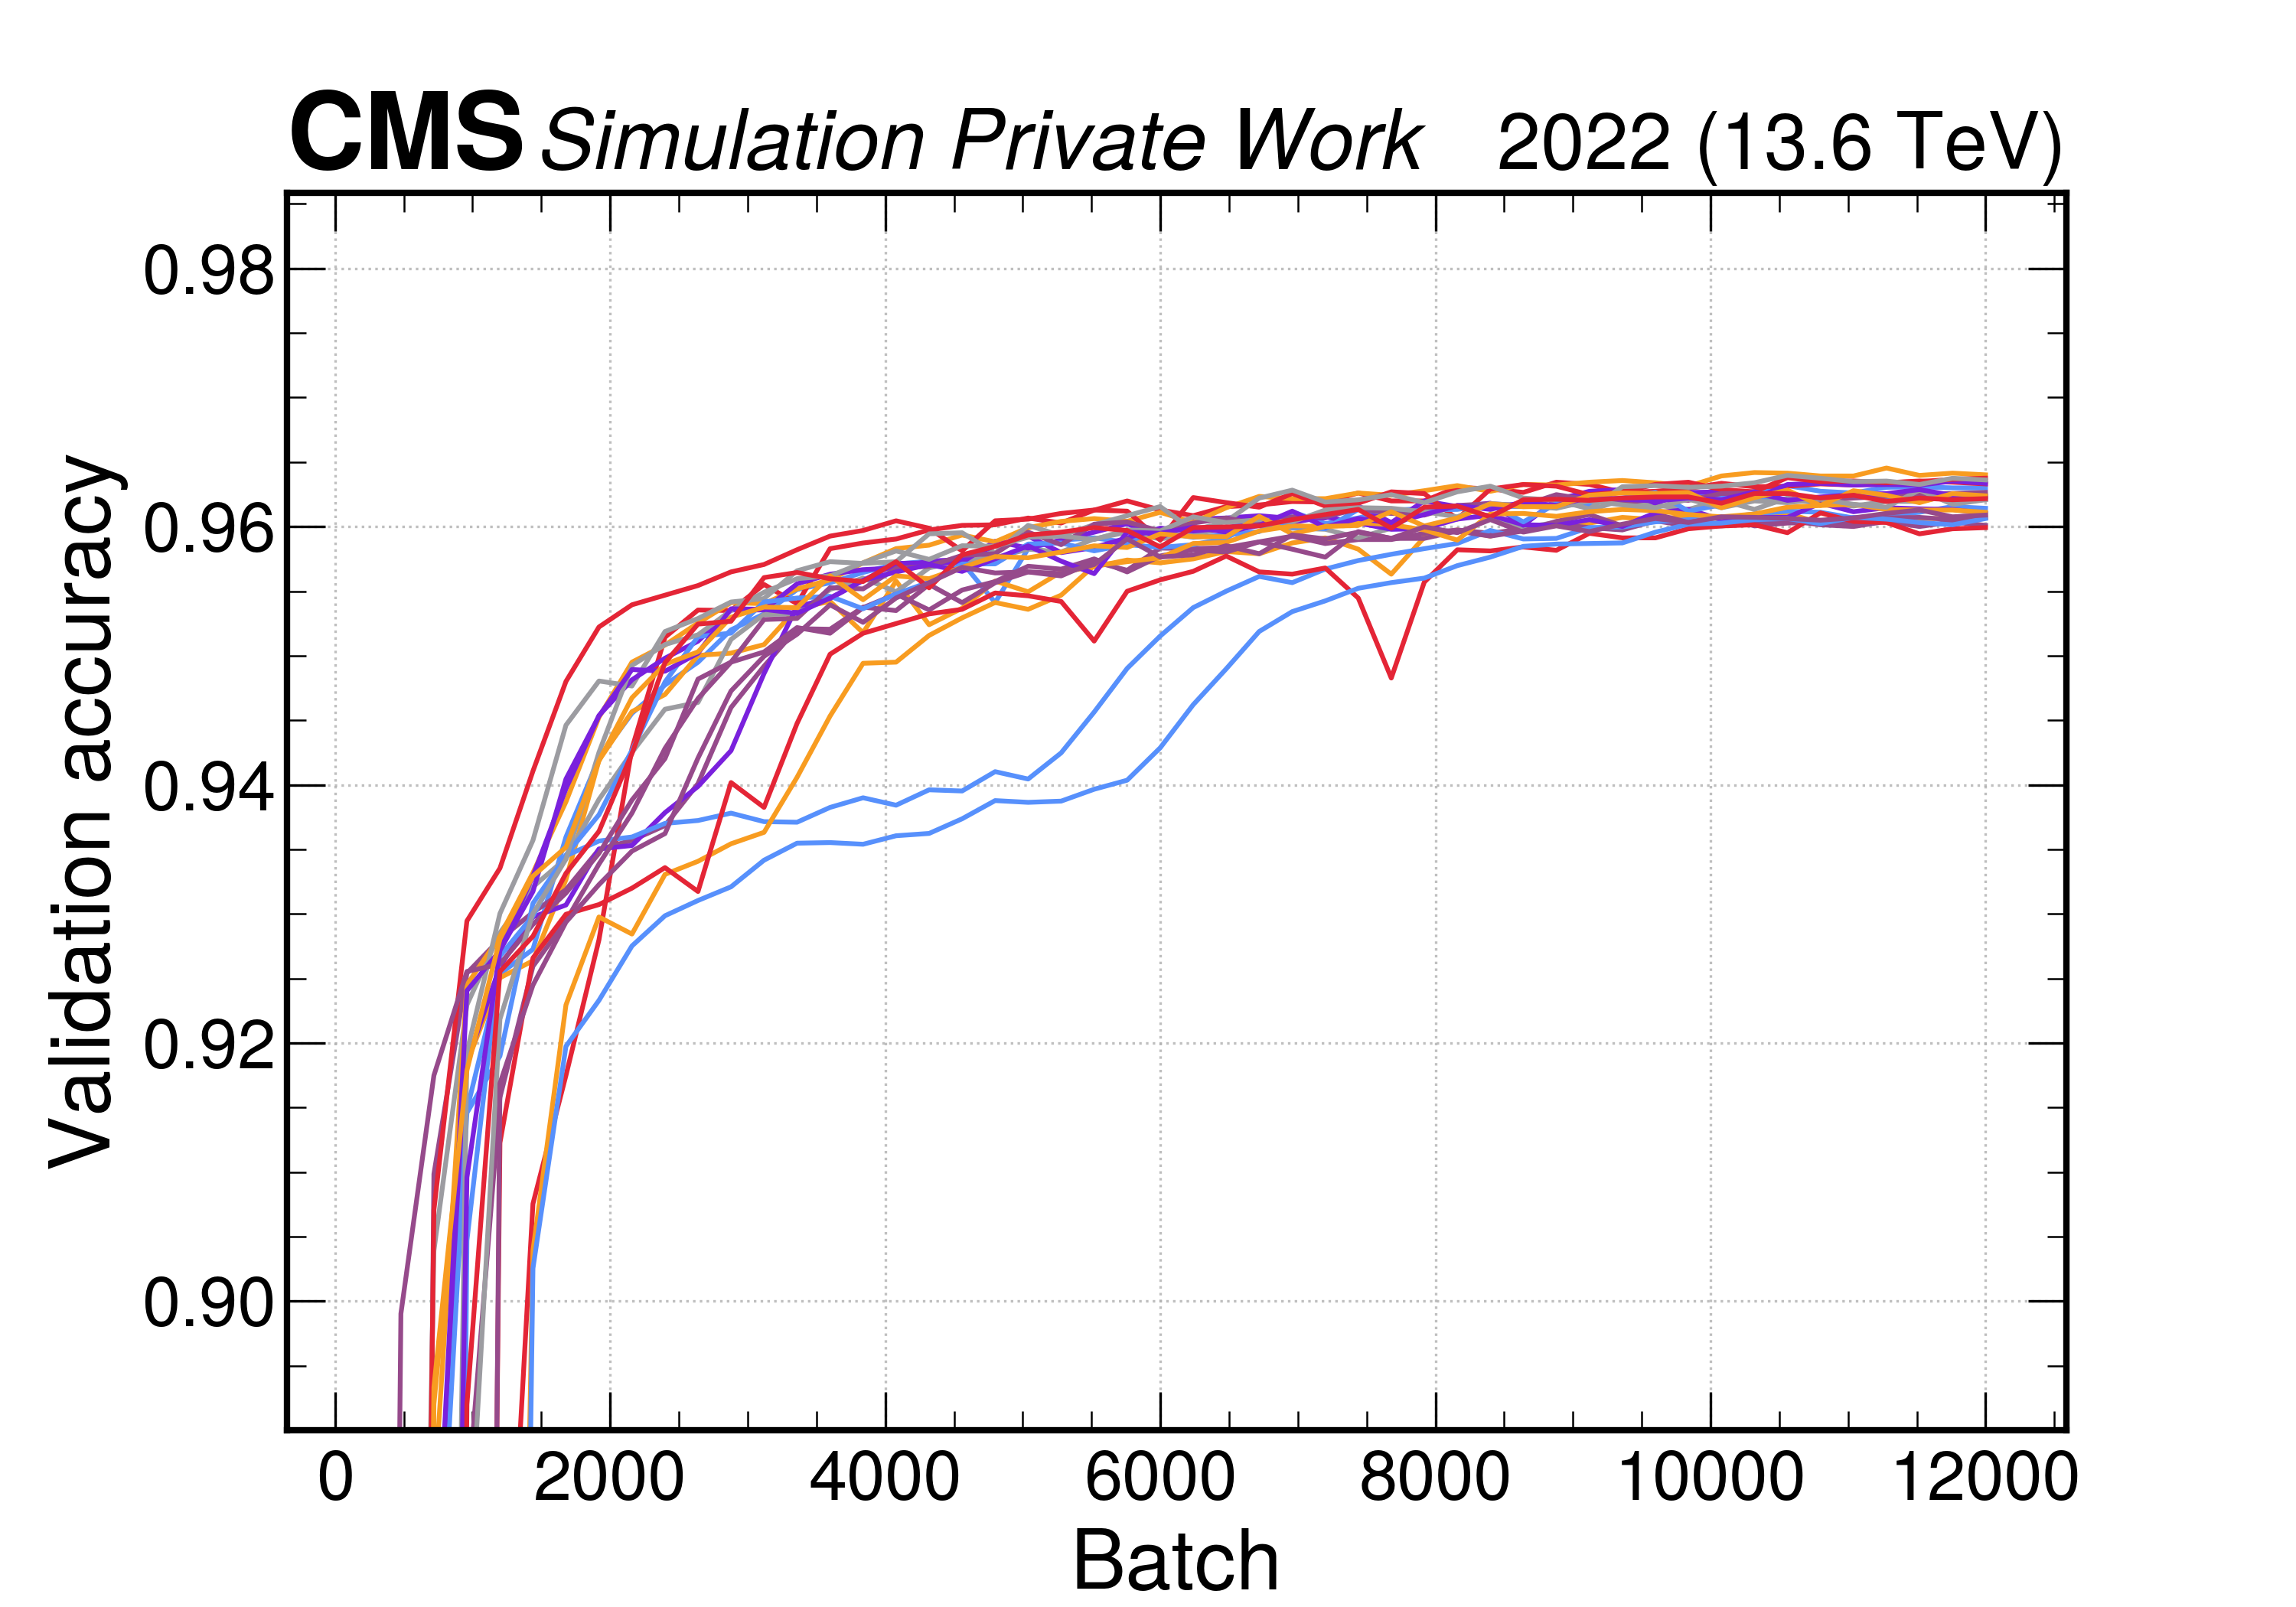
\includegraphics[width=0.7\linewidth]{Images/6.Improving/Variability Study/var 2048.png}
    \caption{Variability of the validation accuracy as a function of the batch size of the training with 5 jets as inputs \pt regressed, LR of $10^{-4}$, LR cycle and warm-up cycles equal to 0, a batch size of 2048 and 50 epochs}
    \label{fig: stable test}
\end{figure}

\begin{figure}[hbt]
    \centering
    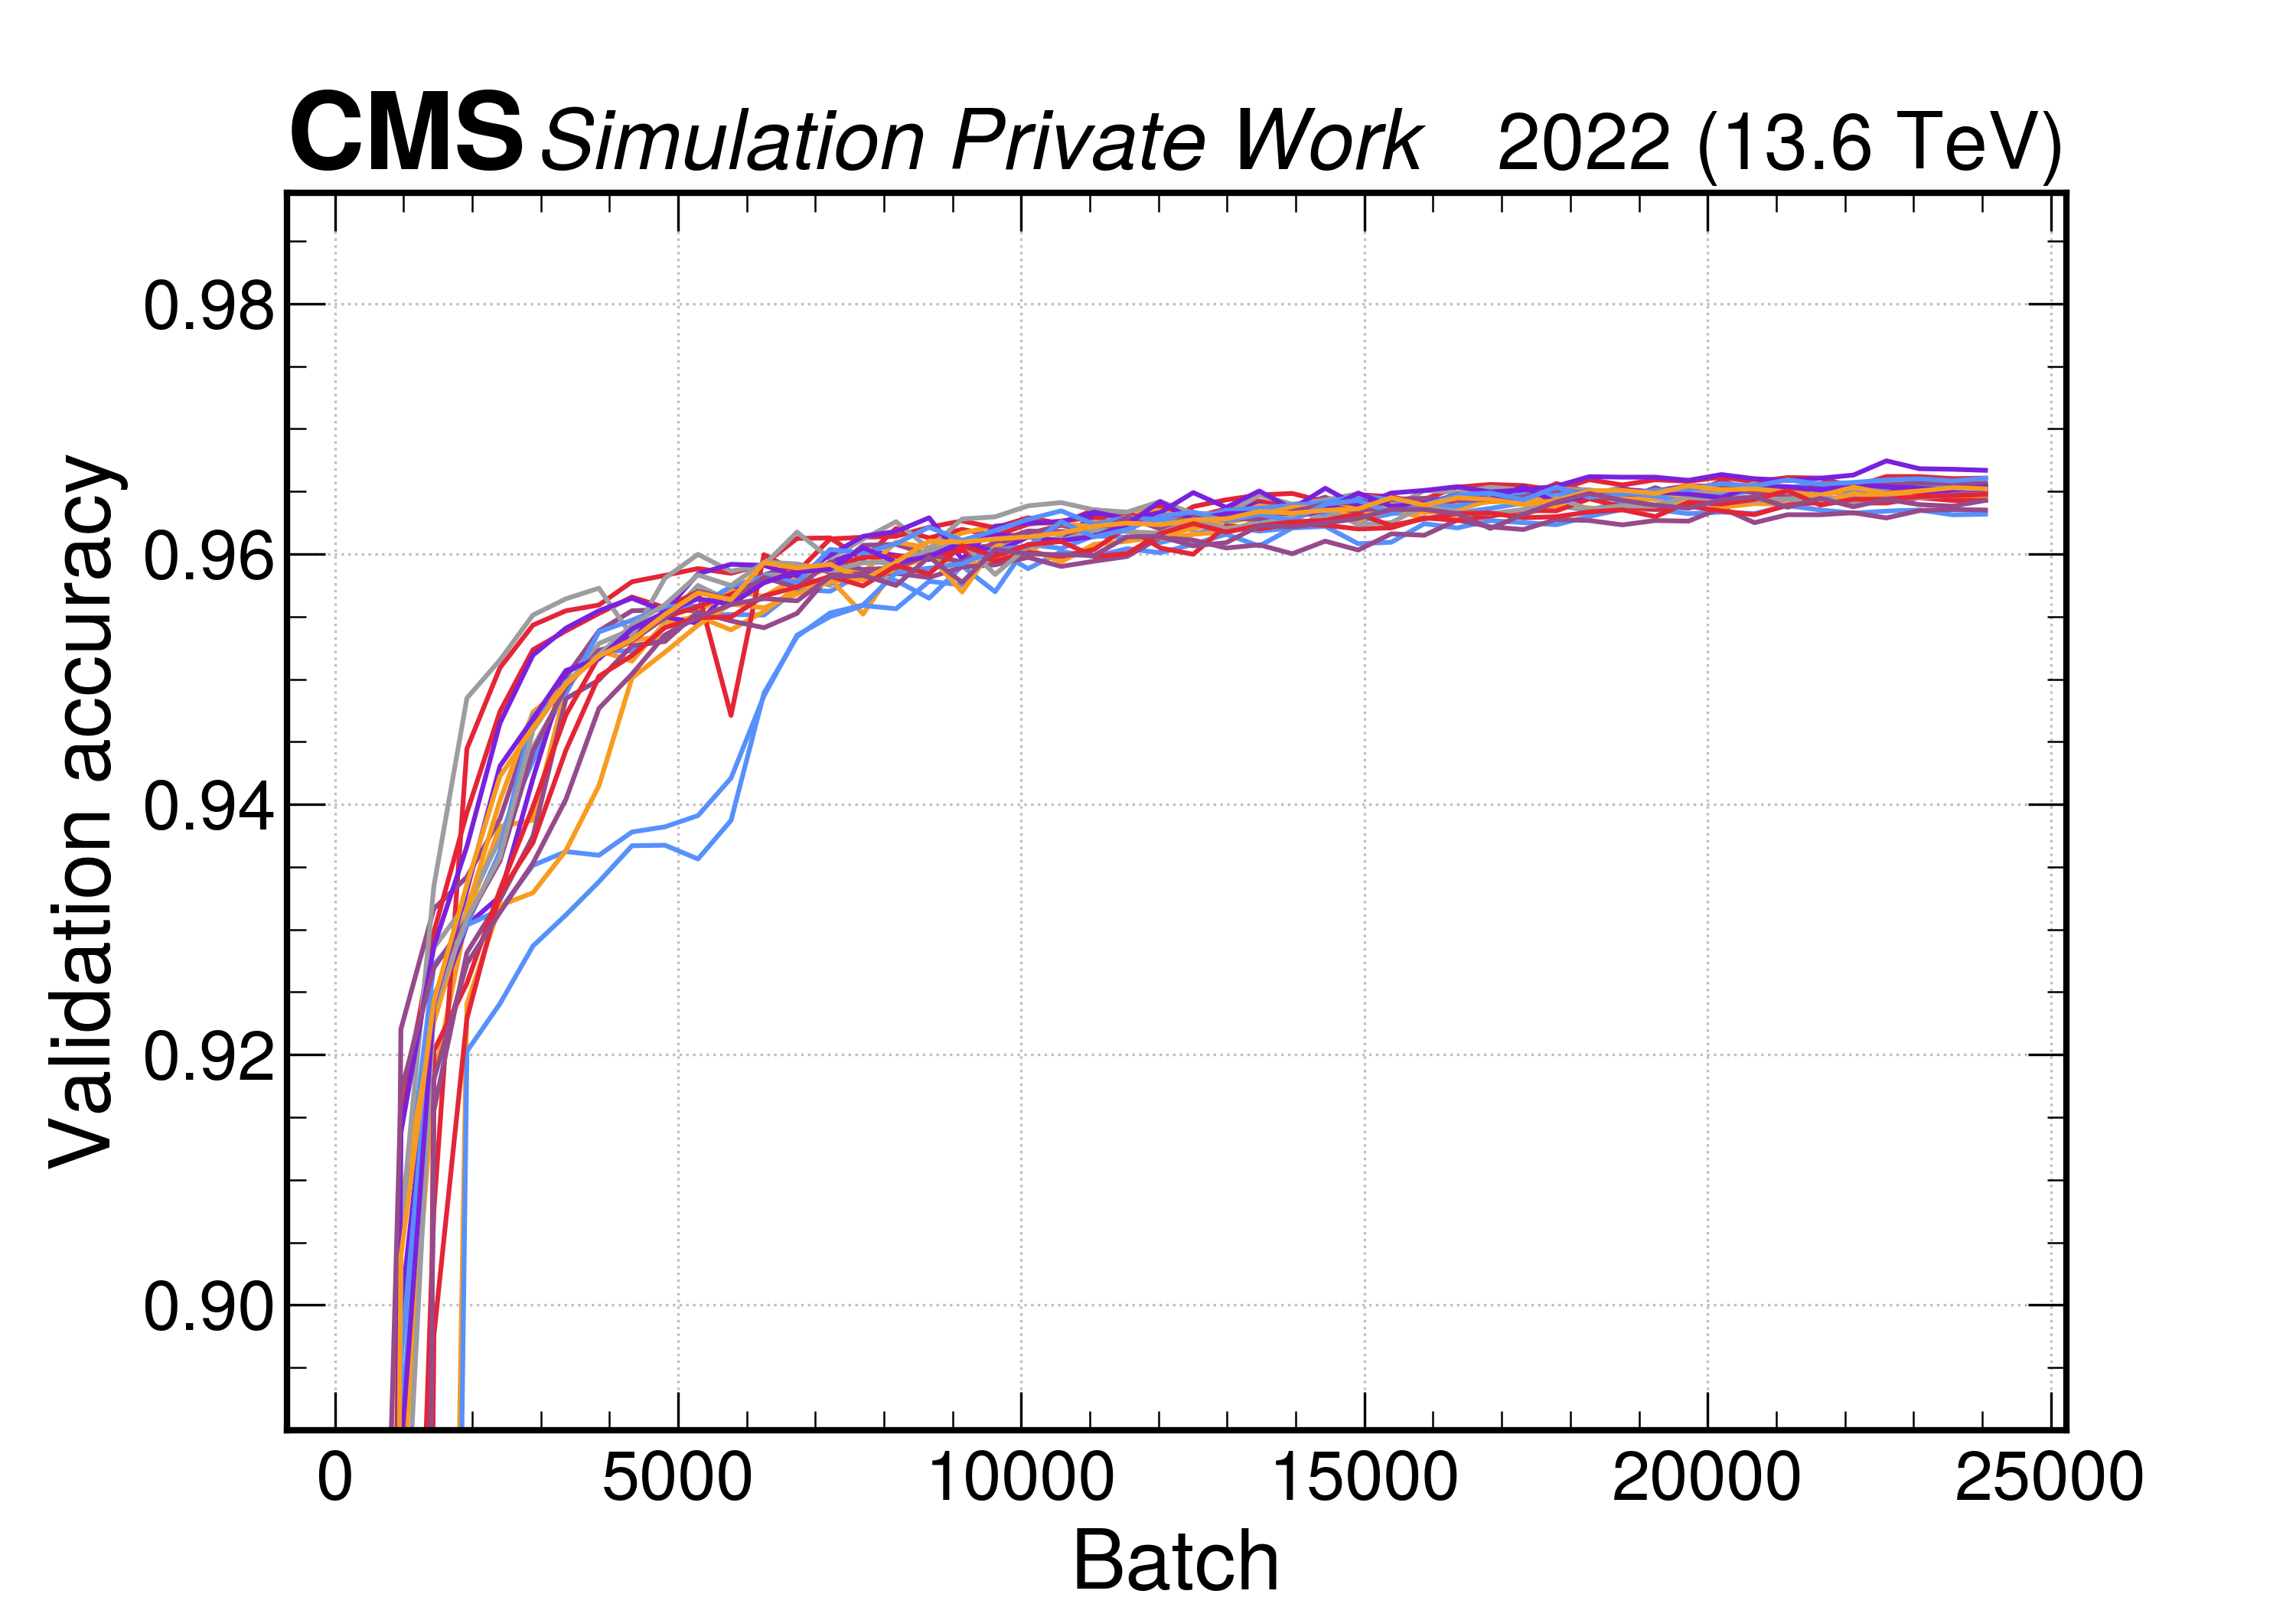
\includegraphics[width=0.7\linewidth]{Images/6.Improving/Variability Study/var 1024.png}
    \caption{Variability of the validation accuracy as a function of the batch size of the training with 5 jets as inputs \pt regressed, LR equal to $10^{-4}$, LR cycle and warm-up cycles equal to 0, a batch size of 1024 and 50 epochs}
    \label{fig: stable test 1024}
\end{figure}



Finally, the difference in the efficiency when varying the number of epochs is studied. Figure \ref{fig: epoch diff} shows that the validation accuracy is improved by around 0.4\% when using 300 epochs. In conclusion, after this study, the most stable and efficient configuration is given by the parameters shown in Table \ref{table: stable model}.

\begin{figure}[hbt]
    \centering
    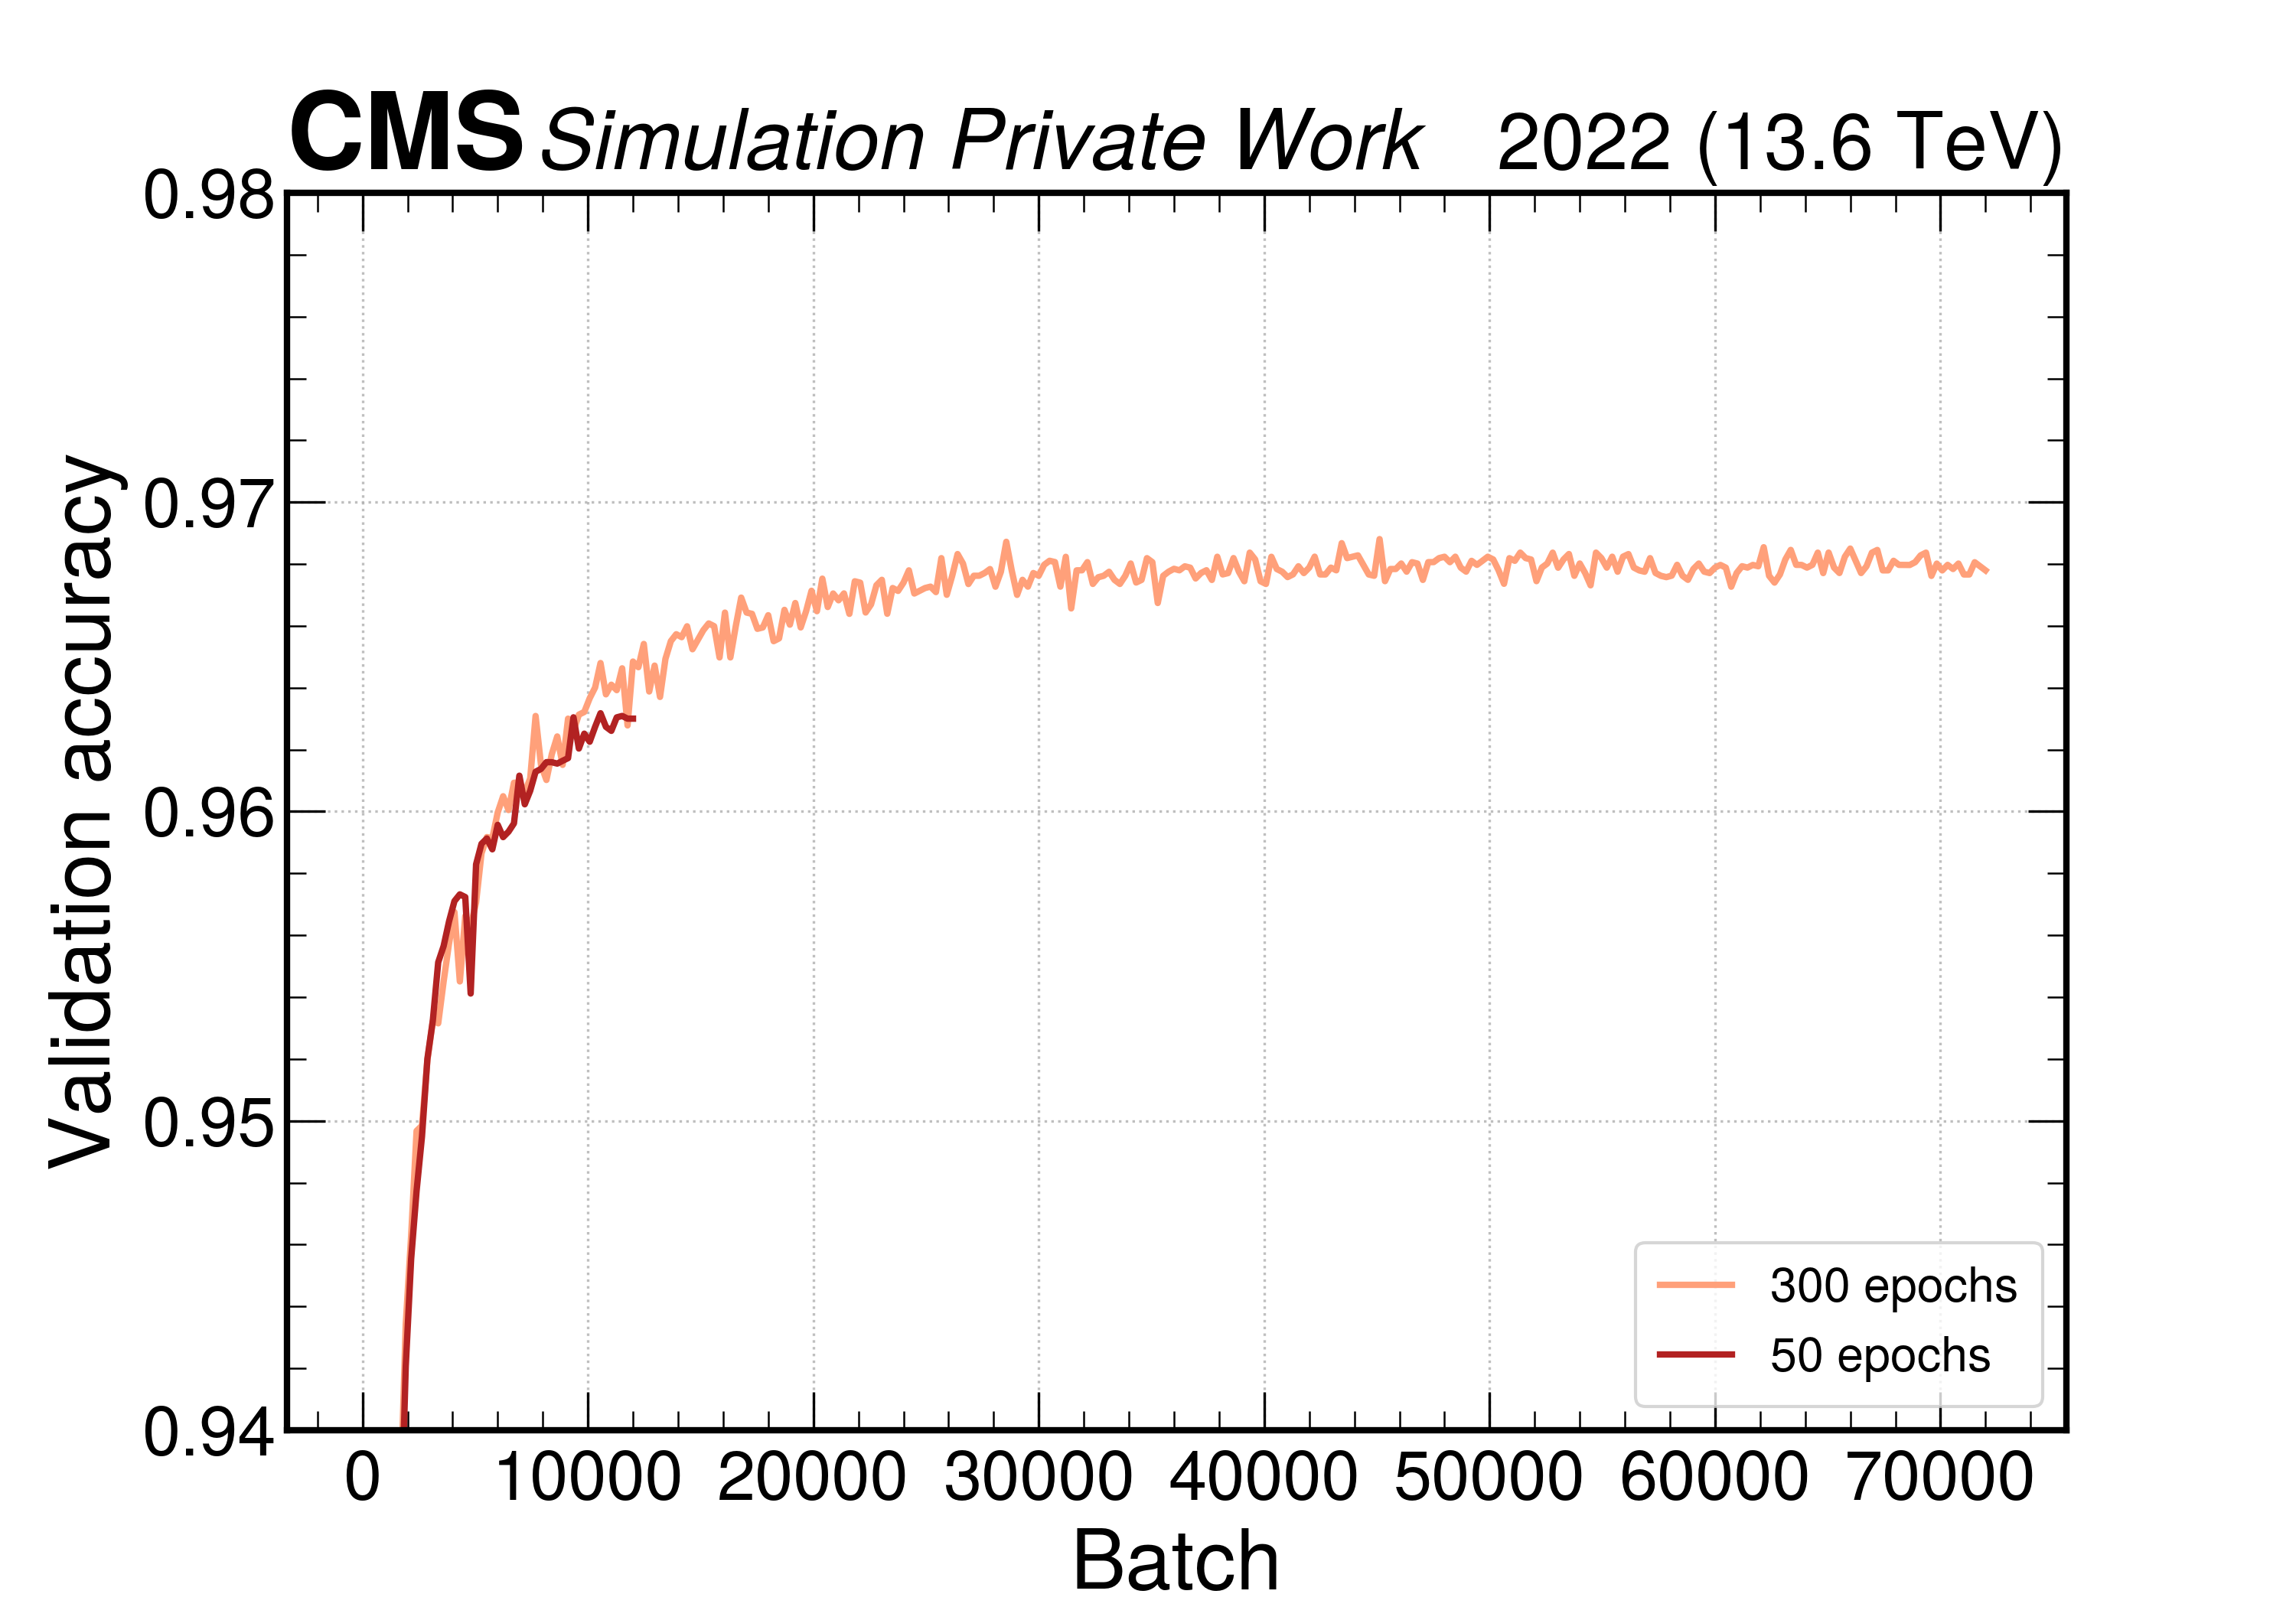
\includegraphics[width=0.7\linewidth]{Images/6.Improving/Variability Study/epoch comp.png}
    \caption{Comparison in the number of epochs of performance the training with 5 jets as inputs using our stable model}
    \label{fig: epoch diff}
\end{figure}

\begin{table}[hbt]
\centering
\begin{tabular}{|c|c|}
 \hline
 Parameters  & Stable model  \\
 \hline
 Learning rate &  $10^{-4}$ \\
 \hline
 Learning rate warmup cycles &  0\\
 \hline
  Learning rate cycles & 0\\
 \hline
 Batch size & 2048 \\
 \hline
 Number of epochs & 300 \\
 \hline
\end{tabular}
\caption{Configuration for the Stable model}
\label{table: stable model}
\end{table}


\newpage

\subsection{Grid search} \label{subsection: grid search}

In the following sections the 5 jet \pt regressed model using the Stable model hyper-parameters defined in Table \ref{table: stable model} will be used for the trainings. In order to increase the performance of the 5 jets \pt regressed Stable model, a grid search is performed, thanks to which we should find the optimal configuration of hyper-parameters.

In order to do so, the features of the Stable model are used and the hyperparameters presented in Table \ref{table: parameters for the grid search} are changed, as they are the default ones proposed by SPANet for the tuning. 
However, contrary to what is specified in Table \ref{table: stable model} for this grid search we use 50 epochs, as the difference in performance compared to 300 epochs showed in Figure \ref{fig: epoch diff} is very small, and the trainings are completed faster.
As shown in Table \ref{table: parameters for the grid search}, we give several possible values for the hyperparameters and then several trainings are performed combining them differently.
For the first three, SPANet chooses between a value among the ones reported in Table \ref{table: parameters for the grid search}, whereas for the L2 Penalty the network can choose any value in the range [1e-5 : 1e-3] (in log scale).
The final outcome of this search is the combination of hyperparameters that provides the best performance. The optimal hyper-parameters obtained by this grid search are reported in Table \ref{table: parameters for the grid search} as well.

\begin{table}[hbt]
   \centering
   \begin{tabular}{|c|c|c|}
   \hline
    Hyper-parameters  &  Tested values & Optimal choice \\
    \hline
    Hidden dimension  &  \{32, 64, 96\} & 96 \\
    \hline
   Number of encoder layers & \{5, 6, 7, 8\} & 5 \\
    \hline
    Number of branch embedding layers &  \{1, 2, 3, 4\} & 3 \\
    \hline
     Number of branch encoder layers & 4 & 4\\
    \hline
    Number of regression layers & 3 & 3 \\
    \hline
    Number of classification layers & 1 & 1\\
    \hline
    Focal gamma & 0.0 & 0.0 \\
    \hline
    L2 Penalty & [1e-5 : 1e-3] & $7.3\times 10^{-4}$ \\
    \hline
   \end{tabular}
   \caption{Hyper-parameters modified during the grid search to increase the performance of the SPANet network. The second column shows the possible values that are chosen by SPANet during the search. The last column shows the final optimal hyper-parameters determined by the grid search.}
   \label{table: parameters for the grid search}
\end{table}

\newpage
By using these new hyperparameters the optimal model used for the analysis has 5.1 M trainable parameters compared to 0.5 M in the Stable model. 
As shown in Figure \ref{fig: comp grid search}, by using these new hyperparameters, 
there is no significant increase in the performance compared to the Stable model performance. 
Hence, in the following, the hyperparameters from the Stable Model are used.

\begin{figure}[hbt]
    \centering
    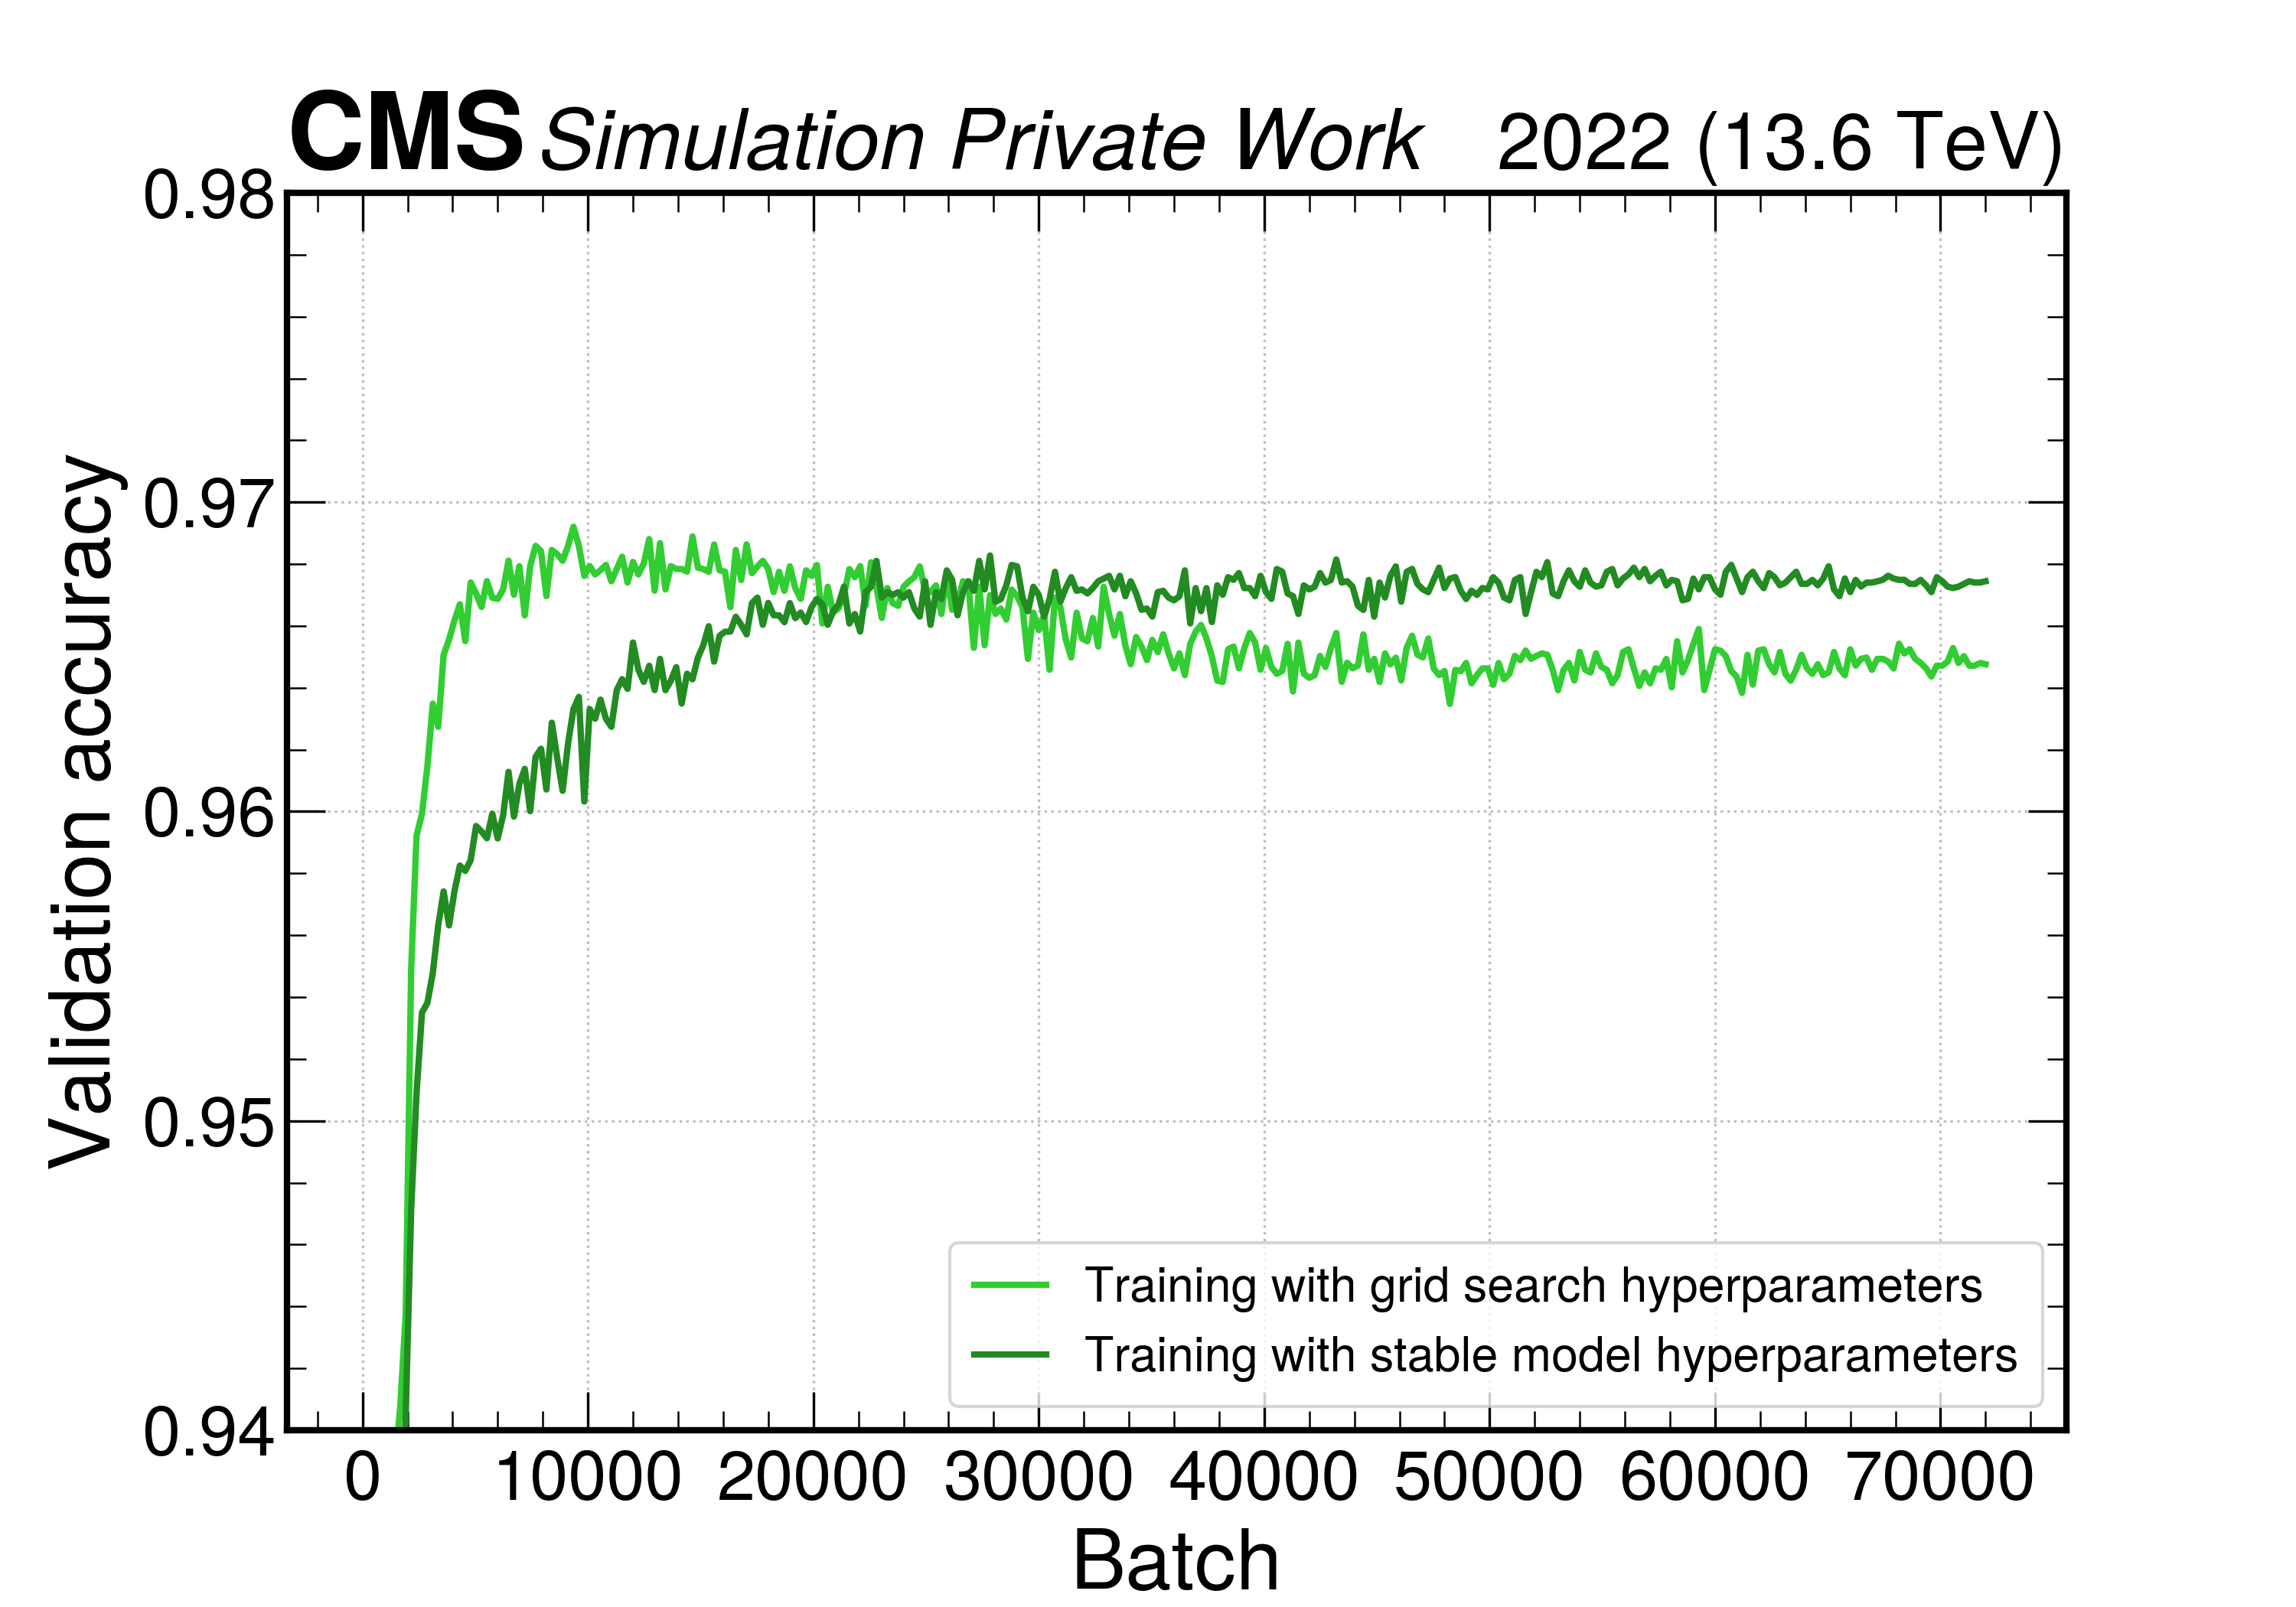
\includegraphics[width=0.6\linewidth]{Images/6.Improving/Grid search/grid search.png}
    \caption{Comparison of the training using the Stable model parameters and the optimal hyperparameters set given by the grid search.}
    \label{fig: comp grid search}
\end{figure}

%Do i mention other traiinngs done by Mathieu?

\clearpage

\subsection{Introducing \kl in the trainings} \label{subsection: kl}

As explained in Section \ref{section: HH4b}, by measuring the di-Higgs production we are aiming to study 
the Higgs boson self-coupling parameter $\lambda$. However, when \kl (defined in Section \ref{section: HH4b}) varies, the kinematics 
of the signal process change and therefore the distributions of some of our observables. Figure \ref{fig: mhh dist} shows an example of the $m_{HH}$ distribution for different \kl. Therefore, it is important to add this feature to the SPANet trainings. 
In order to do so, we employ several signal samples with different values of $\kappa_\lambda 
\in \{-2.0, -1.0, 0.0, 0.5, 1.0, 1.5, 2.0, 2.45, 3.0, 3.5, 4.0, 5.0\}$. 

%(Do I specify that we performed a validation study between the private and public samples?)

\begin{figure}[hbt]
    \centering
    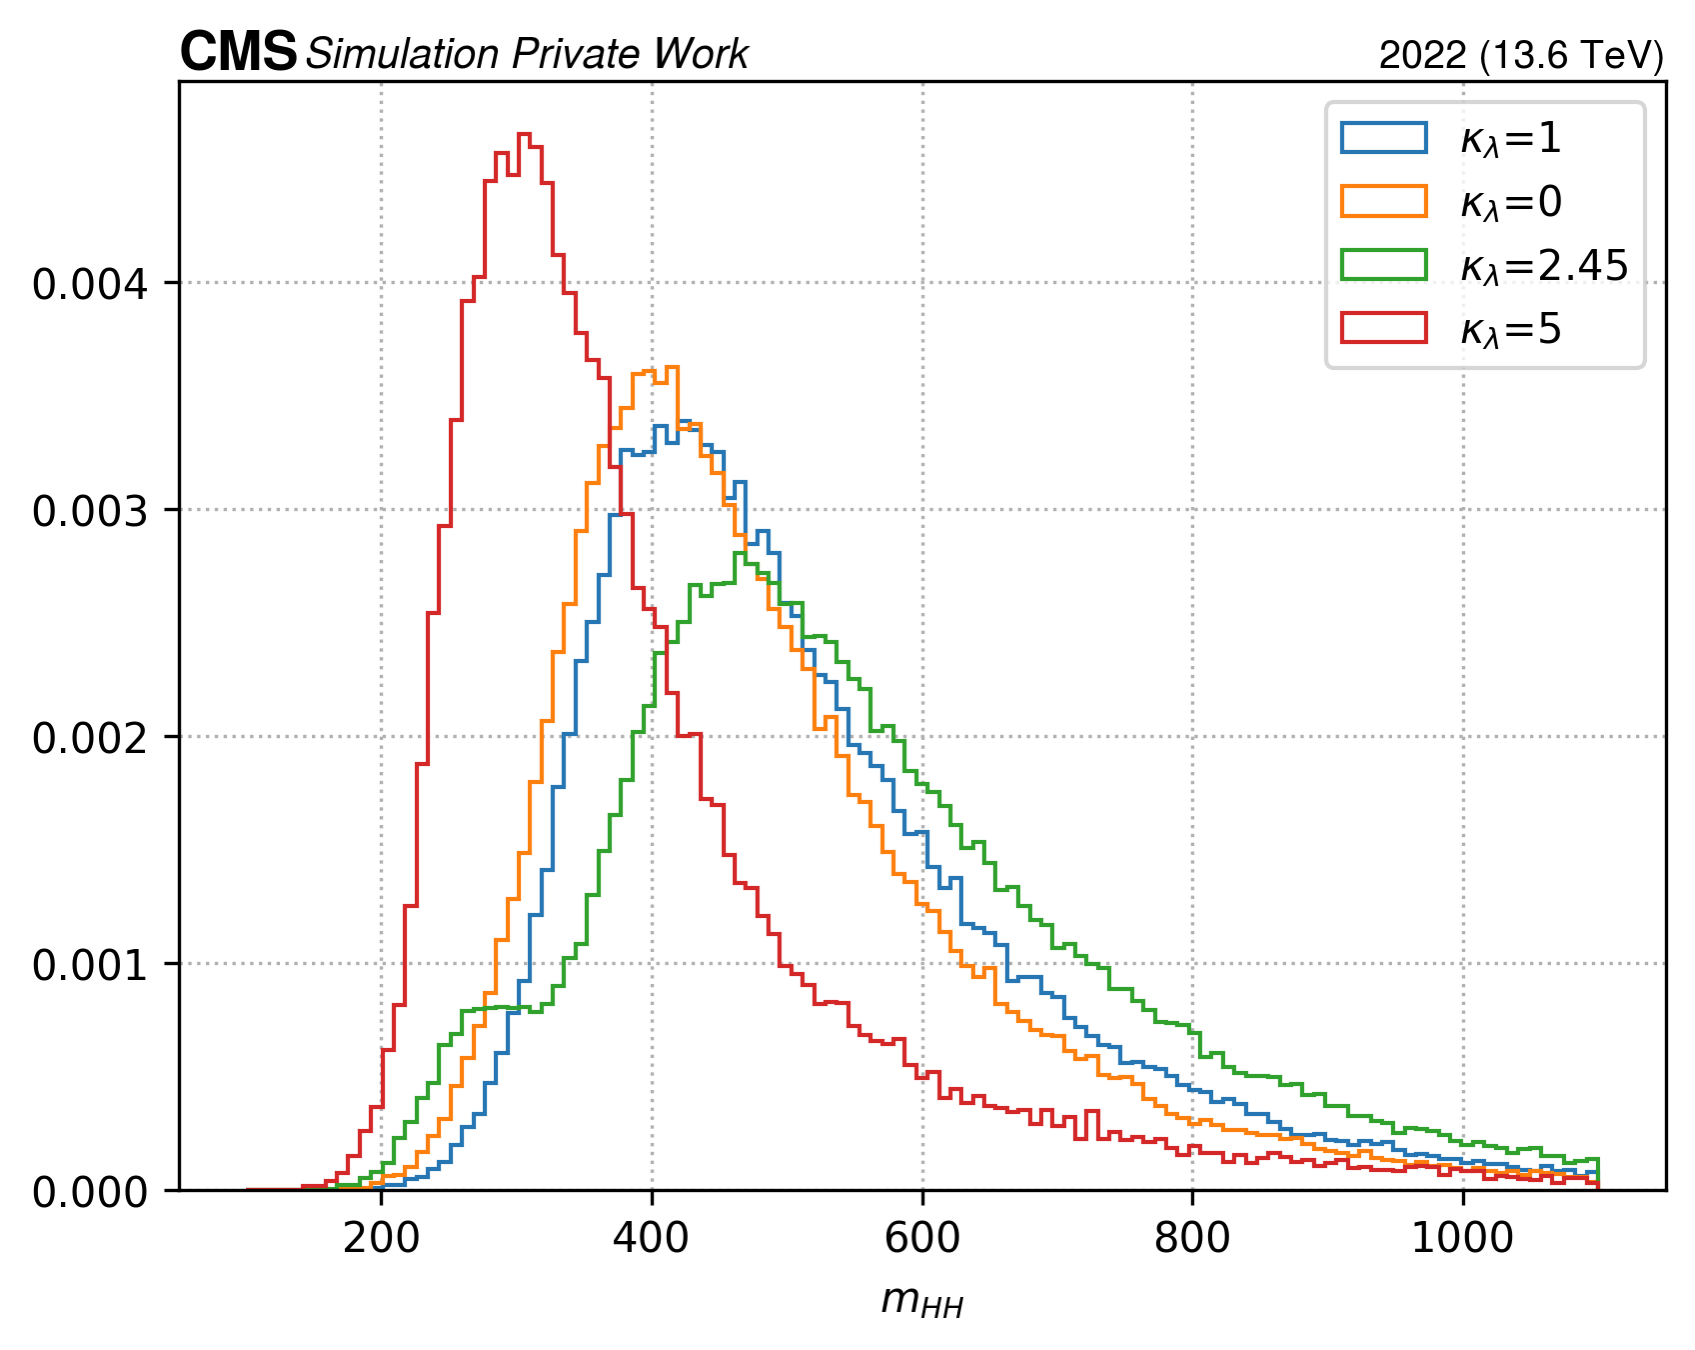
\includegraphics[width=0.5\linewidth]{Images/6.Improving/kappa lambda/mhh distribution for diff kl.png}
    \caption{$m_{HH}$ distribution for different values of \kl.}
    \label{fig: mhh dist}
\end{figure}


\vspace{0.2cm}

In this Section, we compare the difference of performance when training SPANet with \kl samples instead of SM samples. In addition, the difference in performance is compared when adding the explicit value of \kl per event as global input, i.e. adding the value of \kl per event. In order to do so, we compare the trainings presented in Table \ref{table:kl as input or not}. The naming "Tight cuts" refers to the Tight cuts presented in Section \ref{subsection:cutflows} that have been used in the previous sections. 

\begin{table}[h!]
\centering
    \begin{tabular}{|M{4cm}|M{7cm}|}
     \hline
     Training  & Configuration \\
     
     \hline
     
    SPANet - \kl - Tight selection &  5 jets as inputs:\footnotesize 
    \begin{itemize}[itemsep=0.001em]
        \item \pt
        \item $\eta$
        \item $\phi$
        \item b-tag
        \item Train file containing events with different \kl
        \item \kl not an explicit input to the network
    \end{itemize} \\
     
     \hline
     
    SPANet - \kl (\kl inputs)- Tight selection &  5 jets as inputs: \footnotesize 
    \begin{itemize}[itemsep=0.001em]
        \item \pt
        \item $\eta$
        \item $\phi$
        \item b-tag
        \item Train file containing events with different \kl
        \item \kl as global input
    \end{itemize} \\
     
     \hline
     
      SPANet - SM - Tight selection &  5 jets as inputs: \footnotesize 
    \begin{itemize}[itemsep=0.001em]
        \item \pt
        \item $\eta$
        \item $\phi$
        \item b-tag
        \item Train file containing only events with SM coupling 
    \end{itemize}\\    
     \hline
    \end{tabular}
    \caption{Training configurations used to test the difference when using SM samples or \kl samples. We also test the difference when adding \kl as an explicit input to the network.}
    \label{table:kl as input or not}
\end{table}


%Figures \ref{fig: kl kl input or no input} and \ref{fig: mhh kl input or no input} show the total pairing efficiency as a function of \kl and $m_{HH}$ respectively of the models presented in Table \ref{table:kl as input or not}.

Figure \ref{fig: kl kl input or no input} shows the total pairing efficiency as a function of \kl. It is observed that by training our model using a sample with different \kl, the pairing performance is improved with respect to the SPANet-SM training. However, we observe that using \kl as an explicit input to our network does not improve our performance. The same conclusion can be drawn from Figure \ref{fig: mhh kl input or no input}, where we show the total pairing efficiency as a function of $m_{HH}$. This is expected since \kl and $m_{HH}$ are correlated. Especially, in the low $m_{HH}$ mass region, a large improvement is observed compared to the trainings using only SM samples. This improvement in the pairing efficiency with respect to the training using SM samples is expected as well, since by adding events with different \kl as shown in Figure \ref{fig: mhh dist}, new events are added in the low $m_{HH}$ spectrum for the training. Finally, in both Figures \ref{fig: kl kl input or no input} and \ref{fig: mhh kl input or no input}, it is observed that the SPANet pairing efficiency outperforms the Run 2 approach on the $D_{HH}$-method.

\begin{figure}[hbt]
    \centering
    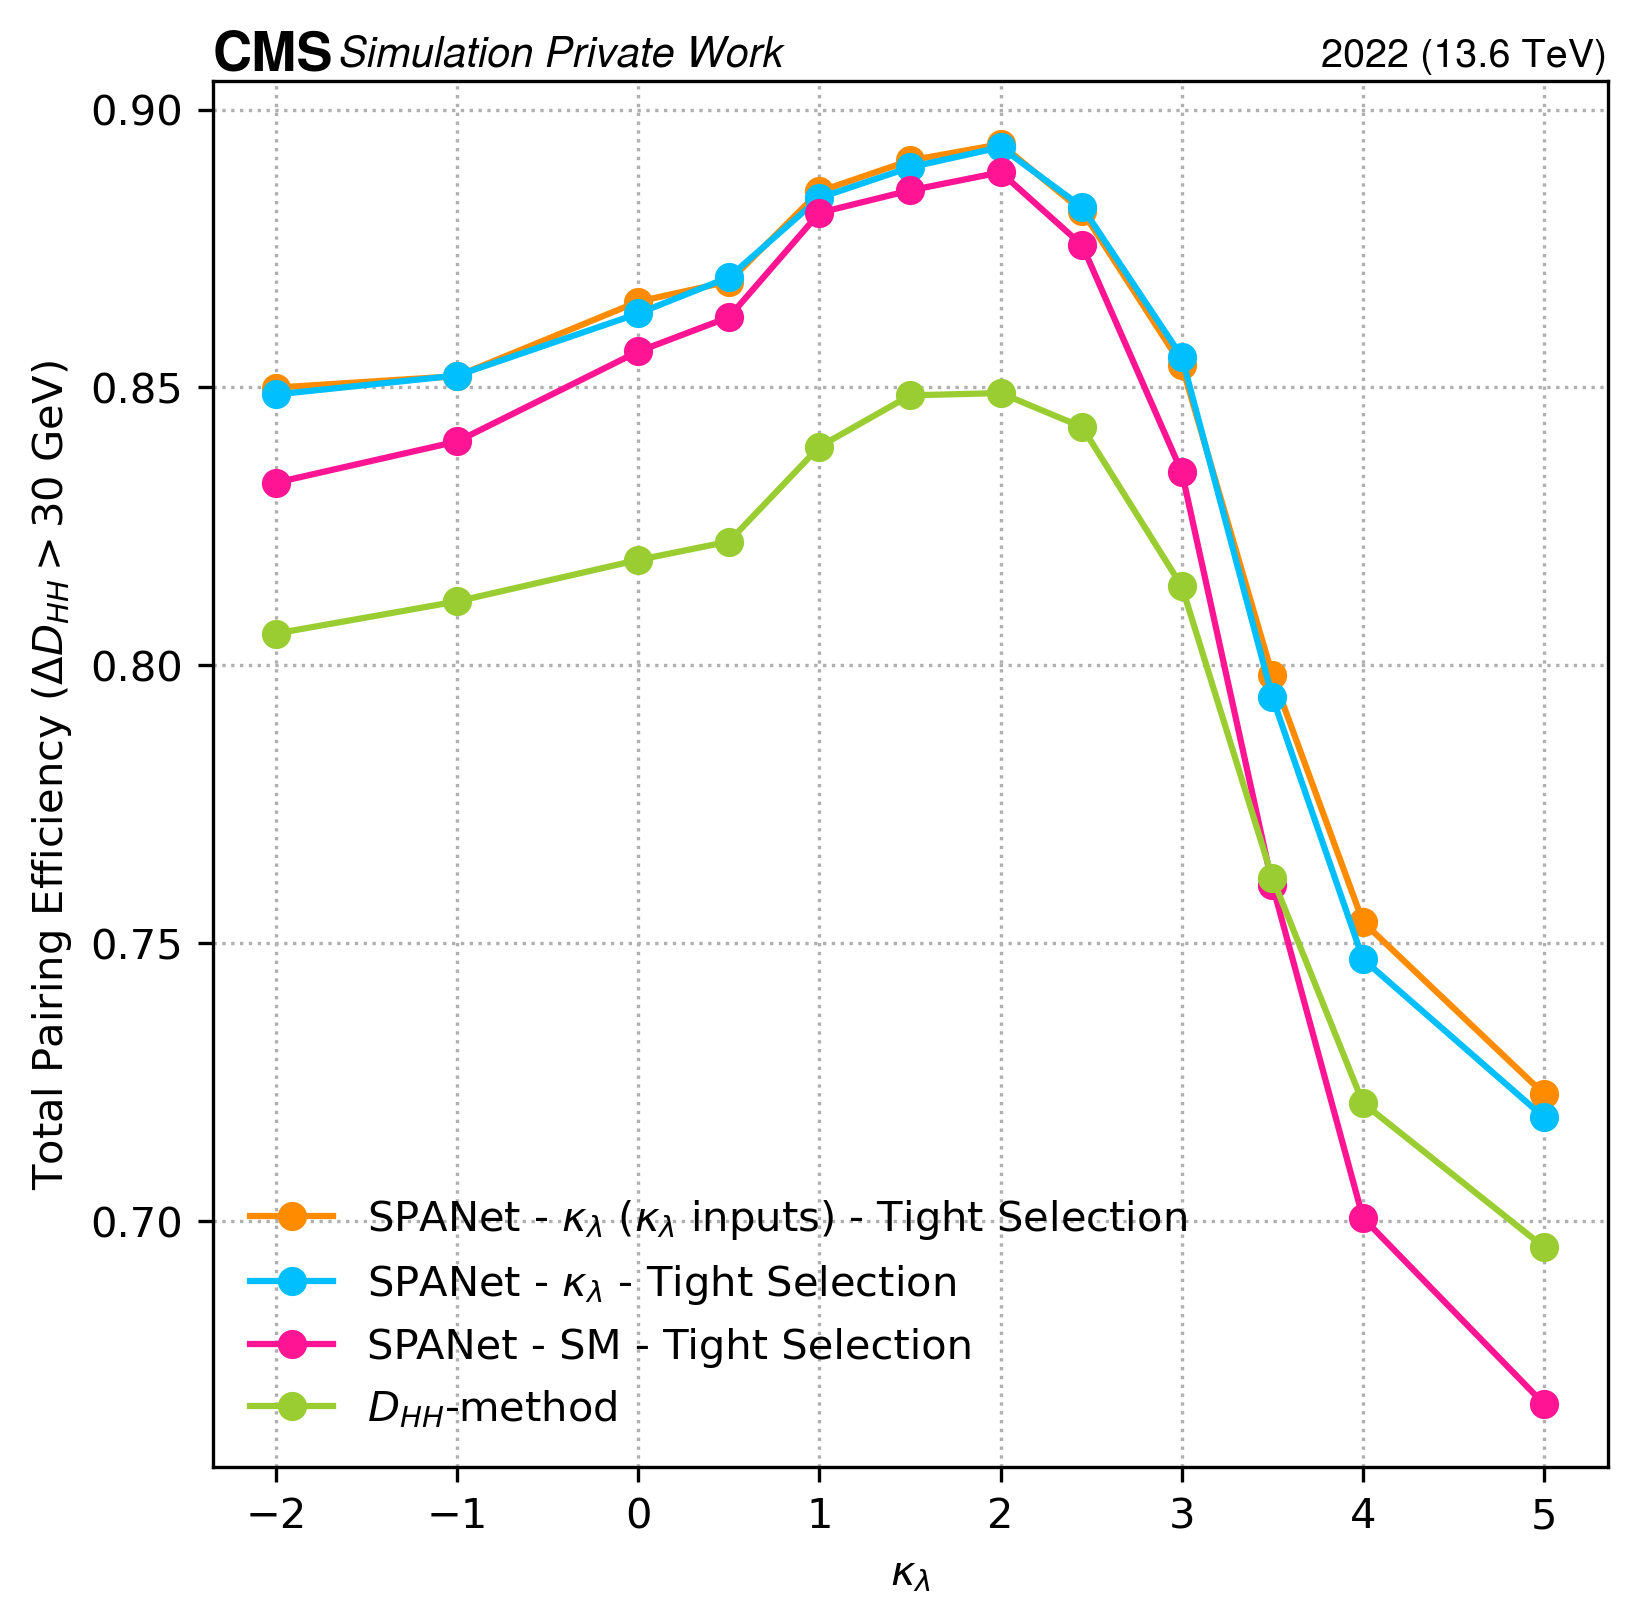
\includegraphics[width=0.6\linewidth]{Images/6.Improving/kappa lambda/kl inout vs no input.png}
    \caption{Total pairing efficiency as a function of \kl for the different training configuration presented in Table \ref{table:kl as input or not}.}
    \label{fig: kl kl input or no input}
\end{figure}

\begin{figure}[hbt]
    \centering
    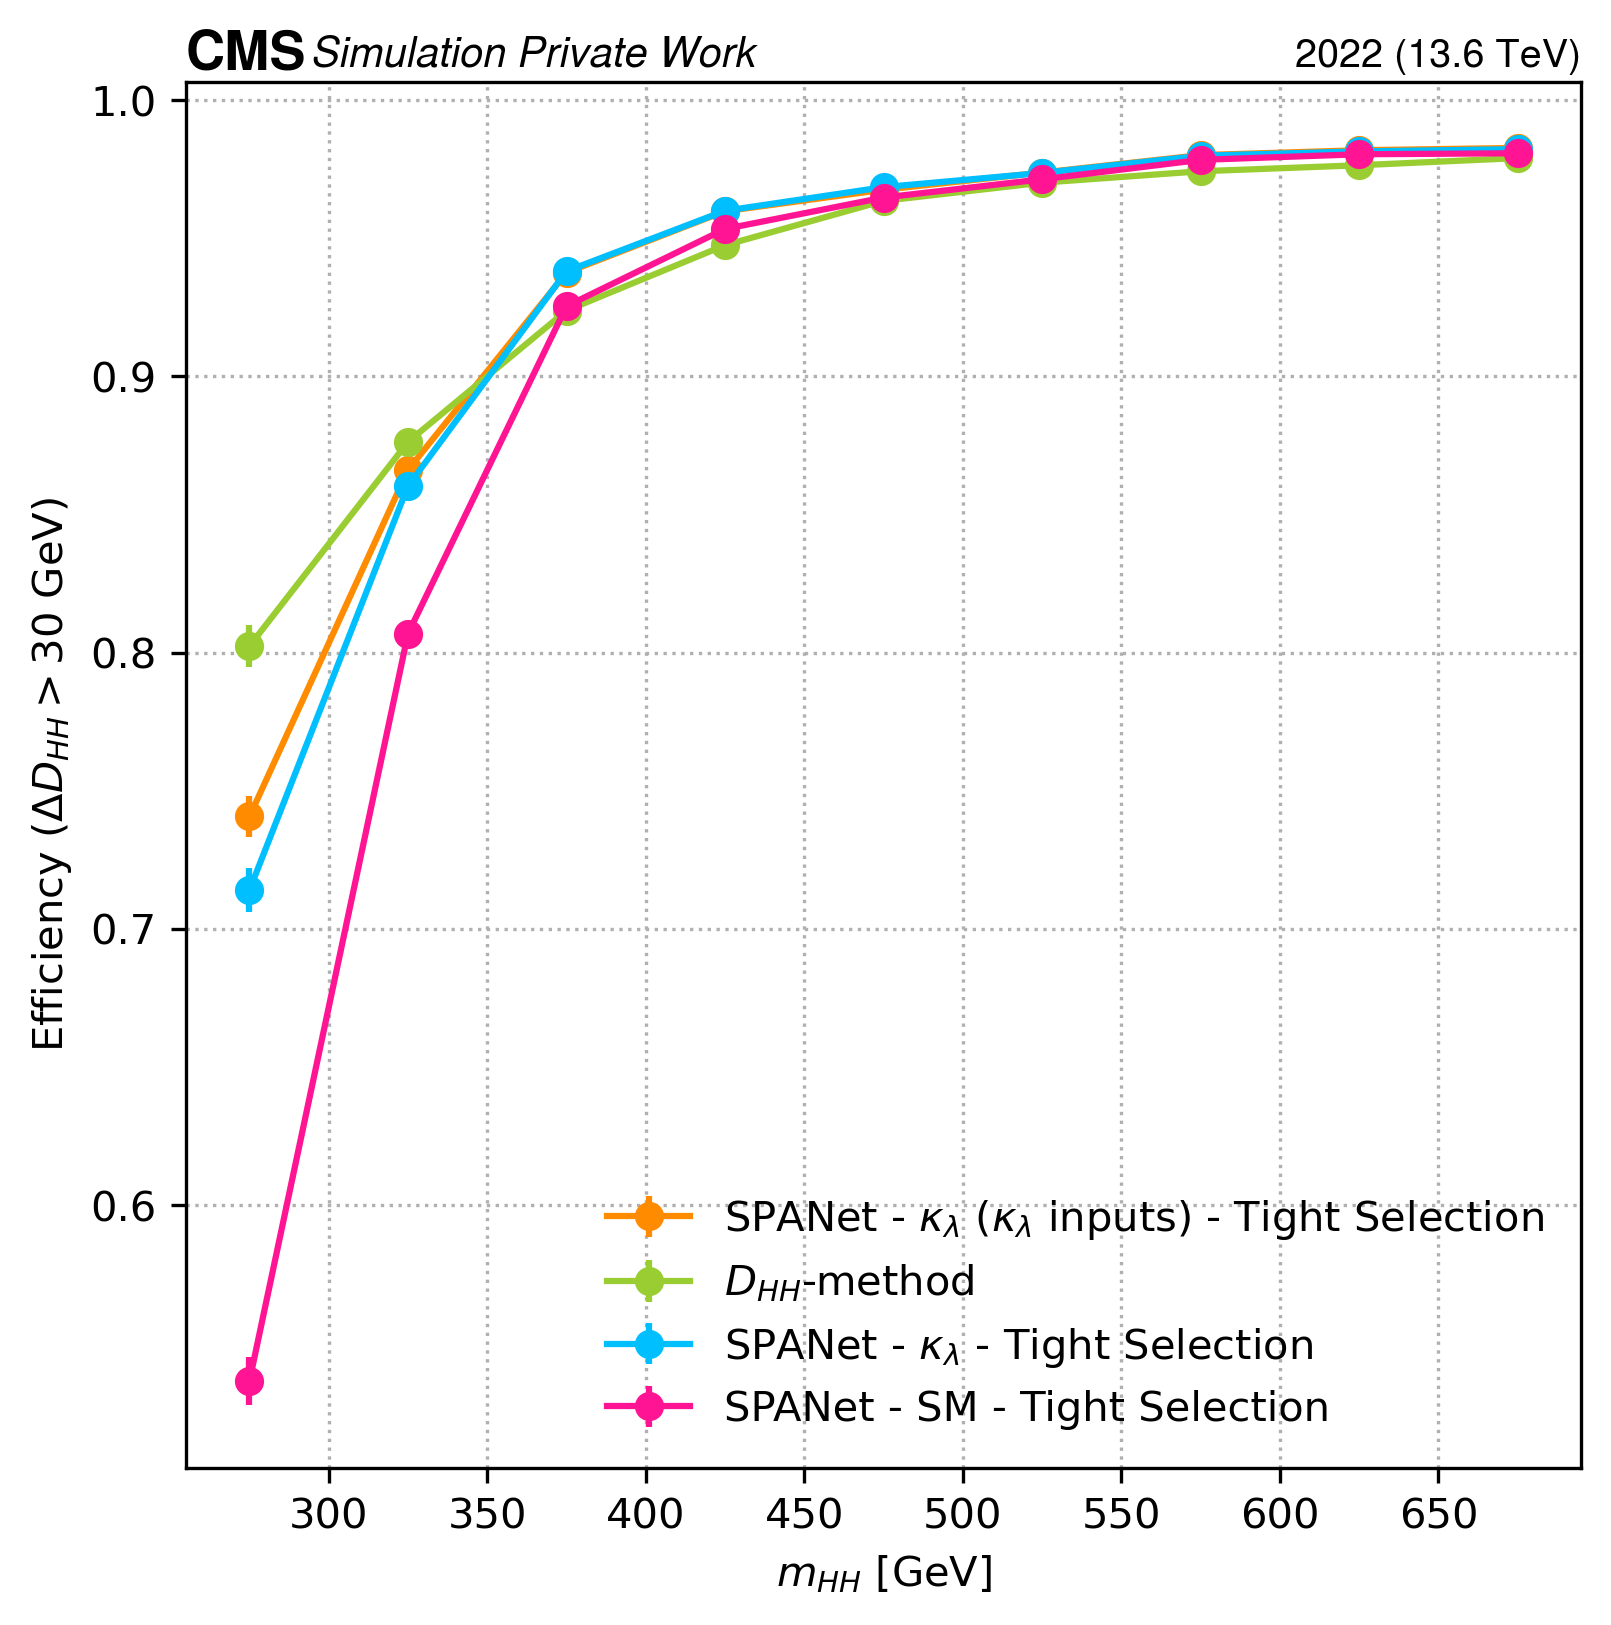
\includegraphics[width=0.6\linewidth]{Images/6.Improving/kappa lambda/eff diff kl vs kl input.png}
    \caption{Total pairing efficiency as a function in $m_{HH}$ for the different training configuration presented in Table \ref{table:kl as input or not}.}
    \label{fig: mhh kl input or no input}
\end{figure}

Figures \ref{fig: kl kl input or no input} and \ref{fig: mhh kl input or no input}  show that adding \kl as an explicit input does not improve the SPANet efficiency. Therefore, the model in which \kl is not explicitly added as input is chosen since, when the model is evaluated on either data or QCD,  it is ambiguous which value of  \kl should be given as input to the network.  Hence, the SPANet - \kl - Tight selection model is chosen.

Table \ref{table: improvement} shows the values of the pairing efficiency as well as the total pairing efficiency for \kl $\in \{ 0, 1, 5 \} $ with the best SPANet training model. It is observed that by using the training SPANet - \kl - Tight selection, we have {4-8\%} absolute improvement with respect to the $D_{HH}$-method, as well as a {5-14\%} relative improvement. 

\begin{table}[h!]
\centering
\begin{tabular}{|M{2.5cm}||M{1.75cm}|M{1.75cm}||M{1.75cm}|M{1.75cm}||M{1.75cm}|M{1.75cm}|}
 \hline
 Training  & Pairing efficiency (\kl=1) &  Total pairing efficiency (\kl=1) & Pairing efficiency (\kl=0) &  Total pairing efficiency (\kl=0) & Pairing efficiency (\kl=5) &  Total pairing efficiency (\kl=5) \\
 \hline
  $D_{HH}$-method &  0.944 &  0.836 & 0.921 & 0.808 & 0.739 & 0.603\\
 \hline
 SPANet - \kl - Tight selection & 0.952  &  0.880 & 0.932 & 0.853 & 0.792 & 0.685 \\
 \hline
\end{tabular}
\caption{Comparison of the pairing efficiency and the total pairing efficiency between the $D_{HH}$-method and the training SPANet - \kl - Tight selection.}
\label{table: improvement}
\end{table}

\subsection{Impact of different kinematic selections in the analysis}

In the previous sections, Tight cuts (defined in Section \ref{subsection:cutflows}) were applied to the samples used for training and evaluation. Nevertheless, we checked the comparison between models trained on different sets of kinematic selections when evaluating the model on samples where Loose cuts are applied (defined in Section \ref{subsection:cutflows}). The configuration of training used for the comparison is reported in Table \ref{table:kl loose vs tight}.


\begin{table}[h!]
\centering
\begin{tabular}{|M{2.5cm}|M{6cm}|}
 \hline
 Training  & Configuration  \\
 \hline
  SPANet - \kl - Tight selection &  5 jets as inputs:\footnotesize \begin{itemize}[itemsep=0.001em]
    \item \pt
    \item $\eta$
    \item $\phi$
    \item b-tag
    \item Tight cuts
    \item Train file containing events with different \kl but these are not given as explicit inputs to the network
 \end{itemize}  \\
 \hline
 SPANet - \kl - Loose selection &  5 jets as inputs: \footnotesize \begin{itemize}[itemsep=0.001em]
    \item \pt
    \item $\eta$
    \item $\phi$
    \item b-tag
    \item Loose cuts
    \item Train file containing events with different \kl but these are not given as explicit inputs to the network
 \end{itemize}  \\
 \hline
\end{tabular}
\caption{Configuration of trainings using a sample containing events with different \kl.}
\label{table:kl loose vs tight}
\end{table}

Figure \ref{fig: loose vd tight} shows the total pairing efficiency as a function of \kl for the trainings presented in Table \ref{table:kl loose vs tight} both evaluated on the test file in which the Loose cuts are applied. We also compare them to the $D_{HH}$-method used in Run 2. From this figure, we can see that the performance is the same for the two trainings within the variability and that they both outperform the $D_{HH}$-method. Nevertheless, the test of the background mass sculpting presented in Figures \ref{fig: leading H mass dist} and \ref{fig: subleading H mass dist} shows that there is a significant difference between training on Loose or Tight cuts. We conclude that training on Loose cuts sculpts significantly more the mass of both the leading and the subleading Higgs. Since the significant background sculpting associated with the Loose selection is an unwanted feature of our model, the best SPANet training configuration makes use of Tight cuts.

\begin{figure}[hbt]
    \centering
    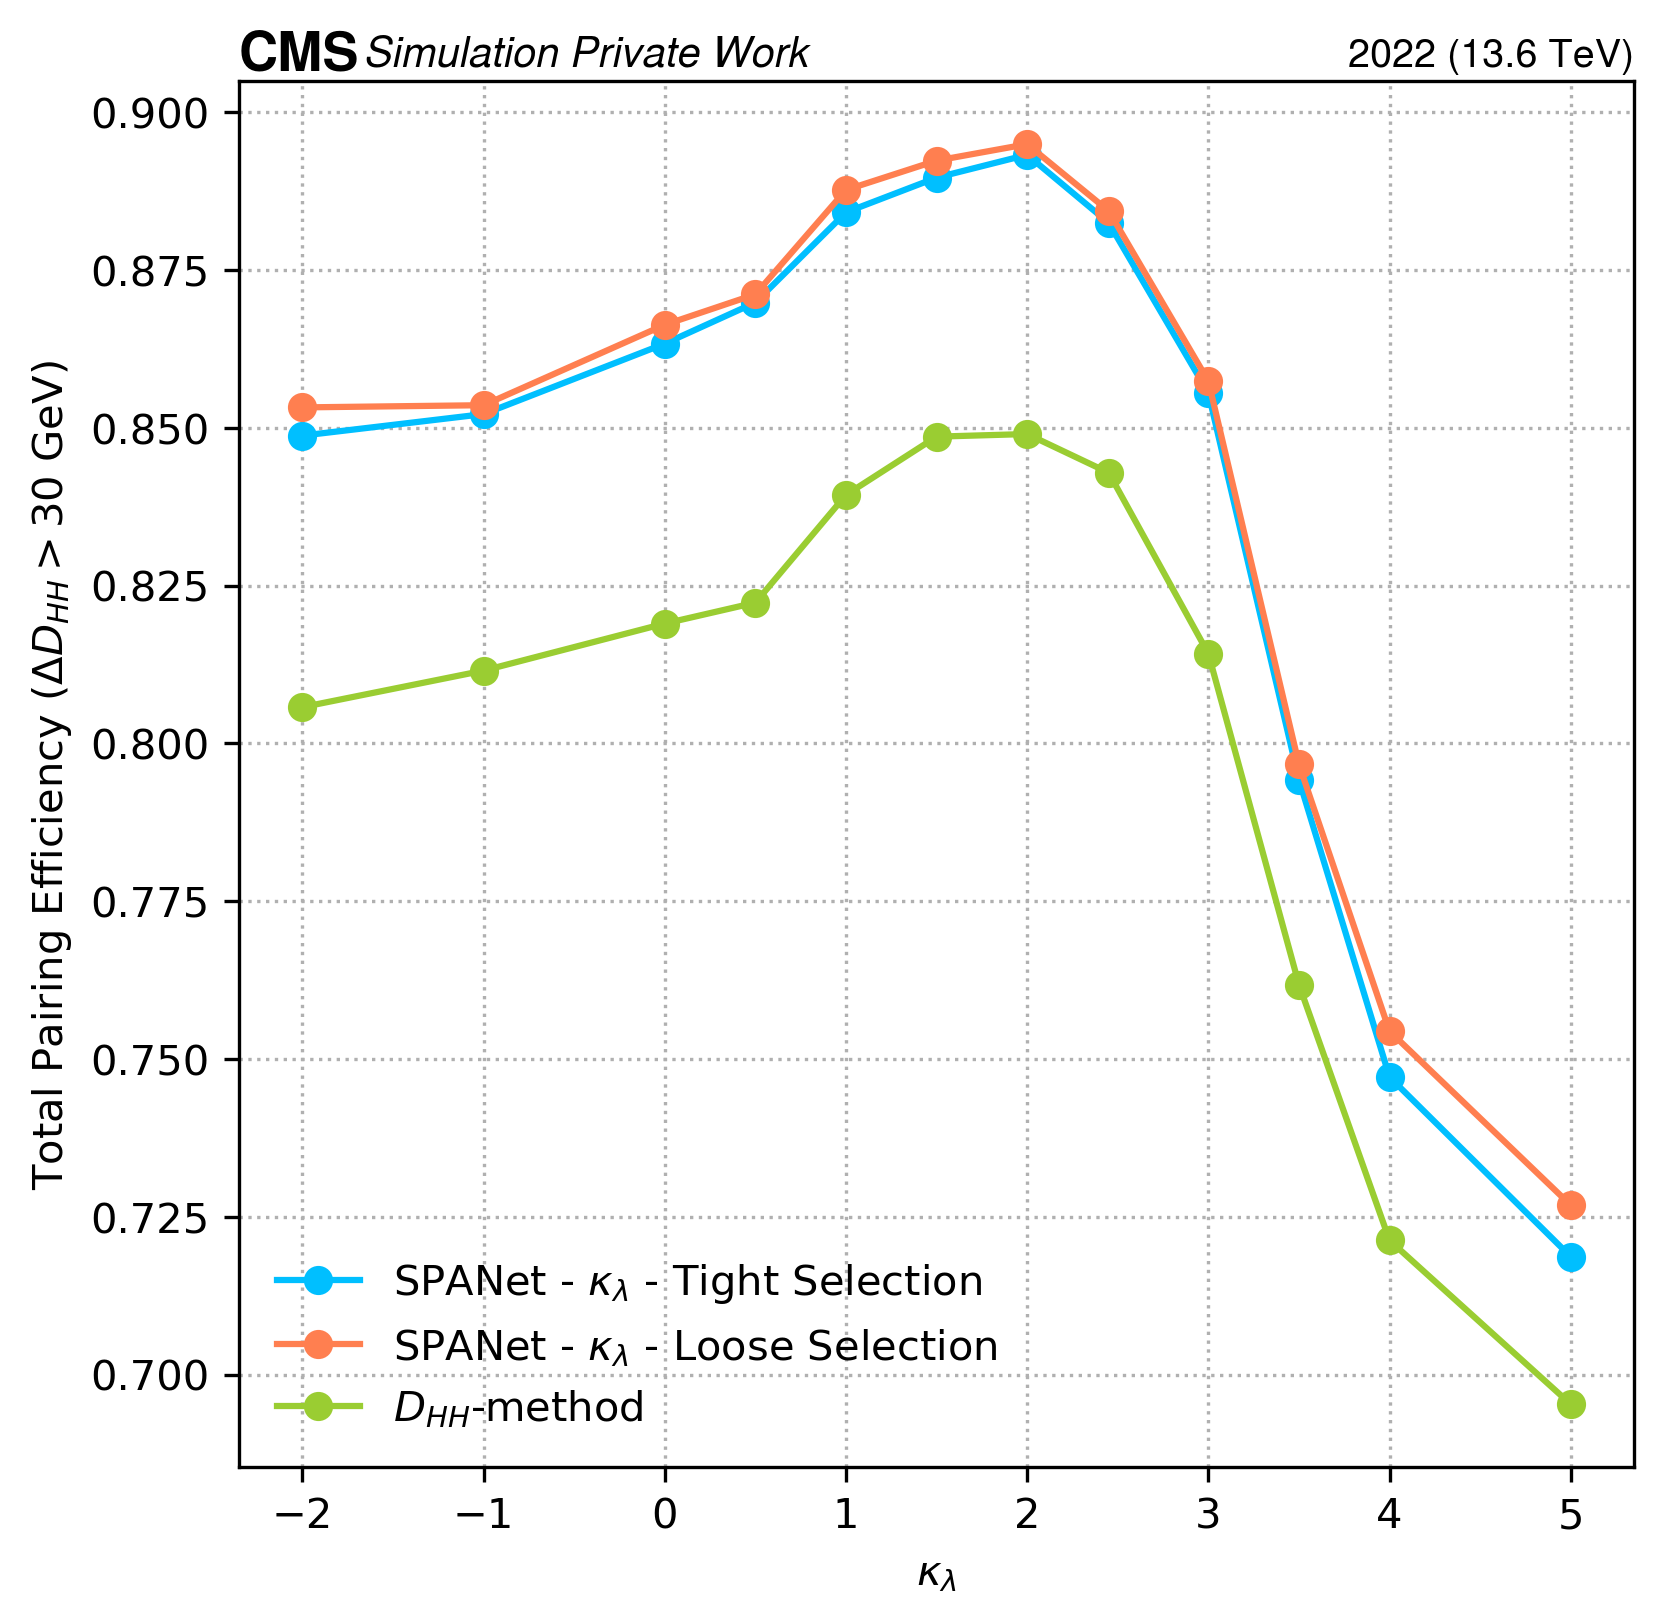
\includegraphics[width=0.6\linewidth]{Images/6.Improving/kappa lambda/loose vs tight.png}
    \caption{Comparison of trainings using Loose or Tight cuts presented in Table \ref{table:kl loose vs tight}). These trainings are compared to the $D_{HH}$-method used in Run 2.}
    \label{fig: loose vd tight}
\end{figure}

\begin{figure}[hbt]
    \centering
    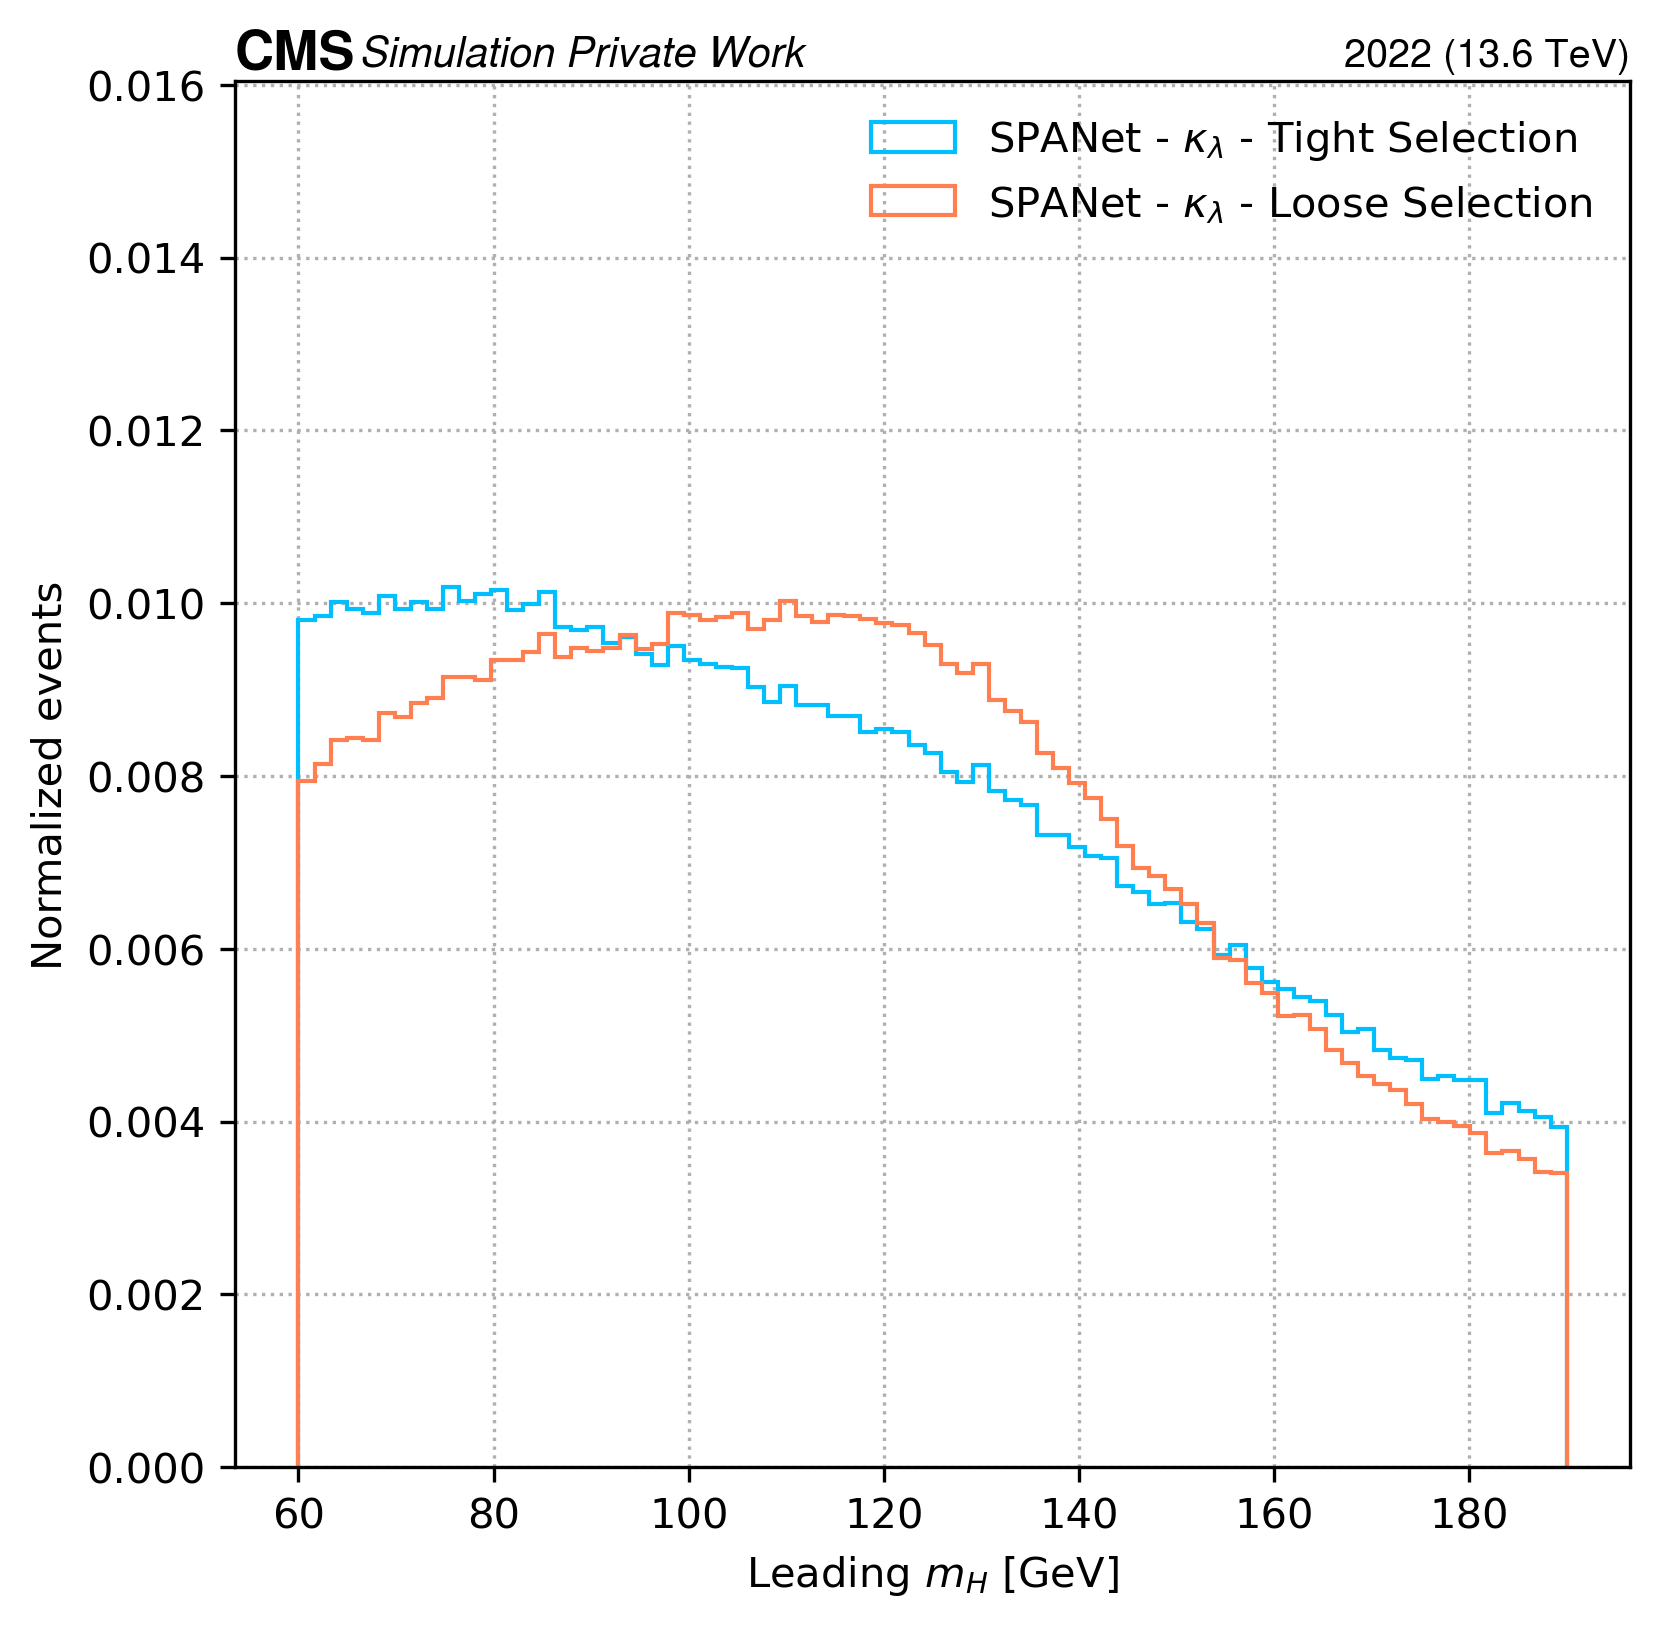
\includegraphics[width=0.6\linewidth]{Images/6.Improving/kappa lambda/leading h mass sculp.png}
    \caption{Distribution of the leading Higgs mass after evaluating the models presented in Table \ref{table:kl loose vs tight} on 2b data.}
    \label{fig: leading H mass dist}
\end{figure}

\begin{figure}[hbt]
    \centering
    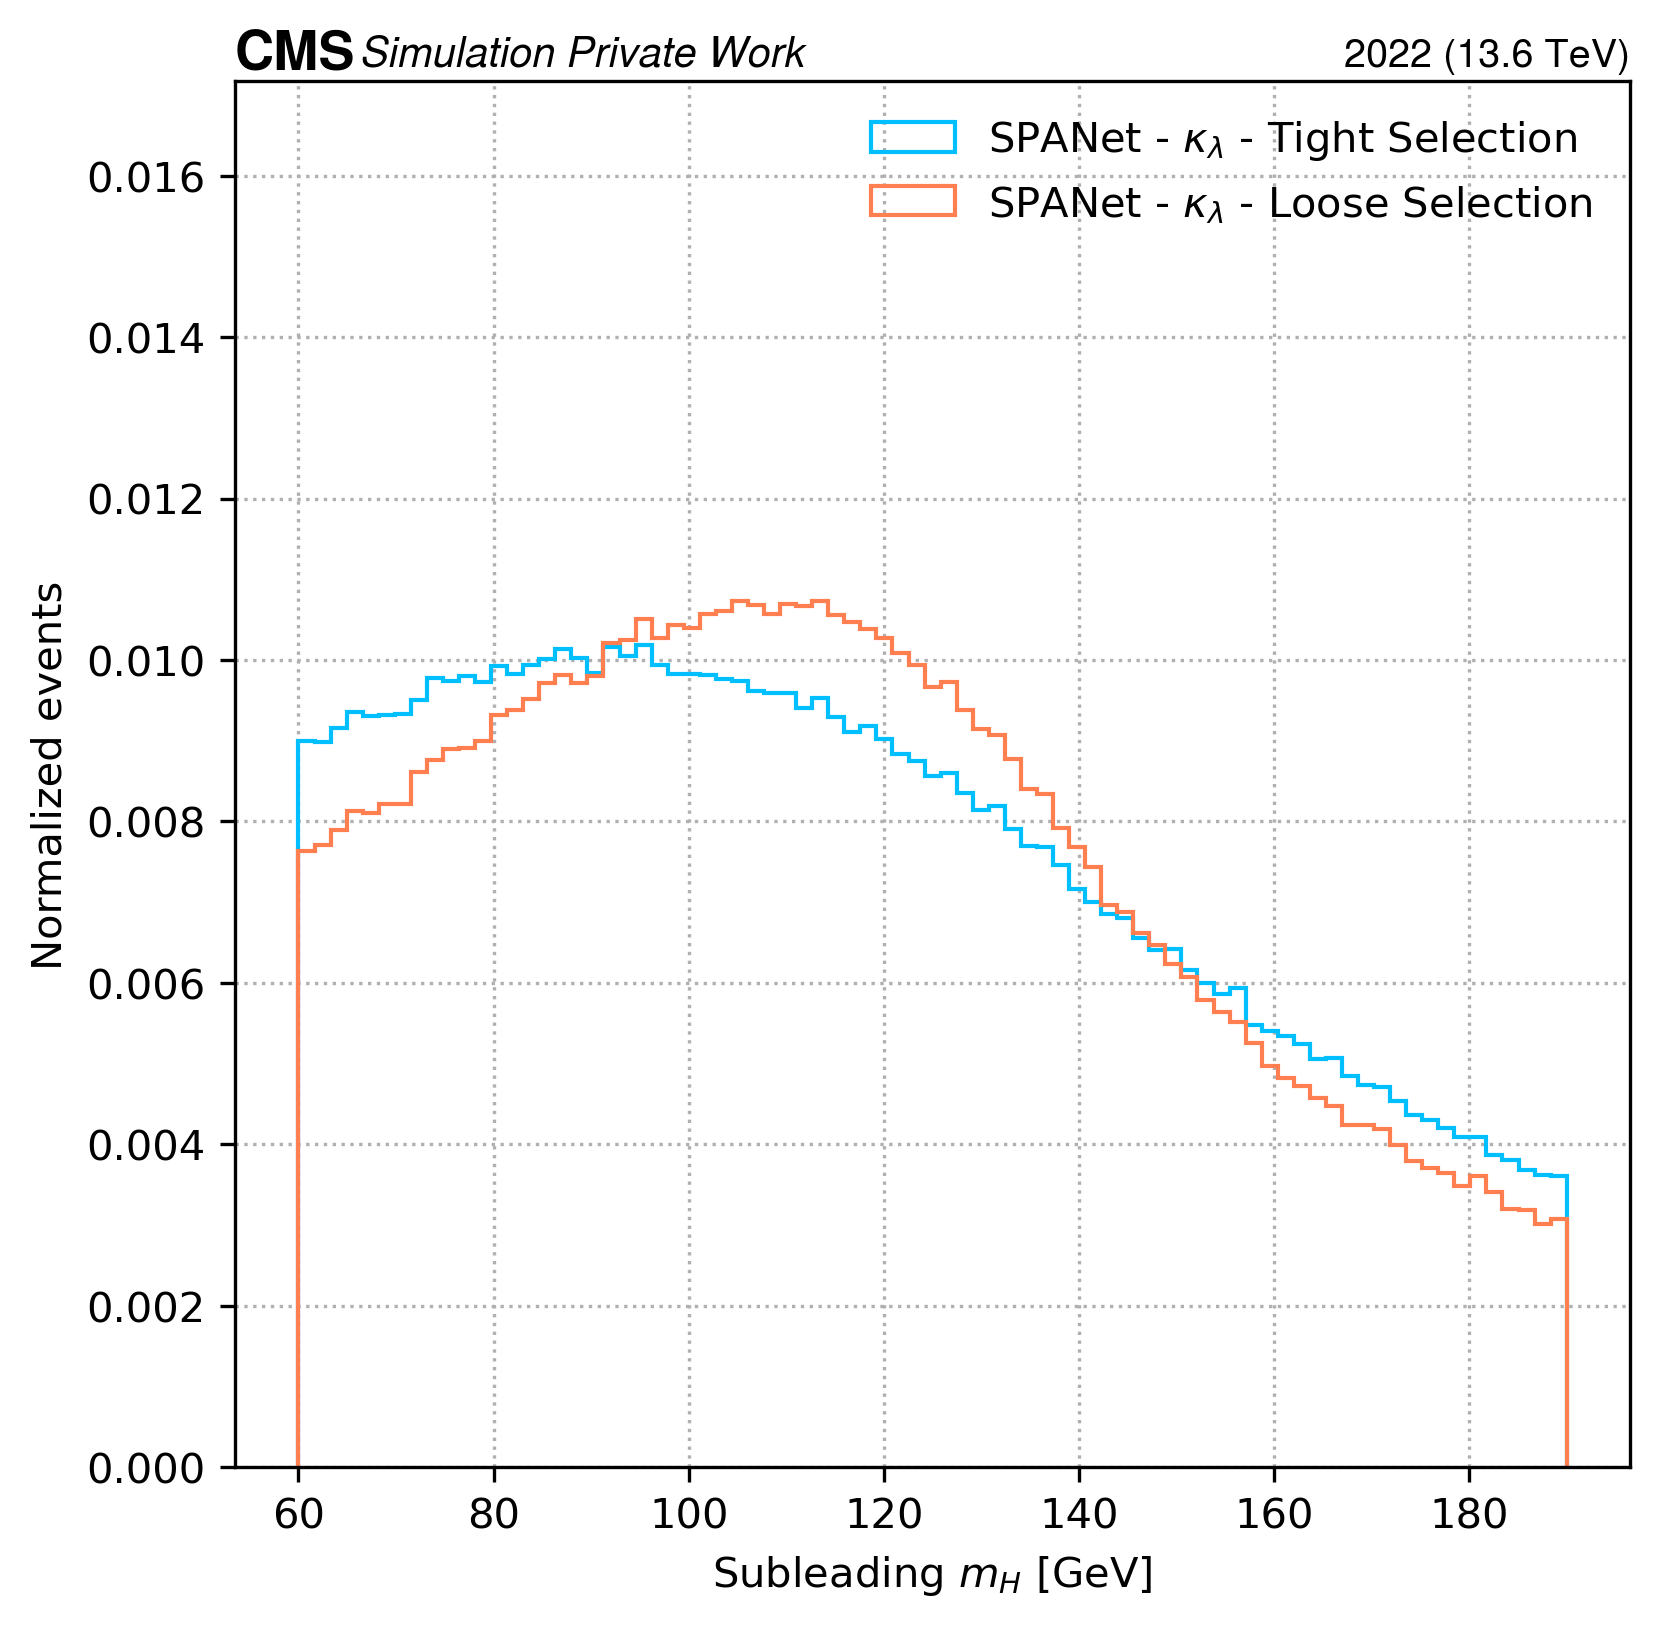
\includegraphics[width=0.6\linewidth]{Images/6.Improving/kappa lambda/sub leading H mass sculpt.png}
    \caption{Distribution of the subleading Higgs mass after evaluating the models presented in Table \ref{table:kl loose vs tight} on 2b data.}
    \label{fig: subleading H mass dist}
\end{figure}

\newpage

\subsection{The final configuration} \label{subsection: Optimal config}
After comparing several configurations, we conclude that the best performance for jet pairing is given by the SPANet - \kl - Tight selection model that uses:
\begin{itemize}
    \item \pt regressed, $\eta$, $\phi$ and b-tag of the 5 jets considered for the pairing as sequential inputs
    \item No explicit \kl input as a global variable
    \item Stable model hyperparameters (shown in Table \ref{table: stable model})
\end{itemize}
Figure \ref{fig: 2D mass dist kl} shows the 2D mass sculpting of the background. We do not observe any excess of events (background sculpting) in the SR.

\begin{figure}
    \centering
    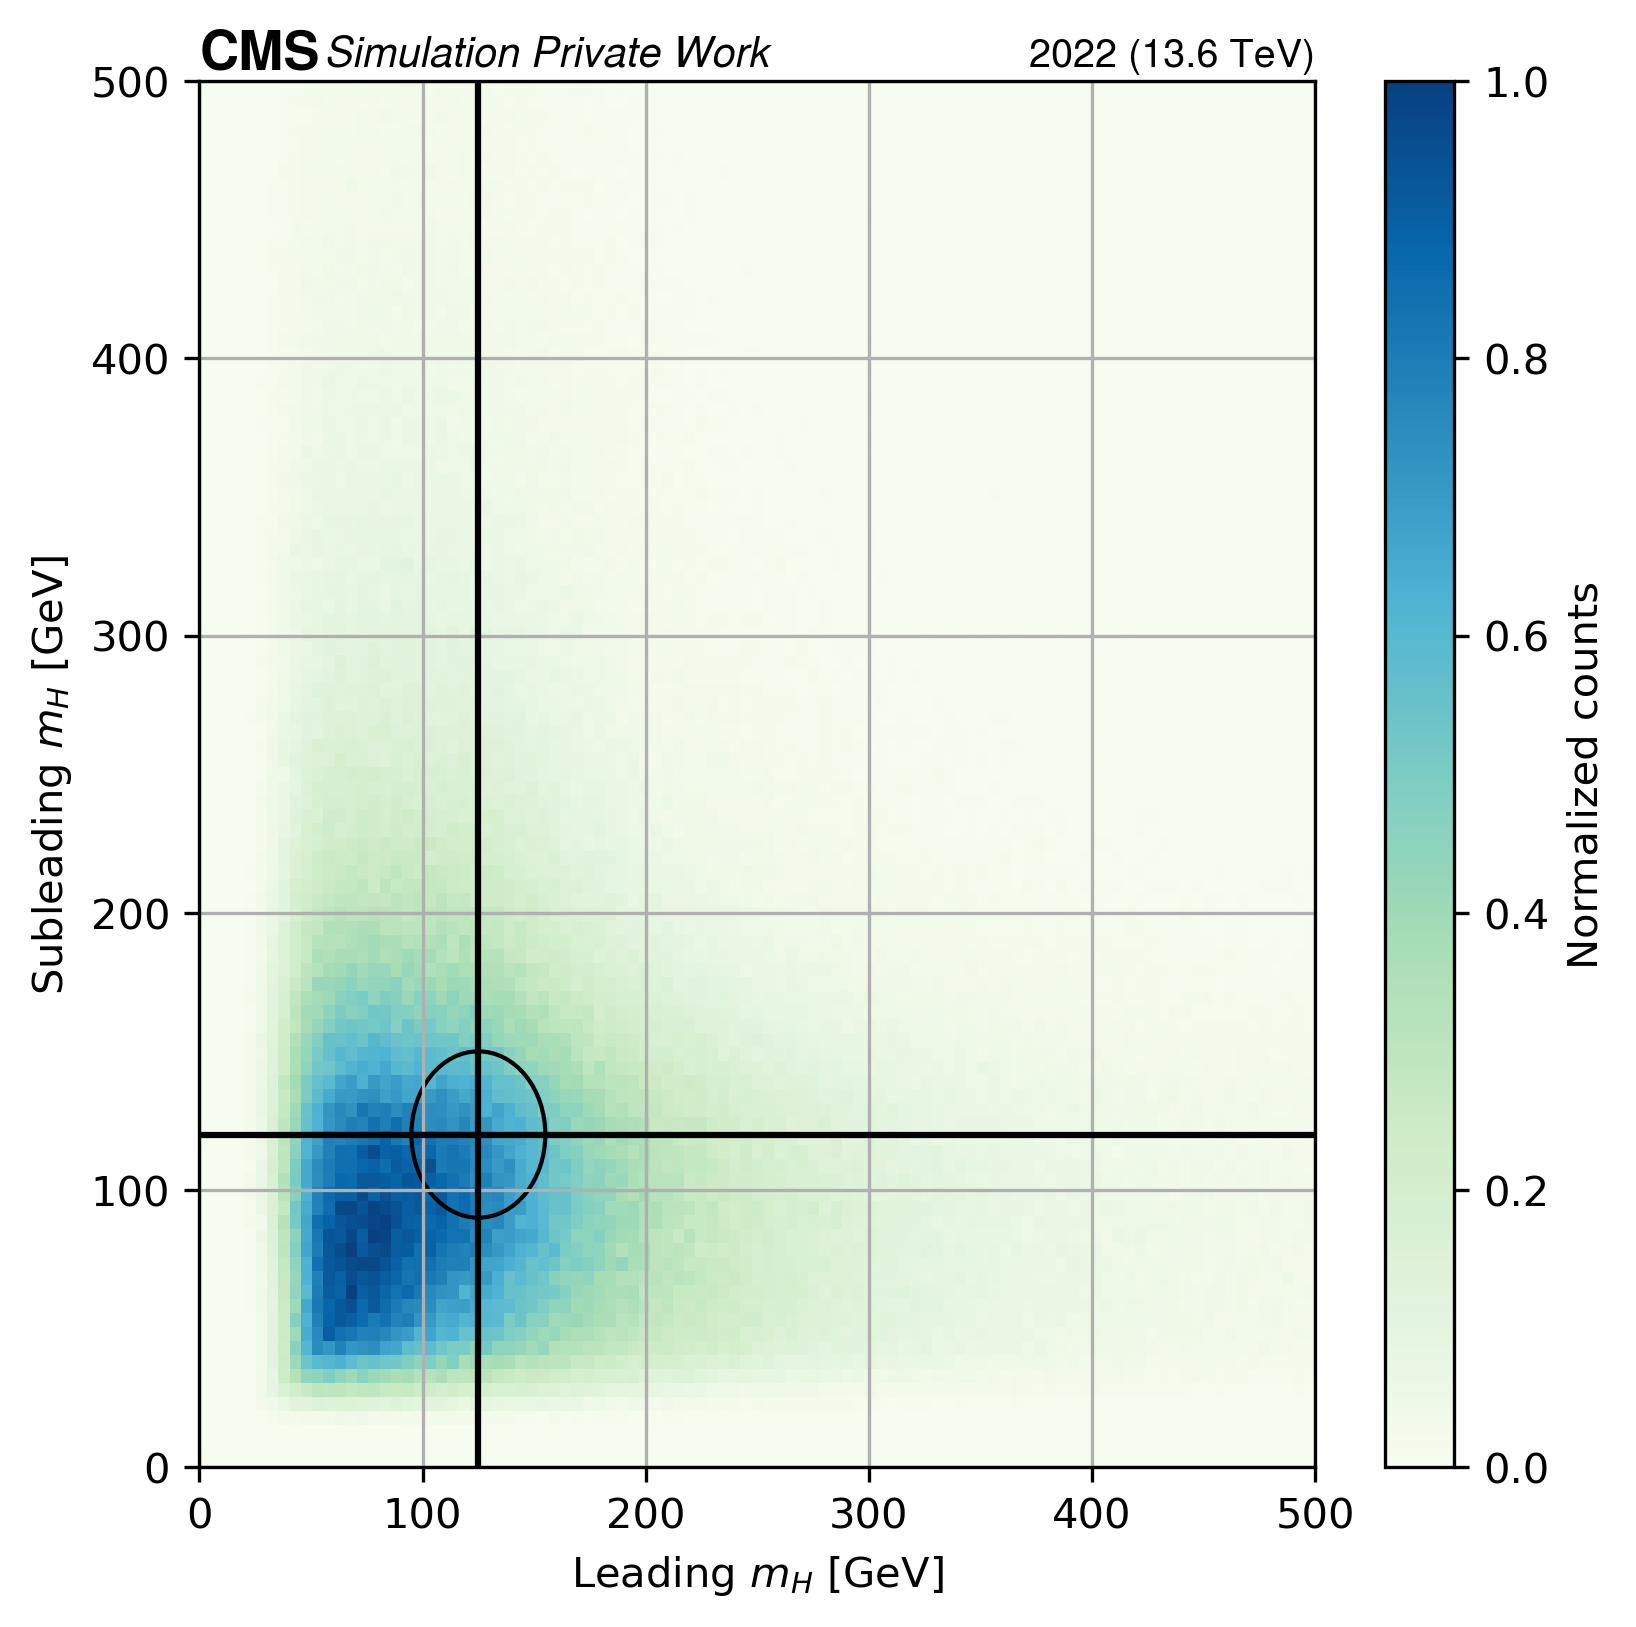
\includegraphics[width=0.6\linewidth]{Images/6.Improving/kappa lambda/mass dist best model.png}
    \caption{Higgs mass distribution of the leading Higgs and the subleading Higgs after the evaluation of  SPANet - \kl - Tight selection model on 2b data. The vertical black line corresponds to the mass of the leading Higgs and the horizontal of the subleading Higgs. The black circle defines the SR area defined in Section \ref{section: HH4b}.}
    \label{fig: 2D mass dist kl}
\end{figure}

% jets as inputs, pt regressed, lite and stable model, tight cuts, no kl as inout explicitely